\documentclass[11pt,a4paper,leqno]{report}

\usepackage{kandi}

% useful definitions

\newcommand{\Author}{Aaro Salosensaari}
\newcommand{\Title}{Mallinnettu jäähdytys ja ympyräkiekkojen etsiminen kuvasta}

\usepackage{hyperref}          % linkit ja pdf-toc
\hypersetup{
    pdfencoding=auto,
    colorlinks=false,
    hidelinks,
    pdftitle={\Title},
    pdfauthor={\Author}
}

\usepackage{csquotes}
\usepackage[hyperref=true, style=alphabetic]{biblatex}
\bibliography{bibkandi}

% confiugre table of cont
\setcounter{tocdepth}{1}

\begin{document}

    \title{\Title}

    \author{\Author\\
        \small{ \texttt{\href{mailto:aaro.salosensaari@helsinki.fi}{aaro.salosensaari@helsinki.fi}}}
    }

    \date{\today}


    %\maketitle
    % kandidaatintutkielma titlepage
\begin{titlepage}
    \begin{center}
        {\large Kandidaatintutkielma}

        \vspace{\baselineskip}

        {\Large \bfseries \Title}

        \vspace{2\baselineskip}

        {\large \Author}\\
        %{\small{ \texttt{\href{mailto:aaro.salosensaari@helsinki.fi}{aaro.salosensaari@helsinki.fi}}}}


        \vfill

        {\large
            Soveltava matematiikka\\
            Matematiikan ja tilastotieteen laitos\\
            Helsingin Yliopisto
        }

        \vspace{2\baselineskip}

        {\large Helsinki, \today}
    \end{center}
\end{titlepage}


    % sisallys
    {\small
        \tableofcontents
    }

    \chapter{Johdanto}
\label{cha:johdanto}

% erillinen abstrakti palautuspdf:ään.

Tämä soveltavan matematiikan kandidaatintutkielma käsittelee matemaattisen optimoinnin menetelmää nimeltä mallinnettu jäähdytys ja sen soveltamista digitaalisen kuvankäsittelyn ja keinonäön ongelmaan: ympyräkiekkojen etsimiseen sumeasta ja kohinaisesta kuvasta.
Kuvaongelman muotoilun yhteydessä esitellään myös digitaalisen kuvankäsittelyn perusteita.

Mallinnettu jäähdytys (engl. \emph{simulated annealing}, suomeksi myös \emph{jäähdytysmenetelmä} tai \emph{simuloitu jäähdytys} \cite[suomennokset ks.][]{haataja93}, myöhemmin lyhyesti SA tai SA-algoritmi) on tunnettu probabilistinen optimointialgoritmi (terminologiasta riippuen myös optimointiheurestiikka tai metaheurestiikka) globaalin, tavallisesti diskreetin tai kombinatorisen optimointitehtävän ratkaisemiseksi.
Jäähdytysalgoritmin esittelivät \citeauthor*{kirkpatrick83} 1983 artikkelissa \cite{kirkpatrick83} Metropolis-Hastings-algoritmin sovelluksena erilaisiin kombinatorisiin optimointiongelmiin, kuten kuuluisaan kauppamatkustajan ongelmaan.
Metropolis-algoritmi vuorostaan on klassinen Markovin ketjujen Monte Carlo -menetelmä, jonka juuret ovat jäähtyvän fysikaalisen systeemin simuloinnissa.
Mallinnettu jäähdytys on yksinkertainen ja monikäyttöinen heurestiikka,
jonka hyödyllinen ominaisuus on sen kyky kiivetä ylös energiafunktion paikallisten minimien ''energiamaisemaan'' aiheuttamista kuopista~\cite{salamonetal}.

SA:lla on myös mielenkiintoisia yhtymäkohtia kvanttilaskentaan.
Metodin lähisukulainen nk. kvanttijäähdytys (\emph{quantum annealing}) perustuu siihen että monia kombinatorisia optimointiongelmia,
kuten verkon kahtiajako-ongelma, voidaan esittää spin-lasien Ising-mallin matalaenergisimpien tilojen etsintänä samaan tapaan kuin SA mallintaa termodynaamisen systeemin matalaenergisten tilojen löytämistä \cites[luku 4.5]{laarhoven}[]{johnson11dwave}.
Kvanttijäähdytysalgoritmi on väitetysti tehokas optimointimenetelmä, jos käytettävissä on sopivasti konstruoitu Ising-spin-systeemiä mallintava kvanttitietokone,
tai ainakin D-Wave Systems, Inc., esittää kykenevänsä huomattavaan laskentanopeuden parannukseen tällaisella laitteella \cite{johnson11dwave, denchev2015},
mutta nopeushypyn merkittävyydestä ei ole vielä selvyyttä \cite{troyer2015}.

Tutkielmassa mallinnettuun jäähdytykseen tutustutaan soveltamalla sitä yksinkertaiseen kuvankäsittelyongelmaan,
jossa tehtävänä on tunnistaa tunnettu määrä $k$ tummia ympyräkiekkoja sumentuneesta ja kohinaisesta vaaleataustaisesta kuvasta.
Tutkittavaa kuvaongelmaa lähestytään optimointiongelmana:
Tutkittavista kuvista muodostetaan malli, jossa kuvan ympyräkiekot parametrisoidaan niiden sijantikoordinaattien ja säteiden avulla
ja kiekkojen sumennosta mallinnetaan kuvamatriisin konvoluutio-operaatiolla.
Minimoitavaksi \emph{kohde- eli energiafunktioksi} valitaan sopiva parametrisoitujen kiekkojen etäisyyttä kuvadatasta mittaava funktio $E$.
Energiafunktiota minimoimalla voidaan etsiä parametrit, jotka määräävät kuvadataan parhaiten sopivat kiekot.

Tutkielman pääpainopiste on mallinnetussa jäähdytyksessä ja sen käyttäytymisen tutkimisessa kuvatussa esimerkkiongelmassa.
Esitetty ympyräongelma ja valittu kuvamalli on reaalimaailman sovelluksia ajatellen varsin rajoitettu,
ja käytännön kuvankäsittelysovelluksissa vastaavat ongelmat ovat usein monella tapaa vaikeampia:
häiriölähteitä on enemmän ja kuvan kohteista ei voi muodostaa yhtä yksinkertaista mallia.

Ympyräobjektien tunnistaminen kuvasta on perinteinen konenäön alan ongelma,
jota voitaisiin lähestyä myös monella muulla tapaa:
Esimerkiksi kappaleiden erottelua voitaisiin helpottaa esimerkiksi esikäsittelemällä kuvaa soveltamalla tavallisia kohinanpoistomenetelmiä tai segmentointia.
Jos sumennoksen määrä on pieni, vaihtoehtoisesti kunkin alkuperäisen kiekon keskipisteen ja säteen arviointi onnistuisi niin esikäsitellystä kuvasta jollain Houghin ympyrämuunnokseen (Circle Hough Transform) perustuvalla menetelmällä~\cite[ks esim][]{leavers92},
joille on monissa suosituissa kuvankäsittelyn kirjastoissa (esim. OpenCV, Matlab Image Processing Toolbox) valmiit toteutukset.

Mikäli kuvadata on huomattavan sumeaa, alkuperäisen sumentumattoman kuvan pinta-alan arvioiminen luotettavasti voi olla vaikeaa.
Ylipäätään sumeiden kuvien tarkentaminen (\emph{deblurring}) on myös laajalti tutkittu kuvankäsittelyn ongelma,
ja tyypillinen esimerkki epätriviaalista inversio-ongelmasta~\cite{muellersiltanen12}.
Sumennosta usein mallinnetaan konvoluutio-operaationa, jonka \emph{dekonvoluutioon} voidaan käyttää (riippuen kuinka hyvin konvoluution pistehajontafunktio tunnetaan) esimerkiksi regu\-la\-ri\-sointi- \cite{muellersiltanen12}, Wiener-suodatin-, tai tilastollisia (Bayes) menetelmiä~\cite{chaudhuri14}.
Tässä tutkielmassa sumentuneen kuvadatan ongelmaa lähestytään naiivisti olettamalla että käytössä on \emph{a priori} -informaatiota (tai hyvä arvaus) kuvaa sumentaneesta prosessista, mitä hyödynnetään optimointimallissa.
(Vastakohtaisesti vaikeammassa nk. sokeassa dekonvoluutiossa tällaisia oletuksia ei tehdä,~\cite[ks. esim][]{chaudhuri14})

Numeeriseen laskentaan käytettiin Matlab-ohjelmistoa~\cite{matlab2014a} ja tulosten analysointiin sekä kuvaajien tuottamiseen myös SciPy-ohjelmistoa~\cite{jones01scipy} ja sen Matplotlib-pakettia~\cite{hunter07matplotlib}.

Tutkielman rakenne on seuraava:
Luvussa~\customref{cha:simulated_annealing_algoritmi} lyhyesti todetaan joitain Markovin ketjuja koskevia esitietoja,
jonka jälkeen esitetään mallinnetun jäähdytyksen algoritmi ja sen teoreettisia perusteluja.
Luvussa~\customref{cha:kuvamalli_ja_aineisto} esitetään kiekko-ongelman matemaattinen malli ja hieman tarvittavaa kuvankäsittelyn teoriaa,
sekä malli simuloidun aineiston muodostamiseksi.
Luvussa~\customref{cha:algoritmin_soveltaminen} kuvaillaan algoritmin tarkemmin soveltamista optimointitehtävänä muotoiltuun kuvaongelmaan,
ja luvussa~\customref{cha:tulokset} esitellään tuloksia sovelletun algoritmin toiminnasta erilaisilla simuloiduilla aineistoilla.
Viimeisessä luvussa~\customref{cha:pohdinta} tarkastellaan tuloksia ja algoritmin toimintaa sekä esitetään yhteenveto tutkielman tuloksista.

%Tutkielmassa käytetyt Matlab/Octave -ohjelmakoodit ovat saatavilla GitHub-verkkopalvelussa.

    \chapter{Mallinnettu jäähdytys}
\label{cha:simulated_annealing_algoritmi}

\section{Optimointi}
\label{sec:optimointi}

Yleisesti matemaattisissa optimointiongelmissa (eli optimointitehtävässä) tavoitteena on löytää annetun ongelman jossain mielessä paras ratkaisu tietystä mahdollisten ratkaisujen joukosta.
Ratkaisuehdokkaan hyvyyttä kuvaa ratkaisuehdokkaiden avaruudessa $\Omega$ määritelty reaaliarvoinen funktio~$E$ (hintafunktio, kohdefunktio),
ja optimointiongelman ratkaisu on avaruuden piste jossa $E$ saavuttaa minimin.
Ongelmasta riippuen halutaan löytää paikallinen (lokaali) tai globaali minimipiste.
(Tehtävänä voi olla myös funktion maksimointi,
mutta koska funktion $E$ maksimointitehtävä voidaan aina esittää funktion $-E$ minimointiongelmana,
voidaan optimointiongelma määritellä minimoinnin kautta.)

\begin{maar}[Globaali diskreetti optimointiongelma]
    \label{maar:globaali_optimointiongelma}
    Olkoon optimointiongelman mahdollisten ratkaisujen $s$ avaruus $\Omega$.
    Jäähdytysmenetelmän yhteydessä ratkaisumahdollisuuksia $s$ kutsutaan \emph{tiloiksi}.
    Diskreetissä optimointiongelmassa tila-avaruus $\Omega$ on diskreetti.

    Energiafunktio $E$ (myös kohde- tai hintafunktio, engl. \emph{objective function}, \emph{cost function}) on kuvaus tila-avaruudelta reaaliluvuille,
    \begin{equation}
        E: \Omega \to \R.
    \end{equation}
    Globaalin optimointiongelman ratkaisu on tila $s_\text{opt}$, jossa $E$ saavuttaa globaalin minimin,
    \begin{equation}
        \label{eq:energiafunktion_minimi}
        E(s_\text{opt}) = \min_{s\in\Omega} E(s).
    \end{equation}
\end{maar}

\begin{merk}
    Koska tila-avaruus $\Omega$ on diskreetti ja useimmissa sovelluksissa (erityisesti tässä tutkielmassa),
    kuten kombinatorisissa optimointitehtävissä, lisäksi äärellinen (tai korkeintaan numeroituva),
    tiloja voidaan mielekkäästi merkitä indeksoidulla merkinnällä $s_i \in \Omega$,
    missä $i \in \PlainSet{1, \dots, \abs{\Omega}}$.
    Tässä tutkielmassa ratkaisuavaruus on äärellinen.
    Jos sekaannuksen varaa ei ole, tarvittaessa samastamme kunkin tilan indeksinsä kanssa ja merkitsemme lyhyesti $s_i$:n sijasta $i$.
\end{merk}

Numeerisessa optimointiongelmassa funktion $E$ arvon laskeminen kussakin pisteessä voi olla laskennallisesti kallis operaatio ja hakuavaruus $\Omega$ suuri,
joten kaikkien alkioiden $s_i$ iteroiminen on useimmiten liian hidasta.
Konveksin funktion minimin tai yleisesti paikallisen minimin,
\begin{equation}
    s_\text{lok. opt} = \min_s E(s), \quad \text{missä } \abs{s - s_{\text{lok. opt}}} < \delta \text{ jollain } \delta > 0,
\end{equation}
löytäminen on helppoa erilaisilla differentiaalilaskentaan pohjautuvilla menetelmillä
(esimerksi kvasi-Newton-, konjugaattigradientti- tai jyrkimmän pudotuksen menetelmät).
Sen sijaan ei-konveksien funktioiden optimoinnissa haasteena on välttää juuttuminen paikallisiin minimialueisiin,
mihin tyypillinen vastaus on hyödyntää algoritmissa satunnaisuutta.
Toisaalta haasteena on myös samalla hyödyntää ongelman rakennetta globaalin minimin löytämiseen paremmin kuin esimerkiksi yksinkertaisessa kattavassa satunnaishaussa.
Erilaiset probabilistiset ja satunnaisuuteen perustuvat (meta-)heurestiikat (kuten geneettiset algoritmit tai tabu-haku, \cite[ks. esim.][]{glover03}) ja Monte Carlo -menetelmät (mm. \emph{importance sampling}) ovat osoittautuneet toimiviksi tämänkaltaisissa ongelmissa.
Yksi tällaisista heurestiikoista on tässä tutkielmassa käsiteltävä jäähdytysalgoritmi.
\cite{salamonetal}

\section{Esitieto: Markovin ketjut}
\label{sec:esitieto_markovin_ketjut}

Ennen jäähdytysalgoritmin tarkempaa kuvausta käydään läpi joitain perusteita Markovin ketjuista.~\footnote{Merkinnät \cite{laarhoven} tapaan.}

Diskreetti Markovin ketju on stokastinen prosessi, jossa prosessin kukin tila riippuu vain edellisestä tilasta.
Olettaen että ketjun tila nykyhetkellä tunnetaan, seuraava (tuleva) tila on ehdollisesti riippumaton menneistä tiloista.
Tätä kutsutaan ketjun \emph{Markov-ominaisuudeksi} tai \emph{unohtuvaisuusominaisuudeksi}.

\begin{maar}
    Stokastinen prosessi (satunnaisprosessi) on jono ajanhetkien $k \in \Natural$ mukaan järjestettyjä satunnaismuuttujia (satunnaisvektoreita) $\vect{X}(k)$ joltain todennäköisyysavaruudelta tilajoukkoon $\Omega$.
    Merkitään
    \begin{equation}
        \vect{X}(k) = \text{ketjun $k$. toteutunut tila}.
    \end{equation}
    Todennäköisyys että satunnaisprosessin tila $k$. hetkellä on $i$ on siis näillä merkinnöillä $\Pr\{ \vect{X}(k) = i\}$.
    Tässä yhteydessä prosessi on jäähdytysalgoritmi, jonka tila-avaruus on optimointiongelman (korkeintaan numeroituva) tila-avaruus $\Omega$.
\end{maar}

Markovin ketju voidaan nyt määritellä formaalisti ehdollisen riippumattomuuden avulla:
\begin{maar}
    Markovin ketju on satunnaisprosessi \vect{X}(1), \vect{X}(2), \vect{X}(3), \dots, joilla pätee
    \begin{equation}
        \Pr\left\{\vect{X}(k+1) = i \mid \vect{X}(1) = j_1, \vect{X}(2) = j_2, \dots \vect{X}(k) = j_k \right\}
        = \Pr\bigr\{\vect{X}(k+1) = i \mid \vect{X}(k) = j_k \bigr\}
    \end{equation}
    kaikille tiloille $i, j_1, \dots, j_k$.
\end{maar}

Markov-ketjun määräävät siis ehdolliset todennäköisyydet $\Pr\{\vect{X}(k+1) = i \mid \vect{X}(k) = j\}$,
jotka kertovat todennäköisyyden sille, että $k+1$. siirtymän jälkeen ollaan tilassa $i$ olettaen, että $k$. askeleen tila oli $j$.
Riippumattomuus tarkoittaa, että $k$:ta edeltävät tilat eivät vaikuta todennäköisyyteen $\vect{X}(k+1) = i$.

SA-algoritmin määrittelyä varten tarvitaan Markovin ketjuja, joilla on tiettyjä ominaisuuksia:

\begin{maar}
    \emph{Homogeeni} Markovin ketju eli aikahomogeeni Markovin ketju on Markovin ketju, jossa siirtymätodennäköisyydet pysyvät samoina kaikilla $k$.
\end{maar}
Termillä 'aikahomogeeni' korostetaan, että kyseessä on dynaaminen prosessi jossa siirtymätodennäköisyydet pysyvät samoina ajan suhteen.

Homogeenissa Markovin ketjussa siirtymät määrää jokaisella askeleella $k$ sama siirtymämatriisi $M$
\begin{equation}
    M_{i,j} = \Pr\{\vect{X}(k+1) = i \mid \vect{X}(k) = j\}.
\end{equation}

\begin{maar}
    \label{maar:ergodisuus}
    \emph{Ergodisessa}\footnote{Käytämme teoksen \cite{salamonetal} terminologiaa; joissain muissa määritelmissä ergodisuuteen vaaditaan hieman vahvempia oletuksia, ja tässä kuvailtua ominaisuutta kutsutaan \emph{pelkistymättömyydeksi} (engl. \emph{irreducibility}).} Markovin ketjussa mikä tahansa tila on saavutettavissa mistä tahansa muusta ketjun tilasta jollain siirtymien sarjalla, eli kaikilla $i,j$ on äärellinen $n \in \Natural$, jolla
    \begin{equation}
        \Pr\{\vect{X}(n) = i \mid \vect{X}(0) = j\} > 0.
    \end{equation}
    Sanotaan, että kaikki tilat \emph{kommunikoivat}.
\end{maar}

\begin{maar}
    \emph{Periodisessa} Markovin ketjussa jokin tila $i$ toistuu $p$ siirtymän jaksoissa jollain $p \in \Natural$, eli on olemassa jakso
    \begin{equation}
        p = \syt\{k : \Pr\{ \vect{X}(k) = i \mid \vect{X}(0) = i \} > 0\} > 1,
    \end{equation}
    missä $\syt$ on suurin yhteinen tekijä.
\end{maar}

\begin{maar}
    \emph{Aperiodiseksi} sanotaan Markovin ketjua jossa $p = 1$ kaikilla tiloilla $i$,
    eli yhtäpitävästi ketjua, jossa kaikilla tiloilla $i$ on sellainen $k \in \Natural$ niin, että kaikilla $k' \geq k$ todennäköisyys
    \begin{equation}
        \Pr\{\vect{X}(k') = i \mid \vect{X}(0) = i\} > 0.
    \end{equation}
\end{maar}

\begin{lause}
    \label{lau:aperiodisuus}
    Mikäli homogeenilla ergodisella Markovin ketjulla on olemassa tila $i$ jolla $M_{ii} > 0$,
    ketju on aperiodinen.
\end{lause}

\begin{proof}
    Määritelmän mukaan
    \begin{equation}
        M_{ii} = \Pr\{\vect{X}(k + 1) = i \mid \vect{X}(k) = i\} > 0 \quad \text{kaikilla } k,
    \end{equation}
    eli tila $i$ on aperiodinen.
    Koska oletuksen mukaan kaikki ketjun tilat kommunikoivat,
    kaikki muut tilat $j \not = i$ ovat saavutettavissa tilasta $i$ ja päinvastoin äärellisessä ajassa,
    eli joillain $n_1, n_2$ pätee
    \begin{equation}
        \Pr\{\vect{X}(k + n_1 + n_2) = j \mid \vect{X}(k + n_1) = i, \vect{X}(k) = j \} > 0.
    \end{equation}
    Koska $M_{ii} > 0$, tilan $j$ todennäköisyys on positiivinen myös tapahtumille $\vect{X}(k + n_1 + n_2 + 1), \vect{X}(k + n_1 + n_2 + 2), \dots$,
    eikä siis tilalla $j$ voi olla periodia.
\end{proof}

\begin{maar}
    \label{maar:stationaarinen}
    Aikahomogeenisen Markovin ketjun \emph{stationaarinen jakauma} $\vect{\pi}$ on vektori, jolle pätee
    \begin{gather}
        0 \leq \vect{\pi}(i) \leq 1, \\
        \sum_i \vect{\pi}(i) = 1, \quad \text{ja} \\
            \vect{\pi}(i) = \sum_j \vect{\pi} (j) M_{i,j} = \sum_j \vect{\pi} (j) \Pr\{\vect{X}(k+1) = i \mid \vect{X}(k) = j\}.
    \end{gather}
\end{maar}

Seuraavat perustavanlaatuiset (\cite{laarhoven, salamonetal}) Markovin ketjuja koskevat lauseet oletetaan tunnetuiksi:
\begin{lause}
    \label{lause:ketjun_stat_jakauma}
    Aikahomogeenisella Markovin ketjulla on stationaarinen jakauma (tasapainojakauma) jos ja vain jos ketju on aperiodinen ja ergodinen.
\end{lause}
\begin{lause}
    \label{lause:stat_jakauman_konvergenssi}
    Jos (homogeenilla) Markovin ketjulla on stationaarinen jakauma $\vect{\pi}$, jokainen Markovin ketju konvergoi sitä kohti kun ketjun pituus kasvaa rajatta, eli
    \begin{equation}
        \vect{\pi}(i) = \lim_{n \to \infty} \Pr\{\vect{X}(n) = i \mid \vect{X}(0) = j\} \quad \text{kaikilla j}.
    \end{equation}
\end{lause}

\section{Jäähdytysalgoritmi ja sen matemaattinen malli}
\label{sec:algoritmin_matemaattinen_malli}

Kuvaillaan seuraavaksi ensin jäähdytysalgoritmin toimintaidea (jaksot~\ref{sub:jaahdytysalgoritmin_idea}, \ref{sub:algoritmin_kuvaus_metropolis_kriteeri})
ja sitten tarkempi matemaattinen malli Markovin ketjuina (jakso~\ref{sub:algoritmin_malli_markovin_ketjuina}).

\subsection{Jäähdytysalgoritmin idea}
\label{sub:jaahdytysalgoritmin_idea}

Jäähdystysalgoritmin toiminta perustuu termodynaamiseen analogiaan kiinteiden metallikappaleiden jäähdyttämiseen tietynlaisessa metallurgian lämpökäsittelymenetelmässä (menetelmän engl. nimitys \emph{annealing}).
Menetelmässä metallikappale kuumennetaan niin korkeaan lämpötilaan, että aineen partikkelit alkavat liikkua vapaasti ja niiden keskinäinen järjestys on satunnainen.
Tämän jälkeen kappaleen annetaan hitaasti jäähtyä, erityisen hitaasti jäätymispisteen lähellä.
Näin jäähdytettävä aine kristalloituu matalaenergisimpään perustilaansa,
ja partikkelit muodostavat säännöllisen, virheettömän rakenteen~\cite{kirkpatrick83, laarhoven}.
Optimointiongelman kohdefunktion arvot samastetaan jäähdytettävän kappaleen muodostaman fysikaalisen systeemin energiatiloihin.
Algoritmissa systeemin kuhunkin lämpötilaansa liittyvän tasapainotilan (engl. \emph{thermal equilibrium}) lähestymistä simuloidaan Metropolis--Hastings-algoritmilla~\cite{kirkpatrick83, salamonetal}.

\subsection{Algoritmin kuvaus: Metropolis-kriteeri}
\label{sub:algoritmin_kuvaus_metropolis_kriteeri}

Oletetaan että olemme määritelleet jonkin tavoite- eli energiafunktion $E$.
Määritelmän~\ref{maar:globaali_optimointiongelma} mukaisesti
tavoitteena on löytää tilavektori $s_\text{opt}$ joka minimoi energiafunktion $E(s_\text{opt})$ (yhtälö~\ref{eq:energiafunktion_minimi}).
Määritellään lisäksi kontrolliparametri $t > 0$,
joka vastaa fysikaalisen systeemin lämpötilaa.

SA-algoritmi simuloi jäähtyvää fysikaalista systeemiä seuraavasti:
Alkutilassa lämpötilan $t = t_0$ lähtöarvo $t_0$ on korkea ja se vastaa fysikaalisessa prosessissa tilannetta, jossa termodynaamisen systeemin partikkelit liikkuvat vapaasti (satunnaisesti).
Oletetaan että hetkellä $k$ nykyinen kandidaatti optimoitavan parametrivektorin arvoksi (eli fysikaalisessa tulkinnassa \emph{systeemin tila}) on $s_i$.
Generoidaan uusi, satunnainen tila $s_j$ nykyisen konfiguraation $s_i$ läheltä jonkin sopivan etäisyysmitan suhteen,
ja hyväksytään se uudeksi vallitsevaksi arvaukseksi \emph{Metropolis-kriteerin} perusteella:

Jos uusi tila $s_j$ on energiafunktion mielessä parempi kuin edellinen (eli $E(s_j) \leq E(s_i)$), se hyväksytään uudeksi nykyiseksi ratkaisuehdokkaaksi.
Jos $s_j$ on huonompi kuin $s_i$ (eli $E(s_j) > E(s_i))$, hyväksymme sen joka tapauksessa lämpötilasta $t$ riippuvalla todennäköisyydellä
\begin{equation}
    \exp\left(-\frac{\Delta E}{t}\right),
\end{equation}
missä $\Delta E = \Delta E_{ji} = E(s_j) - E(s_i)$.
Mikäli ehdokasta $s_j$ ei hyväksytä, pysytään entisessä tilassa $s_i$.

Kun algoritmia on iteroitu tarpeeksi kauan (ja fysikaalisessa tulkinnassa simuloitava systeemi on saavuttanut sen hetkiseen lämpötilaan liittyvän termodynaamisen tasapainotilan), lämpötilaparametria $t$ lasketaan hieman, ja algoritmia jatketaan kunnes systeemi on ''jäähtynyt''.
Tällä tarkoitetaan että algoritmi pysäytetään tarpeeksi pienellä $t$:n arvolla, yleensä kun voidaan jonkin valitun kriteerin avulla todeta systeemin jäähtyneen matalaenergisimpään rakenteeseensa.

Edellä kuvattu prosessi on analoginen aiemmassa alaluvussa~\ref{sub:jaahdytysalgoritmin_idea} kuvaillun lämpökäsittelyprosessin fysikaalisen mallin kanssa,
mitä tutkitaan tarkemmin myöhemmin (alaluku~\ref{sec:algoritmin_teoreettinen_perustelu}).
Intuitiivisesti kontrolliparametrin eli ''lämpötilan'' ollessa suuri algoritmi hyväksyy runsaasti satunnaisia siirtymiä energiafunktion suhteen ''ylämäkeen'', ja tilaehdokkaiden $s_i$ jono on hyvin satunnainen.
Lämpötilan laskiessa algoritmi hyväksyy yhä harvemmin satunnaisia poikkeammia, ja sen sijaan valitsee todennäköisemmin vain energiafunktion suhteen parempia kandidaatteja $s_i$.
Tämä stokastisuus selittää algoritmin kyvyn paeta paikallisia minimejä.

Jäljempänä tutkielmassa alaluvussa~\ref{sub:Konvergenssituloksia} esitetään, että tiettyjen teoreettisten ehtojen vallitessa tilajono $s_i$ konvergoi kohti globaalia minimiä $s_\text{opt}$ todennäköisyydellä 1 kun $t \to 0$.


\subsection{Algoritmin malli Markovin ketjuina}
\label{sub:algoritmin_malli_markovin_ketjuina}

Algoritmin läpikäymiä tiloja $s$ ajanhetkillä $k = 1, \dots, n$ voidaan mallintaa sarjana homogeeneja Markovin ketjuja kullakin lämpötilaparametrin $t$ arvolla:

Merkitään algoritmin hetkellä $k$ toteutunutta tilaa $\vect{X}(k)$,
jolloin algoritmi on stokastinen prosessi $\vect{X}(1), \vect{X}(2), \dots, \vect{X}(n)$,
jonka siirtymätodennäköisyydet hetkellä $k$
\begin{equation}
    \Pr\left\{\vect{X}(k+1) = j \mid \vect{X}(k) = i\right\}
\end{equation}
riippuvat Metropolis-kriteerin mukaisesti tiloista $i$ ja $j$ ja tuonhetkisestä lämpötilasta $t = t_k$.
Jos lämpötila pysyy askeleiden $k, \dots, k + m$ ajan vakiona, $t_k, t_{k+1}, \dots, t_{k + m} = t_c$,
tilat $\vect{X}(k), \dots, \vect{X}(k+m)$ muodostavat homogeenin äärellispituisen Markovin ketjun.

Koska kullakin $t$:n arvolla Metropolis-kriteerin määräämät siirtymätodennäköisyydet säilyvät samoina,
algoritmin Markov-ketjujen siirtymätodennäköisyydet voidaan esittää lämpötilaparametrista $t > 0$ riippuvan siirtymämatriisin $M(t)$ avulla,
\begin{equation}
    \label{eq:siirtymamatriisi_maar}
    M_{ji}(t) =
    \begin{cases}
        G_{ji}(t)A_{ji}(t), & j \not= i \\
        1 - \sum_{l\not =i} G_{li}(t)A_{li}(t), & j = i,
    \end{cases}
\end{equation}
missä \emph{generointitodennäköisyys} $G_{ji}(t)$ ilmaisee todennäköisyyden että tilakonfiguraatio $s_j$ generoidaan lähtötilasta $s_i$, ja \emph{hyväksymistodennäköisyys} $A_{ji}(t)$ todennäköisyyden että lähtötilasta $s_i$ generoitu tila $s_j$ hyväksytään.

Tässä tutkielmassa oletetaan että $G(t)$ on yksinkertaisesti (tasainen) satunnaisjakauma, jonka perusjoukko on lähtötilan $s_i$ naapuritilat $N(i)$,
\begin{align}
    G_{ji}(t) =& \frac{1}{m( N( i ) )}, \\
    \intertext{missä $m$ on sopiva tn-mitta, diskreetissä tapauksessa naapureiden lukumäärä $\#N(j)$, jolloin
    }
    G_{ji}(t) =& \frac{1}{\#N( i )},
\end{align}
ja $A(t)$ on edellä jaksossa~\ref{sub:algoritmin_kuvaus_metropolis_kriteeri} kuvailtu Metropolis-kriteeri, joka voidaan kirjoittaa lyhyesti
\begin{equation}
    \label{eq:metropolis_kriteeri}
    A_{ji}(t) = \min\left\{1, \exp\left(-\frac{\Delta E}{t}\right)\right\},
\end{equation}
kun huomataan että $\exp\left(-\frac{\Delta E}{t}\right) \geq 1$ kun $\Delta E \leq 0$.

Algoritmiin liittyy myös jokin jäähdytysstrategia,
johon sisältyy lämpötilaparametrin $t$ alkuarvo $t_0$,
funktio $T: \Natural \to \R_+$ joka määrää sen arvot kullakin homogeenilla ketjulla $t_{k} = T(k)$,
kunkin homogeenin Markov-ketjujen pituus $L_k$,
ja algoritmin pysäytyskriteeri (tyypillisesti lämpötila $t_\text{stop}$ tai iteraatio $i_\text{stop}$, joka määrää ketjun tai hetken jolloin algoritmi pysähtyy).

Yllä esitettyä SA:n muotoilua \textcite{laarhoven} kutsuvat \emph{homogeeniksi} algoritmiksi erotuksena epähomogeenista muotoilusta,
jossa kontrolliparametrin $t$:n arvoa lasketaan jokaisen siirtymän jälkeen, jolloin Markov-ketjut eivät ole aikahomogeeneja.


\section{Algoritmin teoreettinen perustelu}
\label{sec:algoritmin_teoreettinen_perustelu}

Perustellaan seuraavaksi hieman miksi jäähdytysalgoritmi toimii.
SA on pohjimmiltaan sovellettu Metropolis--Hastings-algoritmi (tai lyhyesti Metropolis-algoritmi) joka tuottaa (pseudo-)satunnaisotoksen $s$ yleisestä Boltzmannin jakaumasta
\begin{equation}
    \Pr\left( s \right) \propto \exp \left(-\frac{E(s)}{t}\right).
    \tag{Boltzmann}
    \label{eq:boltzmann_yleinen}
\end{equation}

Tämän tutkielman piiriin ei kuulu asymptoottinen konvergenssitarkastelu kuinka Boltzmannin jakauman approksimointi vähenevillä lämpötiloilla johtaa globaaliin optimiin,
vaan nojaamme vain tilastolliseen mekaniikkaan perustuvaan fysikaaliseen intuitioon.

Esitetään kuitenkin tavanomainen todistus (\cite{chib95} mukaan) miksi alaluvussa~\ref{sec:algoritmin_matemaattinen_malli} kuvattu Metropolis--Hastings-algoritmi todella approksimoi haluttua jakaumaa (tässä Boltzmann-jakaumaa tietyssä lämpötilassa) tietyin Markov-ketjua koskevin oletuksin,
ja lyhyt yhteenveto teoksessa \cite{laarhoven} esitetyistä laajemmista teoreettisista konvergenssituloksista.

\subsection{Tilastollinen mekaniikka ja Boltzmannin jakauma}
\label{sub:tilastollinen_mekaniikka}

Tilastollisessa fysiikassa \emph{tilastollinen mekaniikka} tutkii tiiviin (kiinteän ja nestemäisen) aineen makroskooppista käyttäytymistä ja erityisesti termodynaamisia systeemeitä soveltamalla tilastollisia menetelmiä klassisen mekaanikan tai kvanttimekaniikan mukaisiin aineen mikroskooppisiin malleihin.
Tilastollisessa mekaniikassa oletetaan että fyysisen systeemin makroskooppinen tila voidaan mallintaa todennäköisyysjakaumana sen mahdollisten mikroskooppisten tilojen (konfiguraatioiden) kokoelman yli.
Aineen mikroskooppisella tilalla tarkoitetaan aineen kaikkien yksittäisen (tässä yhteydessä klassisen mekaniikan käsityksen mukaisten) hiukkasten tilaa.~\cite{salamonetal}

Jäähdytysmenetelmän tarkastelun kannalta tilastollisen mekaniikan keskeinen tulos on,
että mikroskooppisilla tiloilla on lämpötilassa $t$ tasapainojakauma (termodynaaminen tasapainotila),
joka voidaan johtaa \cite[ks. esim.][luku 5]{salamonetal} ja monissa malleissa (kun kvantti-ilmiöitä ei huomioida) on Boltzmannin jakauma~\eqref{eq:boltzmann_mekaniikka}.
Termodynaamisessa tasapainotilassa lämpötilassa $t$ systeemi on tilassa $s$ jonka sisäenergia on $E = E(s)$ todennäköisyydellä
\begin{equation}
    \label{eq:boltzmann_mekaniikka}
    \Pr\left(s\right) = \frac{1}{Z(t)} \exp \left(-\frac{E(s)}{k_B t}\right),
\end{equation}
missä $k_B$ on Boltzmannin vakio, $t$ systeemin termodynaaminen lämpötila,
ja jakofunktio $Z(t)$ on lämpötilasta riippuva normittava tekijä
\begin{equation}
    Z(t) = \sum_{i} \exp \left(-\frac{E(s_i)}{k_Bt}\right),
\end{equation}
missä summa otetaan mahdollisten energiatilojen $E(s_i)$ yli.

Tilastollisen fysiikan tunnettu tulos on, että kun jäähdytysalgoritmin simuloimassa jäähdytysprosessissa $t \to 0$ tarpeeksi hitaasti,
tutkittava systeemi on saavuttaa kaikissa läpikäymissään lämpötiloissa jakauman~\ref{eq:boltzmann_mekaniikka} kuvaaman termodynaamisen tasapainotilan.
Lämpötilan $t$ laskiessa todennäköisyysjakauma~\ref{eq:boltzmann_mekaniikka} keskittyy pienienergisten tilojen $s$ ympärille,
ja kun lämpötila lähestyy nollaa, vain energioiltaan pienimpien tilojen todennäköisyys on positiivinen.
Toisin sanoen kun $t$ lähestyy nollaa, systeemi saavuttaa matalaenergisimmän perustilansa (engl. \emph{low energy ground state}),
jossa aineen hiukkaset kristalloituvat hilarakenteeseen.

Kuten edellä (jakso~\ref{sub:algoritmin_kuvaus_metropolis_kriteeri}) on kuvailtu,
mallinnetussa jäähdytyksessä optimointiongelman mahdolliset ratkaisut $s_i \in \Omega$ vertautuvat fysikaalisen systeemin tiloihin,
joiden energiatilat antaa optimoitava funktio $E$.
Vastaavasti jäähdytysalgoritmin tilojen tulkitaan kullakin lämpötilaparametrin $t$ arvolla noudattavan Boltzmann-muotoista jakaumaa
\begin{equation}
    \label{eq:boltzmann_sa}
    \vect{\pi}_t(i) = \frac{1}{Q(t)} \exp \left(-\frac{E(s_i)}{t}\right),
\end{equation}
missä $Q(t)$ on fysikaalista jakofunktiota vastaava normittava tekijä
\begin{equation}
    Q(t) = \sum_{s \in \Omega} \exp \left(-\frac{E(s)}{t}\right).
\end{equation}

Mallinnettussa jäähdytyksessä fysikaalista prosessia simuloidaan Metropolis-algoritmilla,
joka approksimoi yhtälön~\eqref{eq:boltzmann_sa} muotoista Boltzmannin jakaumaa.

Todellisuudessa monet kombinatoriset ongelmat joihin jäähdytysalgoritmia sovelletaan eivät kuitenkaan aina käyttäydy kuin tyypilliset termodynaamiset systeemit.
Tällaisissa tilanteissa algoritmin käyttäytymistä usein verrataan lasin kaltaisiin systeemeihin (\emph{glassy systems}).
Kyseisen kaltaisen aineen rakenne jää epäoptimaaliseen järjestykseen kun sen lämpötila laskee aineen nk. neste-lasi-transitiolämpötilan alapuolelle:
sanotaan että systeemi käy läpi neste-lasitransition.
~\cite[][luku 6.6]{salamonetal}

\subsection{Algoritmin tasapainojakauma ja Metropolis--Hastings-algoritmi}
\label{sub:metropolis_hastings_algoritmi}

Lauseen \ref{lause:ketjun_stat_jakauma} mukaan ergodisella ja aperiodisella Markovin ketjulla on olemassa jokin stationaarinen jakauma $\vect{\pi}$.
Määritelmän~\ref{maar:ergodisuus} mukaan ergodisessa Markovin ketjussa jokainen tila on saavutettavissa mistä tahansa toisesa tilasta äärellisessä ajassa.
Sopivasti toteutetussa jäähdytysalgoritmissa oletus vaikuttaa mielekkäältä.
SA-algoritmi voidaan myös olettaa aperiodiseksi:
missä tahansa algoritmin tilassa (joka ei ole paikallinen maksimi) Metropolis-kriteerin johdosta
algoritmilla on positiivinen todennäköisyys hylätä generoitu siirtymä ja säilyttää edellinen tila.
Näin ollen algoritmilla on kaikissa lämpötiloissa $t$ tiloja joilla $M_{ii}(t) > 0$,
ja lauseen~\ref{lau:aperiodisuus} mukaan algoritmin ketjut ovat aperiodisia.

Näin ollen on perusteltua olettaa että järkevästi toteutettu SA-algoritmi konvergoi kohti jotain tasapainojakaumaa.
Edellisessä alaluvussa perusteltiin algoritmin kykyä löytää globaali optimi
tilastolliseen fysiikkaan perustuvan intuition kautta,
minkä kannalta oleellista on että mallinnettu jäähdytys approksimoi nimenomaisesti Boltzmannin jakaumaa~\eqref{eq:boltzmann_sa}.

Mallinnettu jäähdytys on erikoistapaus yleisestä Metropolis--Hastings-algo\-rit\-mista.
Metropolis--Hastings on suosittu Markovin ketjujen Monte Carlo -menetelmä (engl. \emph{Markov Chain Monte Carlo}, lyhyesti MCMC)  jonkin halutun todennäköisyysjakauman $\vect{\pi}(x)$ approksimointiin,
ja erityisen hyödyllinen kun todennäköisyysjakaumasta $\vect{\pi}(x)$ on vaikea generoida satunnaisotantaa, mutta tunnetaan funktio $f$, jolle pätee
\begin{equation}
    \frac{\pi(x')}{\pi(x)} = \frac{f(x')}{f(x)}.
\end{equation}

Osoitetaan että mallinnetun jäähdytyksen tasapainojakauma on Boltzmannin jakauma johtamalla yleinen Metropolis--Hastings-algoritmi,
jonka tasapainojakauma on $\vect{\pi}(x)$.
Toisin sanoen oletetaan, että $\vect{\pi}(x)$ on määritelmän~\ref{maar:stationaarinen} mukainen vektori ja erityisesti halutaan, että siirtymämatriisin $M$ määräämälle Markovin ketjulle pätee määritelmän~\ref{maar:stationaarinen} kolmas ehto
\begin{equation}
    \vect{\pi}(i) = \sum_j \vect{\pi}(j) M_{i,j}.
\end{equation}

Oletetaan, että etsittävän Metropolis-algoritmin Markovin ketju toteuttaa täydellisen tasapaino- eli kääntyvyysominaisuuden
\begin{align}
    \label{eq:tasapainoehto}
    \vect{\pi}(j) M_{i,j} &= \vect{\pi}(i) M_{j,i}.
\end{align}
Nähdään, että tasapainojakauman määritelmän~\ref{maar:stationaarinen} kolmas ehto seuraa kääntyvyydestä:
\begin{equation}
    \sum_j \vect{\pi}(j) M_{i,j} = \sum_j \vect{\pi}(i) M_{j,i}
                                 = \vect{\pi}(i) \sum_j M_{j,i}
                                 = \vect{\pi}(i), \label{eq:station_johto}
\end{equation}
missä viimeinen askel pätee sillä luonnollisesti $\sum_j M_{j,i} = \sum_j \Pr\{ \vect{X}(k+1) = j \mid \vect{X}(k) = i \} = 1$ kaikilla $i$.

Johdetaan nyt yleinen Metropolis-algoritmi etsimällä Markov-ketju joka toteuttaa kääntyvyysominaisuuden~\eqref{eq:tasapainoehto},
jolloin sillä on haluttu stationaarinen jakauma~$\vect{\pi}$.

Kirjoitetaan $M_{i,j} = \Pr\{\vect{X}(k+1) = i \mid \vect{X}(k) = j\}$ generointi- ja hyväksymistodennäköisyyksien $G_{i,j}$ ja $A_{i,j}$ avulla
\begin{equation*}
    M_{i,j} = G_{i,j}A_{i,j}, \quad i \not = j.
\end{equation*}
Sijoitetaan tämä yhtälöön~\eqref{eq:tasapainoehto}, jolloin saadaan
\begin{align}
    \vect{\pi}(j) G_{i,j}A_{i,j} &= \vect{\pi}(i) G_{j,i}A_{j,i}
\end{align}
Oletetaan että myös generointitodennäköisyydet toteuttavat kääntyvyysehdon $G_{i,j} = G_{j,i}$,
mikä SA:n tapauksessa on useimmiten järkevä oletus.
Tällöin yhtälöksi tulee
\begin{equation}
    \label{eq:supist_tasap}
    \vect{\pi}(j) A_{i,j} = \vect{\pi}(i) A_{j,i}
\end{equation}
On vielä valittava hyväksymistodennäköisyyksille $A_{i,j}$ sellainen todennäkoisyysjakauma että tämä pätee kaikilla $i,j$.

Oletetaan että tilat $i,j$ ovat sellaiset, että
\begin{equation}
    \label{eq:todn_jarj}
    \vect{\pi}(j) < \vect{\pi}(i).
\end{equation}
Toisin sanoen todennäköisyys että olemme tilassa $i$ on suurempi kuin tilassa $j$.
Koska oletuksen mukaan $G_{i,j} = G_{j,i}$,
tasapainoehdon~\eqref{eq:supist_tasap} säilymiseksi hyväksymistodennäköisyyden $A_{i,j}$ siirtymälle $j \to i$  on oltava suurempi kuin hyväksymistodennäköisyyden $A_{j,i}$ siirtymälle $i \to j$,
eli on oltava $A_{j,i} < A_{i,j}$.
Toisaalta todennäköisyytenä $A_{i,j}$ ei voi olla suurempi kuin $1$;
\emph{valitaan} se mahdollisimman suureksi $A_{i,j} = 1$,
eli mikäli tehdään siirtymä tilasta $j$ tilaan $i$ joka on todennäköisempi kuin $j$~\eqref{eq:todn_jarj},
se hyväksytään automaattisesti.

Ehdosta $A_{i,j}$ ja yhtälöstä~\eqref{eq:supist_tasap} saadaan kaava hyväksymistodennäköisyydelle $A_{j,i}$,
\begin{equation}
    A_{j,i} = \frac{\vect{\pi}(j)}{\vect{\pi}(i)}.
\end{equation}
Vastaavat yhtälöt luonnollisesti pätevät mikäli $\vect{\pi}(j) > \vect{\pi}(i)$.

Hyväksymimistodennäköisyydelle $A_{i,j}$ on siis näin johdettu kaava kun $i\not=j$,
\begin{equation}
    \label{eq:yleinen_metropolis}
    A_{i,j} = \min\left\{1, \frac{\vect{\pi}(i)}{\vect{\pi}(j)}\right\}.
\end{equation}
Algoritmin~\eqref{eq:siirtymamatriisi_maar} johto on valmis, kun vielä asetamme tapauksessa $i=j$
\begin{equation}
    M_{i,j} = M_{i,i} =  1 - \sum_{l\not =j} G_{l,j}A_{l,j}.
\end{equation}

Kuten edellä (alaluku~\ref{sub:tilastollinen_mekaniikka}) perusteltiin, SA-algoritmissa approksimoitava jakauma \vect{\pi} on  kullakin $t$:n arvolla Boltzmannin jakauma~\eqref{eq:boltzmann_sa}
\begin{equation}
    \vect{\pi} = \vect{\pi}_t(i) = \frac{1}{Q(t)} \exp \left(-\frac{E(s_i)}{t}\right).
\end{equation}
Koska
\begin{equation}
    \frac{\vect{\pi}(j)}{\vect{\pi}(i)} = \frac{\vect{\pi}_t(j)}{\vect{\pi}_t(i)} = \exp \left(\frac{E(s_i) - E(s_j)}{t}\right),
\end{equation}
yhtälö~\eqref{eq:yleinen_metropolis} saa tällä jakaumalla muodon
\begin{equation}
    \label{eq:boltzmann_metropolis}
    A_{j,i} = \min\left\{1, \frac{\vect{\pi}(j)}{\vect{\pi}(i)}\right\} = \min\left\{1, \exp \left(-\frac{\Delta E}{t}\right)\right\}, \quad \text{missä } \Delta E = \Delta E_{j,i} = E(s_j) - E(s_i),
\end{equation}
mikä on juuri haluttu Metropolis-kriteeri~\eqref{eq:metropolis_kriteeri}.

Lauseen  \ref{lause:stat_jakauman_konvergenssi} mukaan Metropolis-algoritmi konvergoi kohti stationaarista jakaumaa $\vect{\pi}$ todennäköisyydellä 1 kun Markov-ketjujen pituudet kasvavat rajatta kullakin $t$.

\subsection{Konvergenssituloksia}
\label{sub:Konvergenssituloksia}

Yllä oletettiin että ketju toteuttaa täydellisen (myös paikallisen) tasapainoehdon (engl. \emph{detailed balance})~\eqref{eq:tasapainoehto}.
Esimerkiksi \citeauthor{laarhoven} esittävät kirjallisuudessa tunnettuja todistuksia \cite[Luvut 3.1.2, 3.1.3]{laarhoven},
joissa Markovin ketjuja koskevat oletukset voivat olla lievempiä (paikallisen tasapainon sijaan riittää olettaa esimerkiksi nk. \emph{globaali} tasapainoehto)
ja samalla osoitetaan, että algoritmi konvergoi asymptoottisesti kohti globaalia optimia $s_\text{opt}$ tai (jos minimi ei ole yksikäsittäinen) globaalin minimin antavien konfiguraatioiden joukon $S_\text{opt}$ (tasa-)jakaumaa kun $t \to 0$,
eli
\begin{equation}
    \lim_{t \to 0} \left(\lim_{k \to \infty}\Pr\left\{\vect{X}(k) \in S_\text{opt}\right\} \right) = 1.
\end{equation}

Lisäksi voidaan osoittaa~\parencites[Luku 3.2]{laarhoven}[]{gemangeman84} että kun Markov-ketjujen pituus kullakin $t$ on yksi  tai yleisemmin äärellinen (epähomogeeni algoritmi),
algoritmi silti konvergoi kohti optimia kunhan $t \to 0$ riittävän hitaasti,
missä 'riittävän hitaasti' tarkoittaa ehtoa muotoa
\begin{equation}
    \label{eq:jaahtymisehto}
    t_{n} = \frac{\Gamma}{\log(n)}.
\end{equation}
Vakiolle $\Gamma$ tunnetaan erilaisia rajoja $\Gamma \geq d$,
jossa $d$ on ongelman rakenteesta riippuva parametri~\cite[38]{laarhoven}.
Mielenkiintoinen SA:n ominaisuus on että myös ehtoa~\eqref{eq:jaahtymisehto} nopeammat jäähdytysstrategiat toimivat usein hyvin,
vaikkei niille ole yhtä varmaa teoreettista perustelua.


    \chapter{Kiekko-ongelman kuvamalli}
\label{cha:kuvamalli_ja_aineisto}

\section{Digitaalinen harmaasävykuva}
\label{sec:digitaalinen_kuva}

Digitaalisessa kuvankäsittelyssä kuvan ja erityisesti valokuvan tapaisen kuvadatan tyypillinen esitysmuoto on pieninä kuvaelementteinä, \emph{pikseleinä}, (engl. \emph{pixel}, lyhenne termistä \emph{'picture element'}) ruudukossa.
Esitysmuotoa kutsutaan \emph{rasterikuvaksi} tai \emph{bittikarttakuvaksi}.
\footnote{Mainittakoon, että on myös olemassa vektorigrafiikkaa, jossa kuva esitetään geometristen objektien (kuten polkujen) avulla.
Jatkossa 'kuvalla' ja 'kuvadatalla' tarkoitetaan rasteri- / bittikarttakuvaa.}
Harmaasävykuvassa (engl. \emph{greyscale image}) kullakin pikselillä on numeriinen arvo, joka kertoo kattaman kuvapinnan alueen keskimääräisen valoisuuden eli intensiteetin.
Tästä nimi ''bittikartta'':
yleisissä tietokoneohjelmistojen käyttämissä tallennusmuodoissa pikselin valoisuus ilmaistaan 8-bittisellä kokonaisluvulla väliltä $0$ ja $2^8 -1 = 255$ (binäärinä $0_2$ ja $1111111_2$).
Vuorostaan RGB-värikuvassa pikseliin liittyy väri-informaation antava RGB-arvo (kolme erillistä 8-bittistä kanavaa punaiselle, vihreälle ja siniselle).

Harmaasävykuvan luonnollinen vastaava matemaattinen malli on $m \times n$-matriisi
\begin{equation}
    A \in [0, 1]^{m \times n},
\end{equation}
missä $m$ ja $n$ antavat kuvan koon.
Alkioiden arvot ovat reaalilukuja välillä $[0, 1]$, jotka vastaavat kyseisen pikselin valoisuutta: 0 on täysin musta pikseli, 1 valkoinen.
\cite[29--32]{jähne}

Matriisin koordinaateissa $(i,j)$ sijaitsevaa pikseliä merkitään $A(i,j)$.

Vaikka matemaattisissa malleissa kuvamatriisin alkiot käsitetään reaaliluvuiksi, tietokone laskee diskreetissä lukuavaruudessa.
%\cite[35--37]{jähne}
Jäljempänä esiteltävän algoritmin käytännön toteutuksessa (Matlab) laskenta tapahtuu liukulukumatriiseilla, jotka esitetään yllä kuvaillun kaltaisina pikselikuvina.
Vaikka liukulukulaskenta pystyy mallintamaan reaalilukuja vain tiettyyn tarkkuuteen asti,
ovat siitä aiheutuvat virheet niin pieniä ettei niitä tarvitse tämän tutkielman piirissä huomioida tarkemmin.

\section{Ongelmanasettelu ja kuvamalli}
\label{sec:ongelmanasettelu}

Oletetaan että tutkittavana on digitaalinen harmaasävyvalokuva, joka esittää $k$ kappaletta erillisiä mustia objekteja valkoisella taustalla,
ja objektit voidaan tulkita tasavärisiksi ympyräkiekoiksi.
Tehtävänä on määrittää kuvadatasta objektien $w_1, \dots, w_k$ määrä, sijainti ja koko.
Tutkittavien harmaasävykuvien ajatellaan syntyneen tavallisen (digitaalisen) kameran kaltaisessa systeemissä,
joten kuvamallissamme otetaan huomioon tyypillisiä tällaisessa systeemissä kuvadataa huonontavia virhelähteitä.

Matemaattinen mallimme $k$ ympyräkiekkoa $W= {w_1, ..., w_k}$ tuottavasta prosessista on
\begin{equation}
    \label{eq:kuvamalli}
    A_\text{havaittu} = P \ast A_W + E,
\end{equation}
missä havaittu lopullinen kuvadata $A_\text{havaittu}$ on ideaalinen ympyräkiekkoja esittävä kuva $A_W$, johon on kohdistunut kahdenlaisia virheitä:
kuva on sumentunut, mitä mallinnetaan konvoluutio-operaatiolla $P\ast A_W$, ja siinä on additiivista kohinaa $E$.

Seuraavaksi määritellään ideaalisen kuvamatriisin $A_W$ tuottaminen kiekkokokoelmasta $W$, konvoluutio-operaatio ja additiivinen kohina.
Kuvaillaan myös kuinka tätä yleistä kuvamallia sovelletaan simuloidun aineiston tuottamiseen ja aineiston tutkimiseen käytetty 'havaintomalli',
jota hyödynnetään luvussa~\ref{cha:algoritmin_soveltaminen} kiekkojen löytämiseen simuloidusta aineistosta.

\section{Ympyräkiekot}
\label{sec:kiekot}

Tavoitteena on rekonstruoida kuvadatan pohjalta ympyräobjektit, joista kukin voidaan yksilöidä järjestettynä kolmikkona (tai vektorina)
\begin{equation}
    w = (x_0, y_0, r) \in m\times n\times \R,
\end{equation}
missä $x_0, y_0$ on ympyrän keskipisteen koordinaatti $m \times n$ kuvamatriisissa $A$ ja $r$ ympyrän säde.

\subsection{Yksi kiekko}
\label{sub:yksi_kiekko}

\emph{A priori} -tietomme kuvan esittämien kappaleiden muodosta ja luonteesta mahdollistaa niiden oleellisen informaatiosisällön esittämisen kolmella parametrilla. Tulkitaan että kolmikko $(x_0, y_0, r)$ määrää yhden mustan ympyrän valkoisella pohjalla kuvamatriisissa $A$ seuraavan funktion avulla:
\begin{maar}
    Ympyrä, jonka keskipiste on $(x_0, y_0)$ ja säde $r > 0$, voidaan kuvata kuvamatriisiksi $A$ funktiolla
    $f: m\times n\times \R \to [0, 1]^{n\times n},$
    \begin{equation*}
        f(x_0, y_0, r) = A, \text{missä }
        \begin{cases}
            A_{i,j} &= 0, \text{ jos pikselin $(i,j)$ keskipiste on ympyrän sisällä}\\
            A_{i,j} &= 1, \text{ muulloin}
        \end{cases}
    \end{equation*}
    missä ympyrän (ympyräkiekon sisällä) jos $\norm{(i, j) - (x_0, y_0)} \leq r$.
\end{maar}

Teimme yllä muutaman tietoisen yksinkertaistuksen numeerisen laskennan helpottamiseksi.
Ensinnäkin oletamme että ympyräkiekkojen keskipisteet sijaitsevat aina tarkalleen jonkin pikselin kohdalla ($x_0, y_0$ kokonaislukuja jotka vastaavat pikselien koordinaatteja);
realistisemmin olettaisimme koordinaatit $x_0$ ja $y_0$ reaaliluvuiksi kuvamatriisin alueella, ja laskisimme mitkä pisteet kuuluvat ympyräkiekkoon laskemalla niiden etäisyydet niihin.
Toiseksi mallimme ympyräkiekosta on varsin karkea graafisessa mielessä:
pikseli on joko täysin musta tai valkea.

\subsection{Monta kiekkoa}
\label{sub:monta_kiekkoa}

Malli voidaan yleistää useammalle kiekolle.
Oletetaan että meillä on $k$ kappaleen (järjestämätön) kokoelma kiekkoja $W = \left\{w_1, \dots, w_k\right\}$.
Intuitiivisesti vastaavassa kuvamatriisissa pikseli on valkea, jos se ei kuulu mihinkään ympyräkiekkoon, ja musta jos se kuuluu johonkin kiekkoon.
Kokoelma on järjestämätön, sillä tulokseksi saadaan samanlainen kuva riippumatta missä järjestyksessä sen ympyrät luetellaan.

\begin{maar}
    $k$ ympyräkiekkoa $w_1, \dots, w_k$ voidaan kuvata kuvamatriisiksi $A$ funktiolla $f_{\text{monta}} : \left( m \times n \times \R \right)^k \to [0, 1]^{m \times n},$
    \begin{equation*}
        f_{\text{monta}}(w_1, \dots, w_k) = A, \text{missä }
        %\begin{cases}
        \left\{
        \begin{aligned}
            A_{i,j} = 0, &\text{ jos pikselin $(i,j)$ keskipiste on}\\
             & \text{ jonkin ympyrän $w_i$ sisällä}
            \\
            A_{i,j} = 1, &\text{ muulloin}
        \end{aligned}
        \right.
        %\end{cases}
    \end{equation*}
\end{maar}
Suoraan nähdään että kokoelman $W$ vektoreiden $w_1, \dots, w_k$ järjestyksellä funktion $f_{\text{monta}}$ parametreina ei ole väliä,
\begin{equation}
    f_{\text{monta}}(w_1, \dots, w_i, w_j, \dots, w_k) = f_{\text{monta}}(w_1, \dots, w_j, w_i, \dots, w_k), \quad i \not = j.
\end{equation}
Näin ollen merkintä $f_{\text{monta}}(W)$ on järkevä.

Näin määritellyn kiekkomallin avulla voidaan tulkita ympyräkokoelma $W$ vastaavaksi kuvamatriisiksi $A = A_W = f_{\text{monta}}(W)$,
ja jatkossa teemme näin suoraan mainitsematta funktiota $f_{\text{monta}}$ eksplisiittisesti.

Funktio on helppo toteuttaa ohjelmallisesti ''ja'' -operaatiolla $\wedge$ matriiseille:
\begin{maar}
Jos $A = B \wedge C$, missä $A, B, C$ ovat $m \times n$ -matriiseja, niin
\begin{equation}
    A_{i,j} =
    \begin{cases}
        &1, \text{ jos } B_{i,j} = 1 \text{ ja } C_{i,j} = 1 \\
        &0, \text{ jos } B_{i,j} = 0 \text{ tai } C_{i,j} = 0.
    \end{cases}
\end{equation}
\end{maar}

Jos $A_i$ on ympyräkiekkoa $w_i$ vastaava kuvamatriisi eli $A_i = f(w_i), i = 1, \dots, k$, voimme käsitellä kuvamatriiseja $A_i$ \emph{maskeina} ja kirjoittaa koko kiekkokokoelmaa vastaavan kuvamatriisin $A_W$ niiden avulla
    \begin{equation}
        A_W = A_1 \wedge \dots \wedge A_k.
    \end{equation}

\section{Konvoluutio}
\label{sec:konvoluutio}

Digitaalisessa kuvankäsittelyssä kuvan sumentaminen (engl. \emph{blurring}, tai pehmentäminen, engl. \emph{smoothing}) tehdään soveltamalla kuvamatriisiin $A$ sopivaa (lineaarista) suodatinta $P$ (engl. \emph{filter}).
Tuloksena saadaan summennettu kuva $A_\text{sumea}$, jossa kunkin pikselin $A_\text{sumea}(i,j)$ arvo perustuu vastaavan alkuperäisen, terävän kuvamatriisin $A$ pikselin $A(i,j)$:n ja sen ympäristön arvoihin.
Tämä on intuitiivinen analogia fysikaaliselle ilmiölle, jossa virheellisesti tarkennetun optisen systeemin linssi- tai peilijärjestelmä kohdistaa havaittavasta kohteesta peräisin olevan valon epätarkasti kameran CCD-kennon tai silmän verkkokalvon kaltaiselle havaintopinnalle ja tuottaa sumean kuvan.

Käytännössä $A_\text{sumea}(i,j)$ saadaan ottamalla $A(i,j)$:n ympäristön pikseleistä painotettu keskiarvo.
Painotetun keskiarvon painot ja sen, mitä oikeastaan tarkoitetaan 'ympäristöllä' kertoo suodatinmatriisi $P$.
Formaalisti tällainen suodatus vastaa $A$:n ja $P$:n (lineaarista) \emph{konvoluutiota} $P \ast A$, jonka määrittelemme seuraavaksi.
Sanomme joskus lyhyesti että kuvamatriisille $A$ tehdään (lineaarinen) konvoluutio-operaatio $P \ast$.
\cite{burger09}

Yleisesti funktioteoriassa konvoluutio on kahden funktion $f$ ja $g$ välinen operaatio, joka määrittelee uuden funktion $f \ast g$.
\begin{maar}
    Funktioiden $f$ ja $g$ \emph{konvoluutio} $f \ast g$ on
    \begin{align*}
        f \ast g = (f \ast g) (x)
        &= \int_{-\infty}^{\infty}f(t)g(x - t)\df{t}
    \end{align*}
\end{maar}

\begin{lause}
    Konvoluutio on vaihdannainen, $f \ast g = g \ast f$:
\end{lause}

\begin{proof}
    Todistus seuraa soveltamalla muuttujanvaihtokaavaa epäoleelliselle integraalille:
    \begin{align*}
        f \ast g = (f \ast g) (x)
        &= \int_{-\infty}^{\infty}f(t)g(x - t)\df{t} \\
        &= \lim_{a \to \infty} \int_{-a}^a f(t)g(x-t)\df{t}, \\
        \intertext{tehdään muuttujanvaihto $t = x - s, \df{t} = -\df{s}$, jolloin}
        &= \lim_{a \to \infty} \int_{x + a}^{x - a} -f(x - s)g(s)\df{s}\\
        &= \lim_{a \to \infty} \int_{x - a}^{x + a} f(x - s)g(s)\df{s}\\
        &= \int_{-\infty}^{\infty}g(s)f(x -s)\df{s},
    \end{align*}
    missä viimeinen integraali on haluttua muotoa ja määritelmän mukaan $g \ast f$.
\end{proof}

Mikäli funktioiden $f, g$ määrittelyjoukko on kokonaislukujen joukko, integraali voidaan luonnollisella tavalla korvata summana.
Toisin sanoen voidaan määritellä \emph{diskreetti konvoluutio}:

\begin{maar}
    Diskreetti konvoluutio on
    \[
        (f \ast g) (n) = \sum^{\infty}_{m=-\infty} f(m) g(n - m),
    \]
    joka yleistettynä kahteen ulottuvuuteen $\Integer^2$ on
    \[
        (f \ast g)(n_1, n_2) =
        \sum^{\infty}_{m_1=-\infty} \sum^{\infty}_{m_2=-\infty}
        f(m_1, m_2) g(n_1-m_1, n_2-m_2).
    \]
\end{maar}

Funktioille määritelty konvoluutio voidaan helposti laajentaa matriiseille samastamalla yleinen reaalinen matriisi $B \in \R^{m \times n}$ sen määräämän funktion $f_B:~m \times n \to R^{m \times n}$ kanssa, missä $f_B$ saa arvonsa matriisista $B$
\begin{equation}
    f_B(i, j) = b_{i,j} = B(i,j),
\end{equation}
missä $b_{i,j}$ on $B$:n alkio $i.$ rivillä ja $j.$ sarakkeessa.

Toisin sanoen merkintämme $A$:n konvolvoimiselle $P$:llä
\begin{equation}
    A_\text{sumea} = P \ast A
\end{equation}
on järkevä.
Määritellään vielä konvoluutiomatriisi $P$ tarkemmin ja tutkitaan kuinka sumennos käytännössä konvoluutiossa tapahtuu.

\begin{maar}
    Konvoluution $P \ast$ ydin (engl. \emph{kernel}) eli konvoluutiomatriisi eli suodatinmatriisi $P$ on äärellinen $K \times L$ -matriisi joillekin luonnolliselle luvulle $K, L \in \Natural$.
    Konvoluutio-operaatiossa $P$:n ajatellaan olevan 0 $K \times L$ -matriisin ulkopuolella.
\end{maar}

Oletetaan että $P$ on $3 \times 3$ konvoluutiomatriisi, joka on indeksoitu niin että keskimmäinen alkio on $p_{0,0}$, ja $A$ on $m \times n$ -kuvamatriisi.
Tällöin diskreetti kaksiulotteinen konvoluutio $P \ast A$ saadaan määritelmän mukaan seuraavasta yhtälöstä, kun $1 \leq k \leq m$ ja $1 \leq l \leq n$:
\begin{align}
    \label{eq:konvoluutiosumma}
    (P \ast A)(k,l) &= \sum^{\infty}_{i=-\infty} \sum^{\infty}_{j=-\infty} P(i, j) A(k - i, l - j) \\
    \intertext{Ottaen huomioon että $P$:n arvo konvoluutiomatriisin ulkopuolella on 0 eli $3 \times 3$ matriisin tapauksessa $P(i, j) = 0$ kun $ \abs{i} > 1$ tai $\abs{j} >1$, voidaan kirjoittaa:}
        &=  \sum_{i = -1}^1\sum_{j = -1}^1 P(i, j) A(k - i, l - j) \\
        &=  \mathop{\sum\sum}_{i, j = -1, 0, 1} P(i, j) A(k - i, l - j)
\end{align}

Toisin sanoen $P \ast A$ voidaan tulkita $n \times n$ -kuvamatriisiksi, jonka kunkin $(k,l)$-pikselin $(P \ast A)(k,l)$ arvo on painotettu summa $A(k,l)$:sta ja sen naapuripikseleistä, missä painot saadaan konvoluutiomatriisista.

\subsection{Reunat}
\label{sub:reunat}

Vielä on sovittava kuinka käsitellään $A$:n reunat,
eli tapaukset jolloin kaavassa~\ref{eq:konvoluutiosumma} summattava $A(i, j)$ ei ole määritelty koska indeksit $(i, j)$ menevät $A$:n rajojen ulkopuolelle, $i < 1$ tai $i > m$ tai $j < 1$ tai $j > n$.

Yksinkertaisin vaihtoehto olisi yksinkertaisesti jättää summasta~\ref{eq:konvoluutiosumma} pois ne pikselit joissa konvoluutio-operaatio ei näin tulkittuna olisi määritelty;
tällöin konvolvoitu matriisi $P \ast A$ olisi mitoiltaan pienempi kuin alkuperäinen $A$, mikä ei ole toivottavaa.

Toinen usein käytetty vaihtoehto on 'laajentaa matriisia nollalla', ja tulkita matriisin $A$:n pikseleiden $A(i,j)$ arvot nollaksi kun $i,j$ ovat matriisin ulkopuolella.
Koska valitussa kuvamallissa kuvamatriisin $A$:n arvot 'neutraalia' tyhjää taustaa esittävillä alueilla ovat $1$ ja kappaleen kohdalla $0$ (kuvamme esittää tummia kappaleita valkealla taustalla), käytetään 'nollana' lukua 1.
\footnote{Tai vaihtoehtoisesti tuottaa kuvadatasta käänteiskuva ja operoida sillä: matriisin alkio on $1 = \text{kuuluu ympyräkiekkoon}, 0 = \text{ei kuulu kiekkoon}$.}
Ongelmaksi jää tällöin tilanne, jossa ympyräkiekko ei ole kokonaan kuvan sisällä: tällaiset kiekot saisivat kuvan laidassa valkean reunan.

Kolmas yleinen ratkaisu on laajentaa kuvamatriisia konvoluutiota laskettaessa toistamalla 'nollan' sijasta $A$:n olemassaolevia reunapikselejä.
Koska puuttuvien konvoluution laskemiseen tarvittavat alueet ekstrapoloidaan, tämäkin aiheuttaa pienen vääristymän.
\footnote{Parhaassa tapauksessa konvolvoitava raakakuva olisi suurempi kuin tarpeen, jolloin siitä voitaisiin leikata reunat pois ja syntyvä pienempi kuva olisi toivottun kokoinen.}
Tutkielmassa käytetyillä pienillä konvoluutiomatriiseilla vääristymä on kuitenkin hyvin pieni.
\cite{burger09}

Joissain tapauksissa on hyödyllistä tulkita kuva \emph{toruspintana},
jolloin kunkin reunan yli menevät pikselit tulkitaan otettavaksi vastakkaisesta reunasta.
Näin määriteltyä konvoluutiosuodatinta sanotaan myös \emph{sykliseksi} konvoluutioksi.
Käytännössä ero siihen että kuvamatriisia jatkettaisiin on myös pienillä konvoluutiomatriiseilla pieni.
\cite[104--106]{jähne}

Vast'edes tutkielmassa sovitaan, että konvoluutio-operaatiossa reunat käsitellään kolmannella esitetyllä tavalla eli jatkamalla olemassaolevia reunapikseleitä.

\section{Kohina}
\label{sec:kohina}

Tavoitteena on mallintaa prosessia, jonka tuottamat kuvat sumentuneen lisäksi kohinaisia, mihin käytämme additiivista kohinamallia.

Yleisesti kohinalla tarkoitetaan havaitussa kuvassa $A_\text{havaittu}$ ei-toivottua satunnaista komponenttia.
Additiivisessa kohinamallissa tätä mallinnetaan lisäämällä kohinattomaan kuvaan satunnaismatriisi $E$,
jossa jokainen pikseli alkio (pikseli) on jokin satunnaismuuttuja.
Jos sumennettu (konvolvoitu) kuva on $P \ast A$, lopullinen sumentunut ja kohinainen kuva on
\begin{equation*}
    P \ast A + E.
\end{equation*}
Tällaisessa mallissa kohinamatriisin $E$ jakauma tyypillisesti riippuu mallinnettavasta häiriölähteestä.
Monia yleisiä kohinatyyppejä mallinnetaan normaalijakautuneella kohinamallilla (\emph{Gaussian noise}),
kuten esimerkiksi laitteiston elektronisten komponenttien lämpökohinaa (\cite{boncelet05bovik}) tai approksimaationa Poisson-jakautuneesta otoskohinasta \cite[Ks. esim.][ luku 3.4.5]{jähne}.
Toinen yleinen kohinatyyppi on nk. suola ja pippuri -kohina (\emph{salt and pepper noise}), jota syntyy esimerkiksi digitoinnissa tai digitaalisessa tiedonsiirrossa: kuvan pikseleistä vain harvaan on kohdistunut virhe, mutta häiriöt ovat hyvin suuria suuntaan tai toiseen,
jolloin kuva näyttää siltä ikään kuin sille olisi ripoteltu suolaa ja pippuria \cite{boncelet05bovik}.

Yhteistä edellämainituille virhelähteille on, että kohina syntyy vasta kuvan digitaalisessa talteenottolaitteistossa:
kuva on jo sumea havaintopinnan tulkitessa sen digitaaliseksi signaaliksi.
Tässä mielessä additiivinen malli on mielekäs.


\section{Havaintomalli ja simuloidun aineiston malli}
\label{sec:simuloitu_aineisto}

Edellä määriteltiin yleinen kuvamalli
\begin{equation*}
    \tag{\ref{eq:kuvamalli}}
    A_\text{havaittu} = P \ast A_W + E
\end{equation*}
sumentuneita ja kohinaisia kiekkokuvia tuottavasta prosessista.

Tutkielmassa esitellyn algoritmin toimivuutta esitettyyn ongelmaan testataan kokeilemalla sitä simuloituun aineistoon.
Oikeasssa tutkimustilanteessa havaintomalli olisi muodostettu approksimoimaan jotain todellista prosessia,
ja fysikaalisesta prosessista muodostettu malli on usein ainakin hieman epätarkka, sillä tutkittava prosessi harvoin tunnetaan aivan täydellisesti.

Näin ollen olisi epärealistista sekä tuottaa simuloitu aineisto että sitten analysoida sitä täsmälleen samanlaiseen malliin perustuen.
Oletetaan kuitenkin että havaintomallimme on approksimoi todellisuutta varsin hyvin,
jolloin simuloituun aineistoon $A_{\text{data}}$ voidaan käyttää periaatteeltaan samaa mallia
\begin{equation}
    \label{eq:aineistomalli}
    A_{\text{data}} = P_{\text{data}} \ast A_W + E,
\end{equation}
missä datan luomiseen käytetty sumentava suodatin on hieman erilainen kuin havaintomallissa odotetaan.

Kuvittelememme siis että tutkimme yleisen mallin~\ref{eq:kuvamalli} mukaista prosessia,
jonka ''todelliset parametrit'' (konvoluutiomatriisi) ovat mallin \ref{eq:aineistomalli} mukaiset.
Ympyröiden tunnistamiseen (seuraavasssa luvussa) kuitenkin käytetään nk. ''havaintomallia'',
joka on hieman yksinkertaisempi kuin aineiston luomiseen käytetty ''todellinen'' malli.

Käytännössä ero mallien välillä on pieni, mutta tarkoituksena on esitellä parhaita periaatteita kuinka tällaisissa tutkimusongelmissa ''realistinen'' simuloitu aineisto kannattaa tuottaa.
Erityisesti monissa inversio-ongelmien laskennallisissa ratkaisuissa aineiston tuottaminen ja inversioratkaisun laskeminen samalla laskentamenetelmällä voi johtaa epärealistisen hyviin tuloksiin~\cite{muellersiltanen12}.

\subsection{Havaintomallin konvoluutiomatriisi}
\label{sub:mallin_konvoluutiomatriisi}

Valitaan havaintomallissa käytettäväksi konvoluutiomatriisiksi $P$
\begin{equation}
    P = \frac{1}{26} \cdot
    \begin{pmatrix}
        2 & 2 & 2 \\
        2 & 10 & 2 \\
        2 & 2 & 2
    \end{pmatrix}.
\end{equation}
Yllä matriisi kerrotaan skalaarilla $\frac{1}{26}$, jolla \emph{normitetaan} matriisi siten että konvoluutio vastaisi \emph{painotetun keskiarvon} ottamista.
Skalaari $1/26$ saadaan yhtälöstä \[\frac{1}{26}(8\cdot2 + 10) = 1.\]

Valittu $P$ muistuttaa hieman kuvan- ja signaalinkäsittelyssä käytettyä Gauss-sumennosta (engl. \emph{Gaussian low pass filter, Gaussian blur}), jossa konvoluutiomatriisin arvot saadaan kaksiulotteisesta Gaussin normaalijakaumasta.

\subsection{Havaintomallin kohina}
\label{sub:kohinamalli}

Havaintomallissamme oletetaan yksinkertaisesti että kohina $E$ on tasaisesti jakautunutta valkoista kohinaa.
Käytettävä simuloitu data (joka määritellään tarkemmin alaluvussa~\ref{sec:simuloitu_aineisto}) ei pyri mallintamaan mitään tiettyä erityistä kamerasysteemiä,
joten voimme valita yleisen esimerkin kohinalähteestä joka huonontaa kuvan laatua varsin paljon.
Oikeassa sovelluksessa kohinamallia todennäköisesti olisi tarpeen tarkentaa käytettävän mittaustilanteen ja -välineiden oikeasti tuottaman kohinan perusteella.

Kohinamatriisi $E$ ajatellaan satunnaismatriisiksi, jonka alkiot $E(i,j) = E_{i,j}$ ovat riippumattomia tasaisesti jakautuneita satunnaismuuttujia keskiarvolla 0,
\begin{equation}
    E(i,j) \sim U(-0.5, 0.5)
\end{equation}
Tällaista kohinaa, jossa $E_{i,j}$ ovat samoin jakautuneita (riippumattomia) satunnaismuuttujia ja niiden keskiarvo on 0, kutsutaan valkoiseksi kohinaksi.\footnote{Valkoisen kohinan tarkka määritelmä joka perustuu $E$:n tehospektrin  tarkasteluun ei kuulu tämän tutkielman piiriin. Tehospektri voidaan määritellä esimerkiksi $E$:n autokorrelaatiofunktion Fourier-muunnoksen kautta, \cite[ks.][s.96 -- 97]{jähne}.}

Visuaalisesti summamatriisin $P \ast A + E$ alkiot joiden arvot ovat välin $[0, 1]$ ulkopuolella tulkitaan luvuksi $0$ tai $1$ riippuen olisiko alkio välin $[0, 1]$ ala- vai yläpuolella.

\subsection{Simuloidun aineiston sumennos ja kohina}
\label{sub:simuloidun_aineiston_sumennos_ja_kohina}

Sumentavaksi suodattimeksi $P_{\text{data}}$ valitaan hieman monimutkaisempi konvoluutiomatriisi, jota havaintomallin konvoluutiomatriisi yrittää ''epätarkasti'' mallintaa,
\begin{equation}
    P_{\text{data}} =
    \frac{1}{36}
    \begin{pmatrix}
        0 & 1 & 1 & 1 & 0 \\
        1 & 2 & 2 & 2 & 1 \\
        1 & 2 & 8 & 2 & 1 \\
        1 & 2 & 2 & 2 & 1 \\
        0 & 1 & 1 & 1 & 0 \\
    \end{pmatrix}.
\end{equation}

Simuloituun aineistoon lisättävä kohina on havaintomallin mukaista tasaista satunnaiskohinaa
\begin{equation}
    E(i,j) \sim U(-0.5, 0.5)
\end{equation}
jota on helppo generoida laskennellisilla ohjelmistoilla.
Havaintomallin mukaisesti lopullisessa kuvassa harmaasävykuvan pikseleiden arvorajojen $[0, 1]$ ylle tai alle arvoja saavat matriisin alkiot tulkitaan pikseleiksi
\begin{equation}
    \label{eq:leikkaus}
    (P \ast A + E)_\text{kuva} (i,j) =
    \begin{cases}
        0 , &\text{jos } (P \ast A + E)(i,j) < 0\\
        1 , &\text{jos } (P \ast A + E)(i,j) > 1.
    \end{cases}
\end{equation}

    \chapter{Jäähdytysalgoritmin soveltaminen kiekko-ongelmaan}
\label{cha:algoritmin_soveltaminen}

\section{Kiekko-ongelman muotoilu optimointiongelmana}
\label{sec:kiekko_ongelman_muotoilu_optimointiongelmana}

Oletetaan että kuva $A_\text{data}$ esittää edellisessä luvussa esitellyn mallin mukaisesti yhtä ympyräkiekkoa $w_0 = (x_0, y_0, r_0)$,
jonka parametrit ajatellaan tuntemattomiksi vakioiksi jotka halutaan selvittää.
Tämä yhden kiekon kiekko-ongelma voidaan ajatella määritelmän~\ref{maar:globaali_optimointiongelma} mukaisena globaalina diskreettinä optimointiongelmana,
jossa pyritään löytämään muuttujille $x, y, r$ arvot jotka \emph{minimoivat} niitä vastaavan havaintomallin kuvan $A_\text{havaittu}$ eron $A_{\text{data}}$:aan.
Monen kiekon tapauksessa vastaavasti pyritään minimoimaan jokaista kuvan $A_{\text{data}}$ esittämän kiekkokokoelman $W = (w_0, \dots, w_k)$ kiekkoa vastaavat parametrit.

Jos kuvien resoluution ajatellaan olevan tarpeeksi suuri,
kiekko-ongelmaa olisi myös perusteltua mallintaa \emph{jatkuvan} optimoinnin tehtävänä eikä kombinatorisena optimointiongelmana,
johon tässä tutkielmassa kuvattu ''klassinen'' SA soveltuu.
Esimerkiksi \textcite{recipes07} ehdottavat jatkuvassa tapauksessa hieman hienostuneempaa menetelmää uuden tilan $s_j$ valitsemiseen.
Käytännössä diskreetti algoritmi kuitenkin toimii kiekko-ongelmaan,
ja joka tapauksessa teoreettisesti jatkuva parametriavaruus on diskreetti laskentatarkkuuden puitteissa.

Muotoillaan $k$ kiekon ongelma äärelliselle $k \in \Natural$ (josta yhden kiekon ongelma saadaan erikoistapauksena $k=1$) optimointiongelmana,
johon sovelletaan jäähdytysalgoritmia.
Määritellään algoritmin tilat ja valitaan sopiva energiafunktio ja jäähdytysstrategia:

\begin{maar}
    Yhden kiekon tapauksessa sanomme että kiekon $w_i$ määrittävät parametrit $x_i, y_i, r_i$ muodostavat yhdessä jäähdytysalgoritmin tilan (tai ratkaisuehdokkaan tai konfiguraation) $s_i$,
    \begin{equation}
        s_i = (x_i, y_i, r_i) \in m \times n \times \R
    \end{equation}
    Vastaavasti monen kiekon ongelmassa kun kiekkojen määrä $k$ on tunnettu, systeemin tila $s_i$ on kokoelma kiekkoja $W$ eli ne määritteleviä parametrivektoreita,
    \begin{align}
        \label{eq:tila_monta_kiekkoa}
        s_i &= \{s_{i, 1}, \dots, s_{i, k}\} \\
            &= \{(x_{i,1}, y_{i,1}, r_{i,1}), \dots, (x_{i,k}, y_{i,k}, r_{i,k})\},
    \end{align}
    jotka voidaan tarpeen vaatiessa esittää esimerkiksi matriisina
    \begin{equation}
        s_i =
        \begin{bmatrix}
            (x_{i,1}, y_{i,1}, r_{i,1}) & \dots & (x_{i,k}, y_{i,k}, r_{i,k})
        \end{bmatrix}.
    \end{equation}
\end{maar}

\section{Energiafunktio}
\label{sec:energiafunktio}

Määritellään seuraavaksi edellisessä luvussa~\customref{cha:kuvamalli_ja_aineisto} esitellyn havaintomallin~\eqref{eq:kuvamalli}
\begin{equation*}
    \tag{\ref{eq:kuvamalli}}
    A_\text{havaittu} = P \ast A_W + E
\end{equation*}
pohjalta sopiva optimoitava energiafunktio.

\subsection{Naiivi energiafunktio}
\label{sub:naiivi_energiafunktio}

Kuten aiemminkin, merkitään kuvadatamatriisia $A_{\text{data}}$, ja parametrien $x, y, r$ määräämää ympyrää $w$ esittävä matriisia $A_{x, y, r} = A_w$.
Mallin~\eqref{eq:kuvamalli} ytimellä konvolvoitu kuvamatriisi on $P \ast A_w$,
jonka avulla voidaan määritellä eräs yksinkertainen energiafunktio:

Energiafunktio $E_\text{naiivi}$ on $P \ast A_w$:n 'pikselikohtainen' ero matriisiin $A_{\text{data}}$,
eli erotuksen $A_{\text{data}} - P \ast A_w$ alkioittainen euklidisen normin neliö
\begin{equation}
    E_\text{naiivi}(s) = E_\text{naiivi}(x, y, r) = \sum_i \sum_j \left(A_{\text{data}}(i, j) - P \ast A_w(i, j)\right)^2.
\end{equation}

Luvussa~\ref{cha:kuvamalli_ja_aineisto} määriteltiin myös malli usean $k$ kiekon kokoelmaa $W = \left\{w_1, \dots, w_k\right\}$ vastaavalle kuvalle $A_W$, ja
$E_\text{naiivi}$ yleistyy suoraan kokoelmalle $W$ kun tila $s$ yleistetään monelle kiekolla kuten yllä yhtälössä~\eqref{eq:tila_monta_kiekkoa}:
\begin{equation}
    E_\text{naiivi}(s) = \sum_i \sum_j \left(A_{\text{data}}(i, j) - P \ast A_W(i, j)\right)^2.
\end{equation}

Suoraan nähdään, että energiafunktion kannalta parempi on sellainen tila $s$, jonka parametrit ovat lähellä käyttämämme mallin mukaisia ''todellisia'' kiekkoparametreja $W = s_\text{opt}$,
ja vastaavasti tilat $s'$, joiden kiekot kaukana $A_\text{data}$ todellisista kiekoista ovat energiafunktion $E_\text{naiivi}$ huonompia.

Ilman datan kohinaa ja mallin epätarkkuutta ($P \not = P_\text{data}$) edellä määritelty energiafunktio saavuttaisi globaalin minimin $E_\text{naiivi}(s_\text{opt}) = 0$.
Virheilähteiden vuoksi tämä ei ole luultavasti täysin mahdollista, mutta voidaan olettaa että suurella todennäköisyydellä energiafunktio on tässä suhteessa edelleen hyvä kohinasta ja epätarkasta sumennosmallista huolimatta.

\subsection{Energiamaasto}
\label{sub:energiamaasto}

Tarkastellaan seuraavaksi energiafunktion $E_\text{naiivi}$ 'energiamaastoa' eli sen parametriavaruudessaan saamia arvoja ( \emph{energy landscape} \cite{salamonetal}):

Ensinnäkin $E_\text{naiivi}$ ei erota toisistaan kahta eri tilavektoria $s$ ja $s'$, mikäli niitä vastaavat ympyrät eivät osu päällekkäin minkään $A_{\text{data}}$:n ympyräobjektin kanssa.
Toisin sanoen, vaikka toinen tilavektori $s$ olisi paljon lähempänä optimia kuin $s'$.
(Ks.~kuva~n.)
Käytännössä algoritmi ei pysty parempaan kuin satunnaisiin arvauksiin kunnes tilakandidaattien $s_i$ satunnaiskulku osuu sellaiseen kandidaattiin, jota vastaava ympyrä on osittain $A_{\text{data}}$:n tavoiteympyrän päällä;
vasta tämän jälkeen energiafunktio pystyy mittaamaan uuden tilaehdokkaan $s_j$ paremmuutta suhteessa edelliseen $s_i$.

Hyvin pienillä ympyrän säteillä tehtävä muistuttaa yhtä enemmän sellaista optimointiongelmaa, jota \textcite{salamonetal} kutsuvat 'golf-reikäongelmaksi':
tasaisessa energiamaastossa on pieni alue, joka ei näy ympäröivässä energiamaastossa (ikään kuin golf-kentän reikä), jossa saavutetaan globaali minimi.
(Kuva~\ref{fig:golfholes}.)
Tälläisen yksittäisten, algoritmin näkökulmasta satunnaisten minimipisteiden löytämiseen on vaikea löytää satunnaishakua parempaa strategiaa.
SA-algoritmi pyrkii vastaamaan tähän korkean lämpötilan ratkaisujen satunnaisuudella:
sopivalla jäähdytysskenaariolla ratkaisu löydetään vielä lämpötilan $t$ ollessa korkea ja suuri osa parametriavaruudesta on satunnaiskulun tavoitettavissa,
mikä on kuitenkin kiekkojen säteiden kutistuessa pistemäisiksi yhä vaikeampaa.

Toiseksi kuvan reunat muodostavat $E_\text{naiivi}$:n suhteen \emph{lokaalin} minimin (ks.~kuva~\ref{fig:golfhole3}),
samoin tilavektorit $s$ joissa kiekkokandidaatit asettuvat osittain päällekkäin pyrkien kattamaan esimerkiksi vain yhden suurempia $A_\text{data}$:n kiekon mahdollisimmaan tarkkaan (kuva~\ref{fig:localmins2}).

\subsection{Paranneltu monen kiekon energiafunktio}
\label{sub:paranneltu_monen_kiekon_energiafunktio}

Kiekkojen lukumäärän ja ratkaisuavaruuden $\Omega$ ulottuvuuksien määrän kasvaessa päällekkäisten kandidaattien lokaalien minimien määrä moninkertaistuu nopeasti
ja vaikeuttaa optimaalisen ratkaisun $s_\text{opt}$ löytämistä. (Kuva~\ref{fig:localmins2}.)
Tämän vuoksi määritellään myös paranneltu energiafunktio $E_\text{par}$,
joka rankaisee päällekkäisistä kandidaattikiekoista.
(Tutkituissa aineistoissa $A_{\text{data}}$:ssa ei ole päällekkäisiä kiekkoja.)

Määritellään ensin kuvamatriisin $A$ intensiteettikäänteiskuva
\begin{equation*}
    A' = 1 - A =
        \begin{cases}
            A(i,j)' &= 0, \text{ jos } A(i,j) = 1\\
            A(i,j)' &= 1, \text{ jos } A(i,j) = 0
        \end{cases}
\end{equation*}
ja reaalilukuarvoinen apumatriisi $\Delta A \in \R^{m\times n}$,
\begin{equation}
    \Delta A = 1 - \left( A_{w_1}' + \dots + A_{w_k}' \right),
\end{equation}
missä $1$ on $A$:n kokoinen ykkösmatriisi ja yhteenlasku- ja erotus tavallisia matriisioperaatiota.
Matriisin \Delta A avulla voidaan nyt määritellä paranneltu energiafunktio
\begin{equation}
    \label{eq:paranneltu_energiafunktio}
    E_\text{par}(s) = E_\text{par}(w_1, \dots, w_k) = \sum_i \sum_j \left(  A_{\text{data}}(i,j) - P \ast \Delta A(i,j) \right)^2.
\end{equation}

Nähdään, että jos kiekot $w_1, \dots, w_k$ ovat erillisiä, pätee $1 - \left(A_{w_1}' + \dots + A_{w_k}'\right) = A_{w_1, \dots, w_k} = A_W$,
ja $E_\text{par}$ saisi kyseisillä parametrin arvoilla saman arvon kuin $E_\text{naiivi}$.
Sellaisten pikseleiden $(i,j)$ joiden kohdalla useampi kiekko osuu päällekkäin,
apumatriisin pikselit $\Delta A(i,j)$ ovat negatiivisia, toisin kuin vastaavassa kuvamatriisissa $A_W$,
jonka elementeille pätee
\begin{equation*}
    A_W(i,j) \in [0, 1].
\end{equation*}
Näin ollen yhtälön~\eqref{eq:paranneltu_energiafunktio} energiafunktio $E_\text{sov}$ saa päällekkäisten kiekkojen kohdalla suuremman arvon kuin $E_\text{naiivi}$, sillä
\begin{equation*}
    A_\text{data}(i,j) - P \ast \Delta A (i,j) > A_\text{data}(i,j) - P \ast A_W(i,j).
\end{equation*}
Käytännön esimerkki kuvassa~\ref{fig:localmins}.


\begin{figure}[p]
    \centering
    \hspace{-1em}
    \begin{subfigure}[b]{0.3\textwidth}
        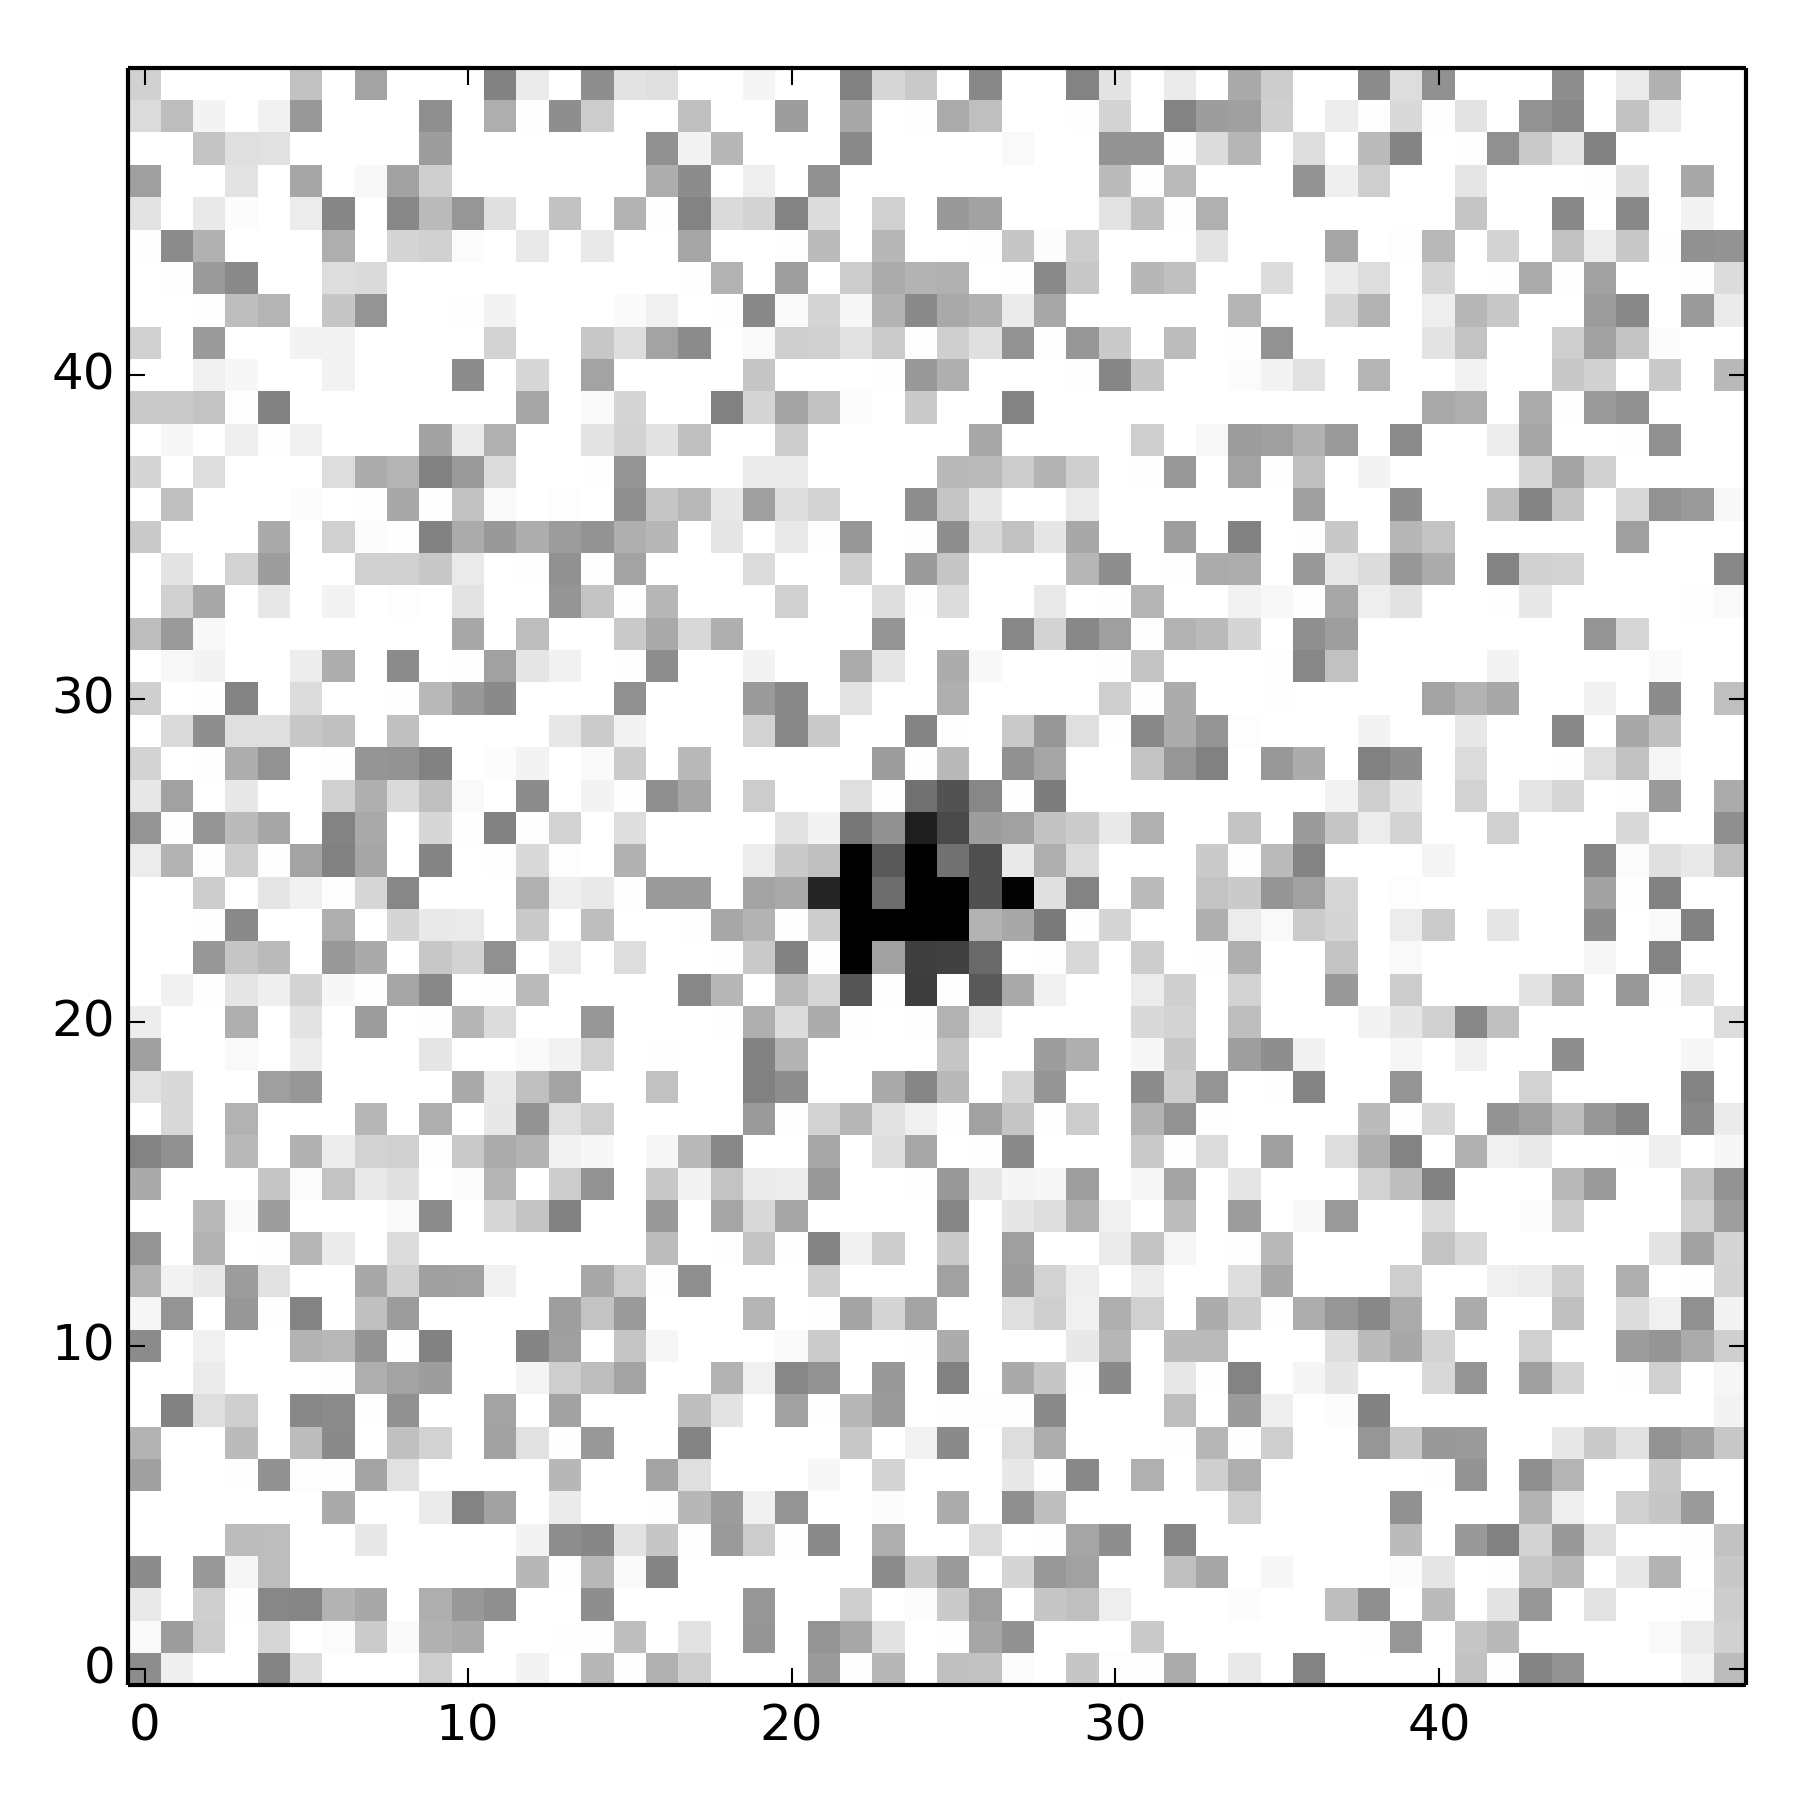
\includegraphics[width=\textwidth]{figures/golfholedata.png}
        \caption{$A_\text{data}$, $r=3$.
            \label{fig:golfhole_data}
        }
    \end{subfigure}

    \begin{subfigure}[b]{0.7\textwidth}
            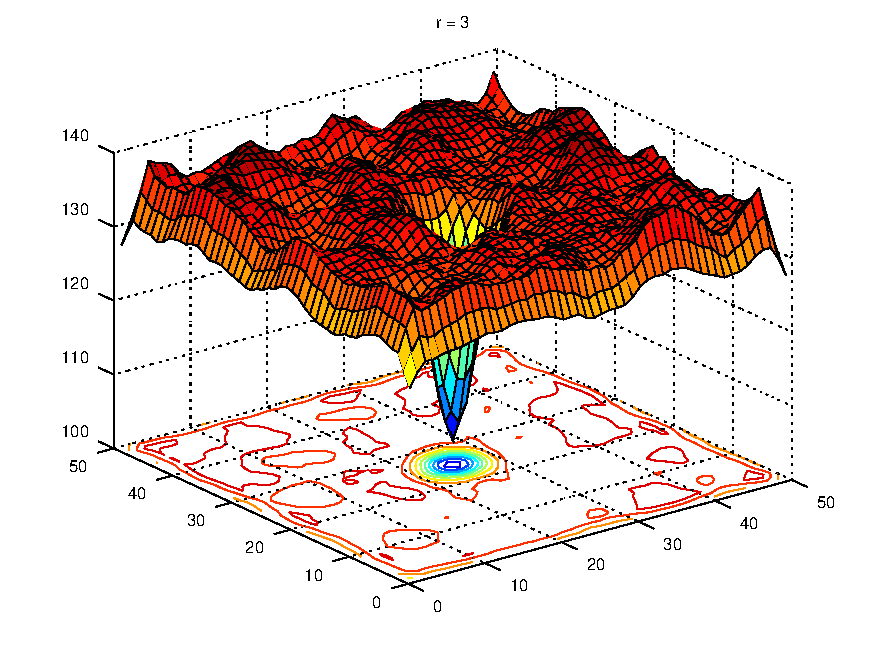
\includegraphics[width=\textwidth]{figures/golfhole2.pdf}
        \caption{Kiinteä $r=3$. 
            \label{fig:golfhole2}
        }
    \end{subfigure}

    \begin{subfigure}[b]{0.7\textwidth}
            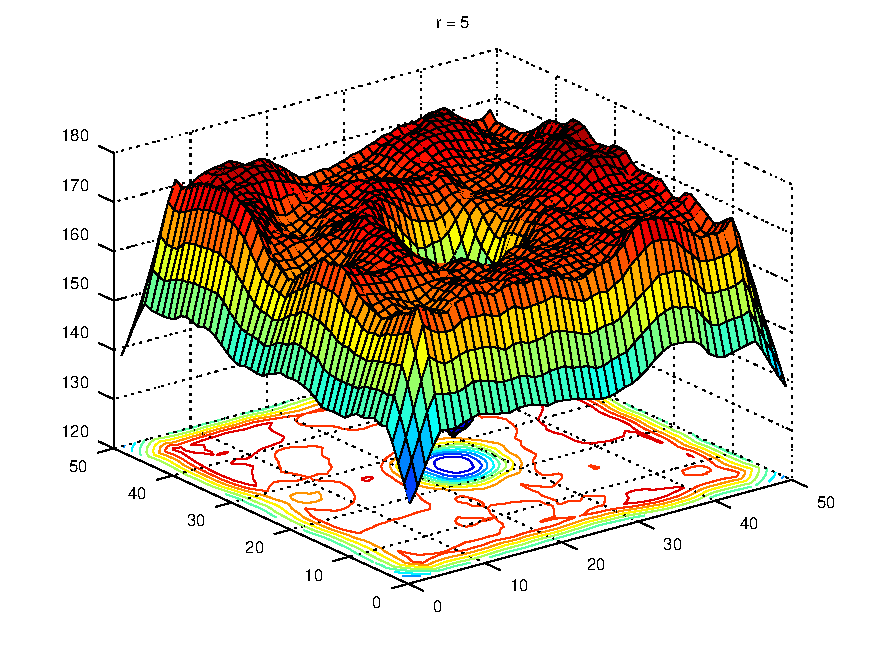
\includegraphics[width=\textwidth]{figures/golfhole3.pdf}
        \caption{Kiinteä $r=5$.
            \label{fig:golfhole3}
        }
    \end{subfigure}
    \caption{Energiafunktion $E_\text{naiivi}$ energiamaasto $xy$-avaruudessa.
        Energiamaasto on $xy$-ulottuvuudessa golf-reikämäinen (kuva~\ref{fig:golfhole2}), mutta $r$-ulottuvuudessa globaalin minimin 'kuoppa' näkyy alati laajemmalla alueella kun $r$ kasvaa.
        Huomaa myös reunojen lokaalit minimit.
        \label{fig:golfholes}}
\end{figure}


\begin{figure}[p]
    \centering
    \begin{subfigure}[b]{0.3\textwidth}
        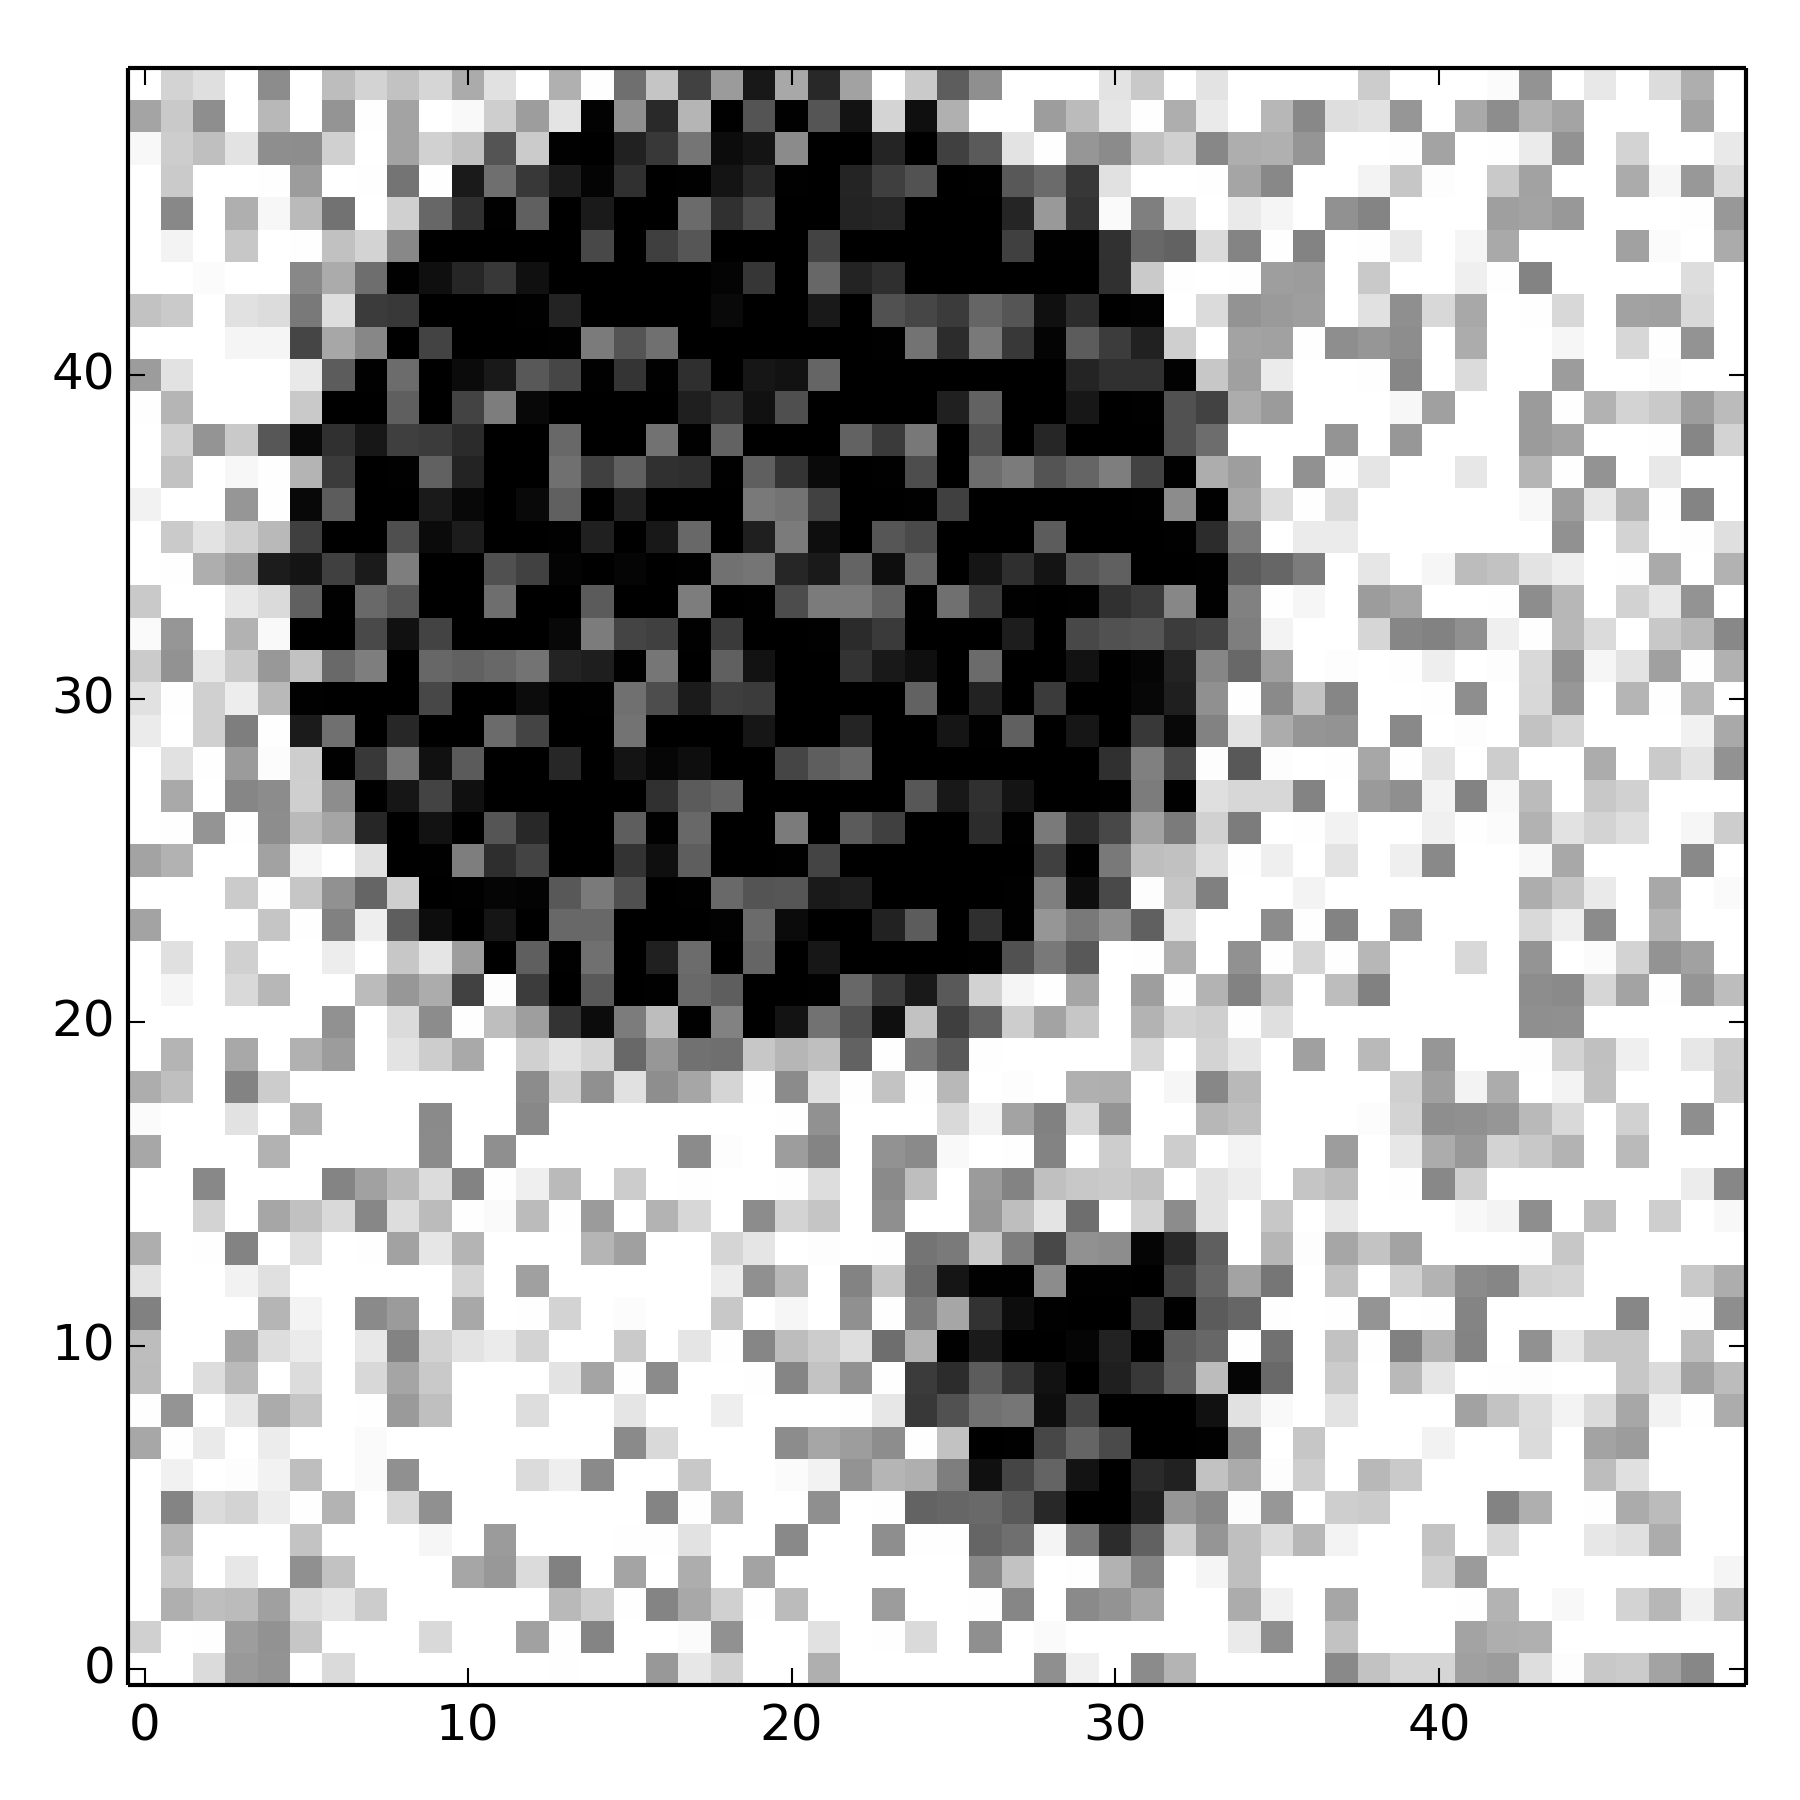
\includegraphics[width=\textwidth]{figures/localmindata.png}
        \caption{$A_\text{data}$. $(x_i,y_i,r_i) = (35, 20, 15), (10, 30, 5)$.
            \label{fig:localmin_data}
        }
    \end{subfigure}

    \begin{subfigure}[b]{0.7\textwidth}
            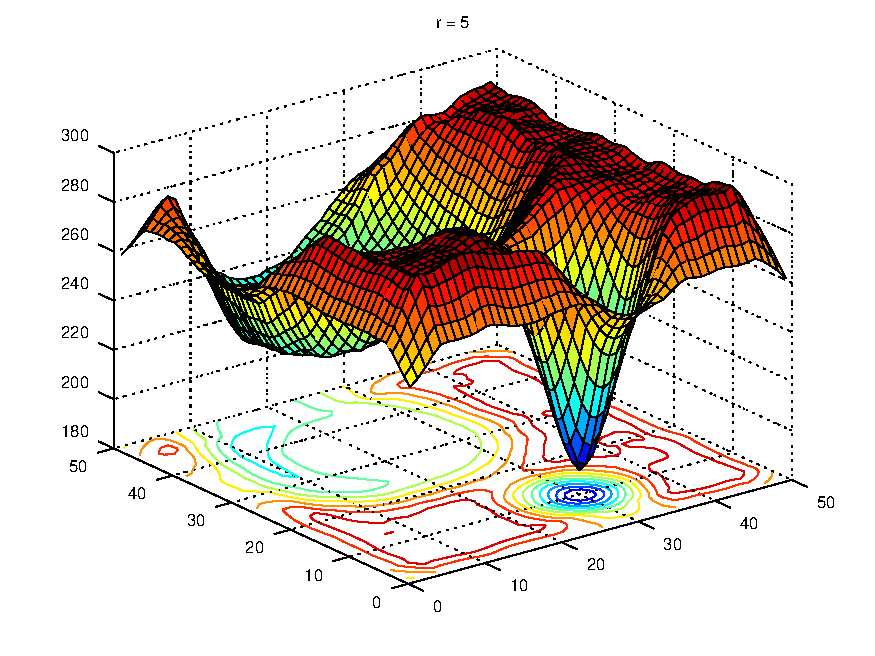
\includegraphics[width=\textwidth]{figures/localmins2.pdf}
        \caption{
            $E_\text{naiivi}$.
            \label{fig:localmins2}
        }
    \end{subfigure}

    \begin{subfigure}[b]{0.7\textwidth}
            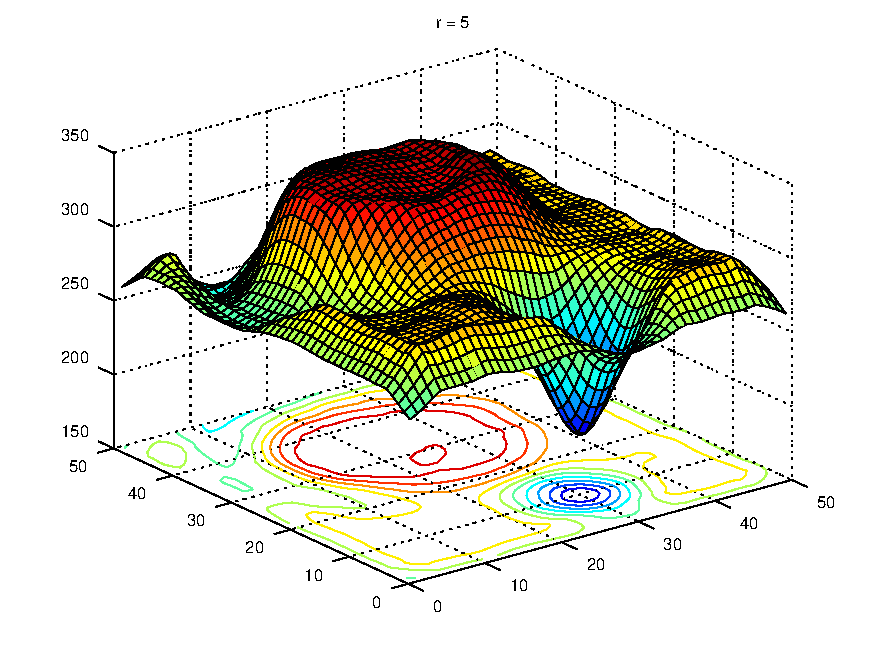
\includegraphics[width=\textwidth]{figures/localmins4.pdf}
        \caption{$E_\text{sov}$
            \label{fig:localmins4}
        }
    \end{subfigure}
    \caption{Energiafunktioiden $E_\text{naiivi}$ ja $E_\text{sov}$ arvoja toisen kiekon $x_2 y_2$-avaruudessa kun toisen kiekon säde $r_2=5$ ja ensimmäisen kiekon parametrit pidetään vakioina $(x_1, y_1, r_1) = (34, 22, 14)$.
        $E_\text{sov}$ rankaisee tiloista, joissa toinen parametrikiekko on ensimmäisen päällä.
        \label{fig:localmins}}
\end{figure}


\section{Siirtymät}
\label{sec:siirtymat}

Yksinkertaisin tapa toteuttaa jäähdytysalgoritmin 'pieni satunnainen siirtymä' olisi satunnaisesti valita jokin muuttujista $x, y, r$ ja lisätä tai vähentää siitä jokin kiinteä, pieni luku $\delta > 0$.
Käytännössä näin saataisiin jatkuvan parametriavaruuden $\Omega$ diskretisointi.
Tällöin kuitenkin joko menetettäisiin ratkaisutarkkuutta (jos $\delta$ on suuri) tai pienellä vakion arvolla $\delta \approx \text{pikseli}$ siirtymät olisivat liian pieniä jotta algoritmi kävisi ratkaisuavaruutta läpi tehokkaasti.

Tämän vuoksi käytetään seuraavaa menetelmää siirtymien generointiin:
Valitaan satunnainen kiekko, jonka parametrit ovat $(x, y, r)$.
Uusi piste $(x',y',r')$ valitaan $(x, y, r)$ -keskisen 'ellipsoidin' sisältä parametriavaruudessa $\Omega$:
\begin{align}
    r' &= \delta \cdot r, \qquad \delta \sim U(-1, 1),\\
    (x', y') &= (x, y) + \delta \cdot (\cos(\phi), \sin(\phi)), \qquad \phi \in U(0, 2\pi).
\end{align}

Lisäksi rajoitetaan $x,y$-siirtymiä siten ettei kiekon keskipiste voi mennä kuva-alueen $A$ ulkopuolelle.
Vastaavasti estetään arvot $r < 1$ pikseli ($r = 0$ muodostaisi myös lokaalin minimin) ja $r >$ kuvan koko.


\section{Jäähdytysstrategia}
\label{sec:jaahdytysstrategia}


SA-algoritmin jäähdytysstrategian valitsemiseen yleisesti kirjallisuus (\cite{laarhoven}, \cite{salamonetal}, \cite{recipes07}) tarjoaa lukuisia hyvin erilaisia vaihtoehtoja.
Tässä tutkielmassa käytetään yksinkertaista eksponentiaalista jäähdytysstrategiaa.

\subsection{Lämpötilan laskeminen}
\label{sub:lampotilan_laskeminen}

Lämpötilaa homogeenilla ketjulla $k$ päivitetään yhtälön
\begin{equation}
    t_{k+1} = \alpha \cdot t_k, \qquad k = 0, 1, 2, \dots
\end{equation}
mukaisesti,
missä $\alpha$ on vakio $1 - \epsilon$ jollekin pienelle $\epsilon >0$.
(Käytännössä 'pienellä' tarkoitamme että kokeilemme luvussa~\ref{cha:tulokset} arvoja $\alpha = 0.90 \dots 0.99$.)

Markov-ketjun pituus kullakin kontrolliparametrin arvolla $t_k$ asetetaan vakioksi $L_k = 10$.


\subsection{Lämpötilan alkuarvo}
\label{sub:lampotilan_alkuarvo}

Kontrolliparametrin alkuarvo $t_0$ eli lähtölämpötila pyritään valitsemaan siten,
että lämpötilan ensimmäisillä arvoilla hyväksyttyjen tilamuutosten suhde kaikkiin yritettyihin  tilamuutoksiin  $q$ on lähellä yhtä, eli
\begin{equation}
    \label{eq:ratio}
    q_0 = \exp{-\mean{\Delta E} / t_0} \approx 1,
\end{equation}
missä $\mean{\Delta E}$ on 'keskimääräistä' satunnaista siirtymää vastaava energiafunktion muutos lämpötilassa $t_0$.
Toisaalta ei ole toivottavaa, että $t$ säilyy korkeana (ja $q \approx 1$) \emph{liian} pitkään, jolloin siitä ei enää hyötyä algoritmin toimivuuden kannalta ja simulointi korkeissa lämpötiloissa vie turhaan laskenta-aikaa.

Näin ollen kunkin algoritmin ajokerran alussa valitaan sopiva arvio saadaan yhtälön~\ref{eq:ratio} avulla:
\begin{align}
    \exp\left(-\mean{\Delta E} / t_0\right) &= q_0 \quad (\leq 1)\\
    t_0 &= -\frac{\mean{\Delta E}}{\log{q_0}}, \quad q_0 \leq 1,
\end{align}
missä keskimääräistä energiafunktion muutosta $\mean{\Delta E}$ kullakin $A_\text{data}$ arvioidaan simuloimalla muutamia jaksossa~\ref{sec:siirtymat} kuvailtuja siirtymiä.

\subsection{Loppukriteeri}
\label{sub:loppukriteeri}

Käytännön varotoimenpiteenä asetetaan maksimiraja kuinka monta iteraatiota algoritmia suoritetaan ($n = 1000$ homogeenia 10 iteraation Markov-ketjua).

Varsinaiseksi lopetuskriteeriksi asetamme kuitenkin sen lämpötilan, jossa Markov-ketjut alkavat toistua samankaltaisina,
eli uudet iteraatiot pienemmillä lämpötiloilla eivät enää vaikuta johtavan merkittävästi parempiin ratkaisuihin.
Käytännössä kelvolliseksi osoittautui katkaisuehto,
jossa algoritmin iteraatio $i$ jää viimeiseksi $i := i_\text{final}$, jos
\begin{equation}
    \frac{\sum_{j=0,\dots,3} q_{i-j}}{4} < 0.05.
\end{equation}





    \chapter{Tulokset}
\label{cha:tulokset}

\section{Testiaineisto}
\label{sec:testiaineisto}

Algoritmin tutkimista varten luotiin simuloitu testiaineisto jaksossa~\ref{sec:simuloitu_aineisto} kuvaillun mallin mukaisesti.
Aineistoa varten generoitiin suuri joukko erilaisia parametreiltaan mielivaltaisten $k = 1, ..., 5$ kiekon harmaasävykuvia,
joiden koko oli $50 \times 50$ pikseliä,
ja algoritmin toiminnan tarkastelua varten poimittiin esimerkinluontoisesti kuusi kuvaa (a, b, c, d, e, f), jotka näkyvät kuvassa~\ref{fig:all_datasets}.
Testikuvien a, b, ja c avulla esitellään algoritmin toimintaa kiekkomäärän kasvaessa.
Kuvan d avulla taas vaikuttavatko eri jäähdytysskenaariot ratkaisun tarkkuuteen löytää pieni kiekko ($x = 35, y = 35, r = 2$),
ja testikuvia e, f vertailemalla tarkastellaan miten yhden kiekon säteen muutos algoritmin toimintaan.

\begin{figure}[htb]
    \centering
    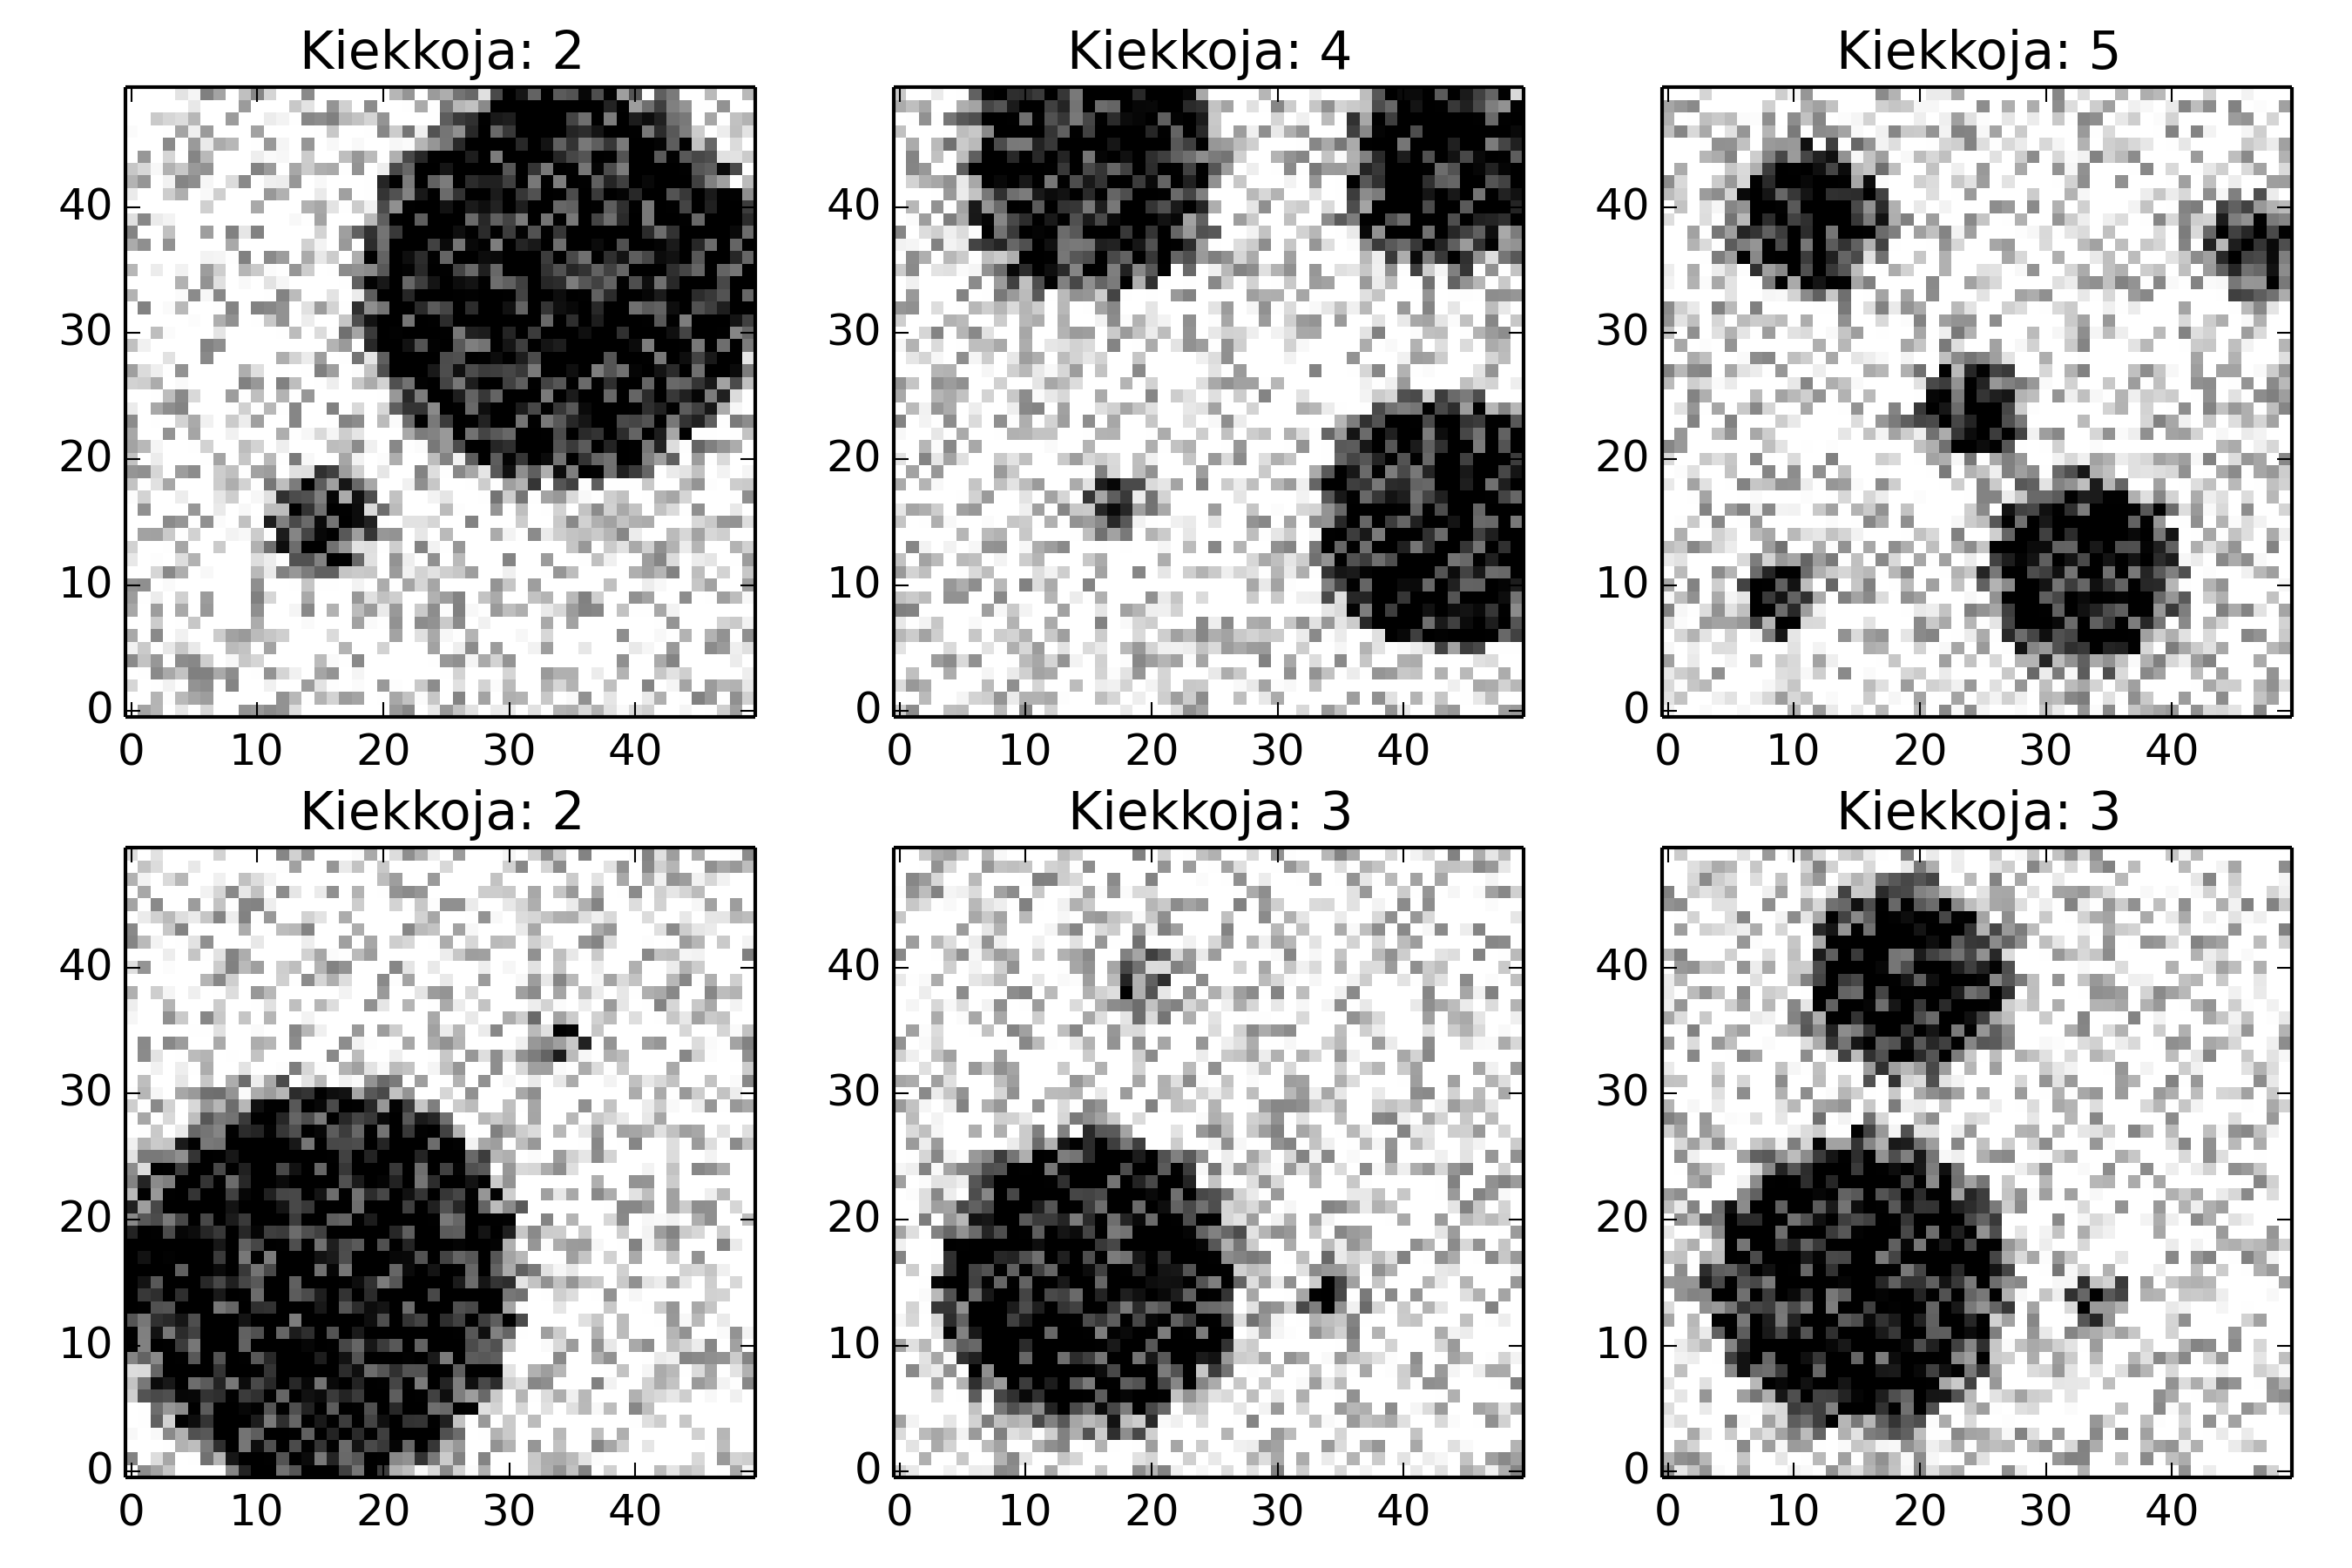
\includegraphics[width=\linewidth]{figures/all_datasets.png}
    \caption{Tutkielmassa lähemmin tarkasteltavat testikuvat.
        Vasemmalta oikealle, ylärivi: Testikuvat a, b, c.
        Alarivi: d, e, f.
    \label{fig:all_datasets}}
\end{figure}

\section{Ratkaisun onnistumisen mittaaminen}
\label{sec:ratkaisun_onnistumisen_mittaaminen}

Kuvaillaan vielä mitat, joita käytetään ratkaisun onnistumisen arvioimiseen.

\subsection{Energiafunktio}
\label{sub:energiafunktio}

Energiafunktion arvon tarkastelu kullakin iteraatiolla kunkin kulkijan edetessä on luonnollinen menetelmä arvioida optimointialgoritmin toimintaa.
Varjopuolena kuva energiafunktion tarkastelu ei välttämättä kerro paljonkaan kuinka hyvä ratkaisu on tarkasteltavan kuvakäsittelyongelman suhteen.

\subsection{Pinta-alan symmetrinen erotus}
\label{sub:pinta_alan_symmetrinen_erotus}

Toinen vaihtoeheto on verrata todellisen ja ratkaisun kiekkojen symmetristä erotusta.
Olkoon $W_\text{final}$ kulkijan lopullinen ratkaisu ympyräparametreille ja $W_\text{orig}$ alkuperäiset datan luomiseen käytetyt kiekkojen parametrit,
ja $A_W$ luvun~\ref{cha:kuvamalli_ja_aineisto} mallin mukaisesti kiekkoparametreja vastaava häiriötön kuva jossa $A_{ij} = 0$, jos pikseli on kuvan sisällä.
Olkoon myös vastaava kuvaa $A$ vastaava käänteiskuva $A' = 1 - A$ kuten kappaleessa~\ref{sub:paranneltu_monen_kiekon_energiafunktio}.
Tälloin symmetriseen erotukseen perustuva mitta on
\begin{equation*}
    m_\text{symm}(W_\text{final}, W_\text{orig}) = (A_{W_\text{final}}' \setminus A_{W_\text{orig}}') \cup (A_{W_\text{orig}}' \setminus A_{W_\text{final}}'),
\end{equation*}
kun kuvamatriisit mielletään joukoiksi, johon joku tietty pikseli kuuluu ($A_{ij}' = 1$) tai ei ($A_{ij}' = 0$).
Mitta vastaa naiivia energiafunktiota ja melko samankaltainen parannellun energiafunktion kanssa.

\subsection{Sovellettu etäisyysmitta}
\label{sub:sovellettu_etaisyysmitta}

Määritellään lisäksi toisenlainen ratkaisukiekkojen etäisyyttä todellisista mittaava mitta joka ei perustu pinta-aloihin,
mutta kuitenkin vastaa intuitiivisista käsitystä kiekkojen etäisyydestä:
Valitaan löydetyn ratkaisun ja todellisten kiekkojen väliseksi etäisyydeksi summa kunkin ratkaisukiekon keskipisteen ja säteen Euklidinen etäisyys alkuperäisten kiekkojen keskipisteeseen ja säteeseen
kun ratkaisun kiekkojen todelliset vastineet valitaan kaikkien mahdollisten kiekkoparien etäisyyksien pienuusjärjestyksessä.

Toisin sanoen käytetään seuraavanlaista algoritmia.
Olkoon $W_\text{final}, W_\text{orig}$  kiekkojoukot kuten yllä, ja lasketaan etäisyys $m_\text{sov}$ seuraavasti:
\begin{algorithm}[h]
    \KwData{$W_\text{final}, W_\text{orig}$}
    \KwResult{$m_\text{sov}$}
    \BlankLine
    $n_\text{circles} \leftarrow \abs{W}$ \;
    $m_s \leftarrow 0$\;
    \For{$i \leftarrow 1$ \KwTo $n_\text{circles}$}{
        $d_\text{min} \leftarrow \min\limits_{a \in W_\text{final}, b \in W_\text{orig}} \norm{a.x - b.y} + \norm{a.y - b.y} + \norm{a.r - b.r}$\;
        $a_\text{min}, b_\text{min} \leftarrow \underset{a \in W_\text{final}, b \in W_\text{orig}}{\operatorname{argmin}} \norm{a.x - b.y} + \norm{a.y - b.y} + \norm{a.r - b.r}$\;
        $m_\text{sov} \leftarrow m_s + d_\text{min}$\;
        $W_\text{final} \leftarrow W_\text{final} \setminus a_\text{min}$\;
        $W_\text{orig} \leftarrow W_\text{orig} \setminus b_\text{min}$\;
    }
\end{algorithm}


\section{Algoritmin tulokset}
\label{sec:algoritmin_tulokset}

Testiaineiston kuville ajettiin 100 kertaa luvussa~\ref{cha:algoritmin_soveltaminen} kuvailtu algoritmi vaihtelevalla määrällä jäähdytysskenaarioita $\alpha = 0.90 \dots 0.99$.
Jokaista algoritmin ajokertaa tietyin parametrein eli toteutunutta Markov-ketjua nimitetään jatkossa \emph{kulkijaksi}.

Koska kulkijat ovat itsenäisiä, kunkin 100 kulkijan kokoelman simuloinnissa voitiin hyödyntää rinnakkaislaskentaa.
Numeeriseen laskentaan käytettiin Helsingin yliopiston Tietojenkäsittelytieteen laitoksen Ukko-laskentaklusteria.

\begin{table}[htpb]
    \centering
    \caption{Testiaineiston kuvat a, b, c. Kuvien~\ref{fig:A_datasets_res_fast} ja \ref{fig:A_datasets_res_slow} energiafunktion suhteen parhaiden ratkaisujen lopulliset energiat, virheet ja kulkijoiden pituus (homogeenien Markov-ketjujen määrä). Jäähdytysskenaariot $\alpha = 0.90$ ja $\alpha = 0.99$.
        \label{tab:A_res_fast_errors}
    }
    \begin{tabular}{l c c c c c}
        $\alpha$ & Aineisto & Markov-ketjuja & Energia & $m_\text{sov}$ & $m_\text{symm}$ \\[2pt]
        \hline\noalign{\smallskip}
        0.90 & a & 56 & 129.982734083 & 1.43765180533 & 22 \\
             & b & 52 & 136.670018567 & 3.36654077973 & 66 \\
             & c & 60 & 159.514844916 & 6.75832581266 & 131 \\[1pt]
        \hline\noalign{\smallskip}
        0.99 & a & 679 & 129.277573595 & 1.41934200707 & 22\\
             & b & 411 & 135.156720071 & 5.0613981837 & 49\\
             & c & 438 & 149.503374454 & 27.974956417 & 73
    \end{tabular}
\end{table}

\begin{figure}[htpb]
    \centering
    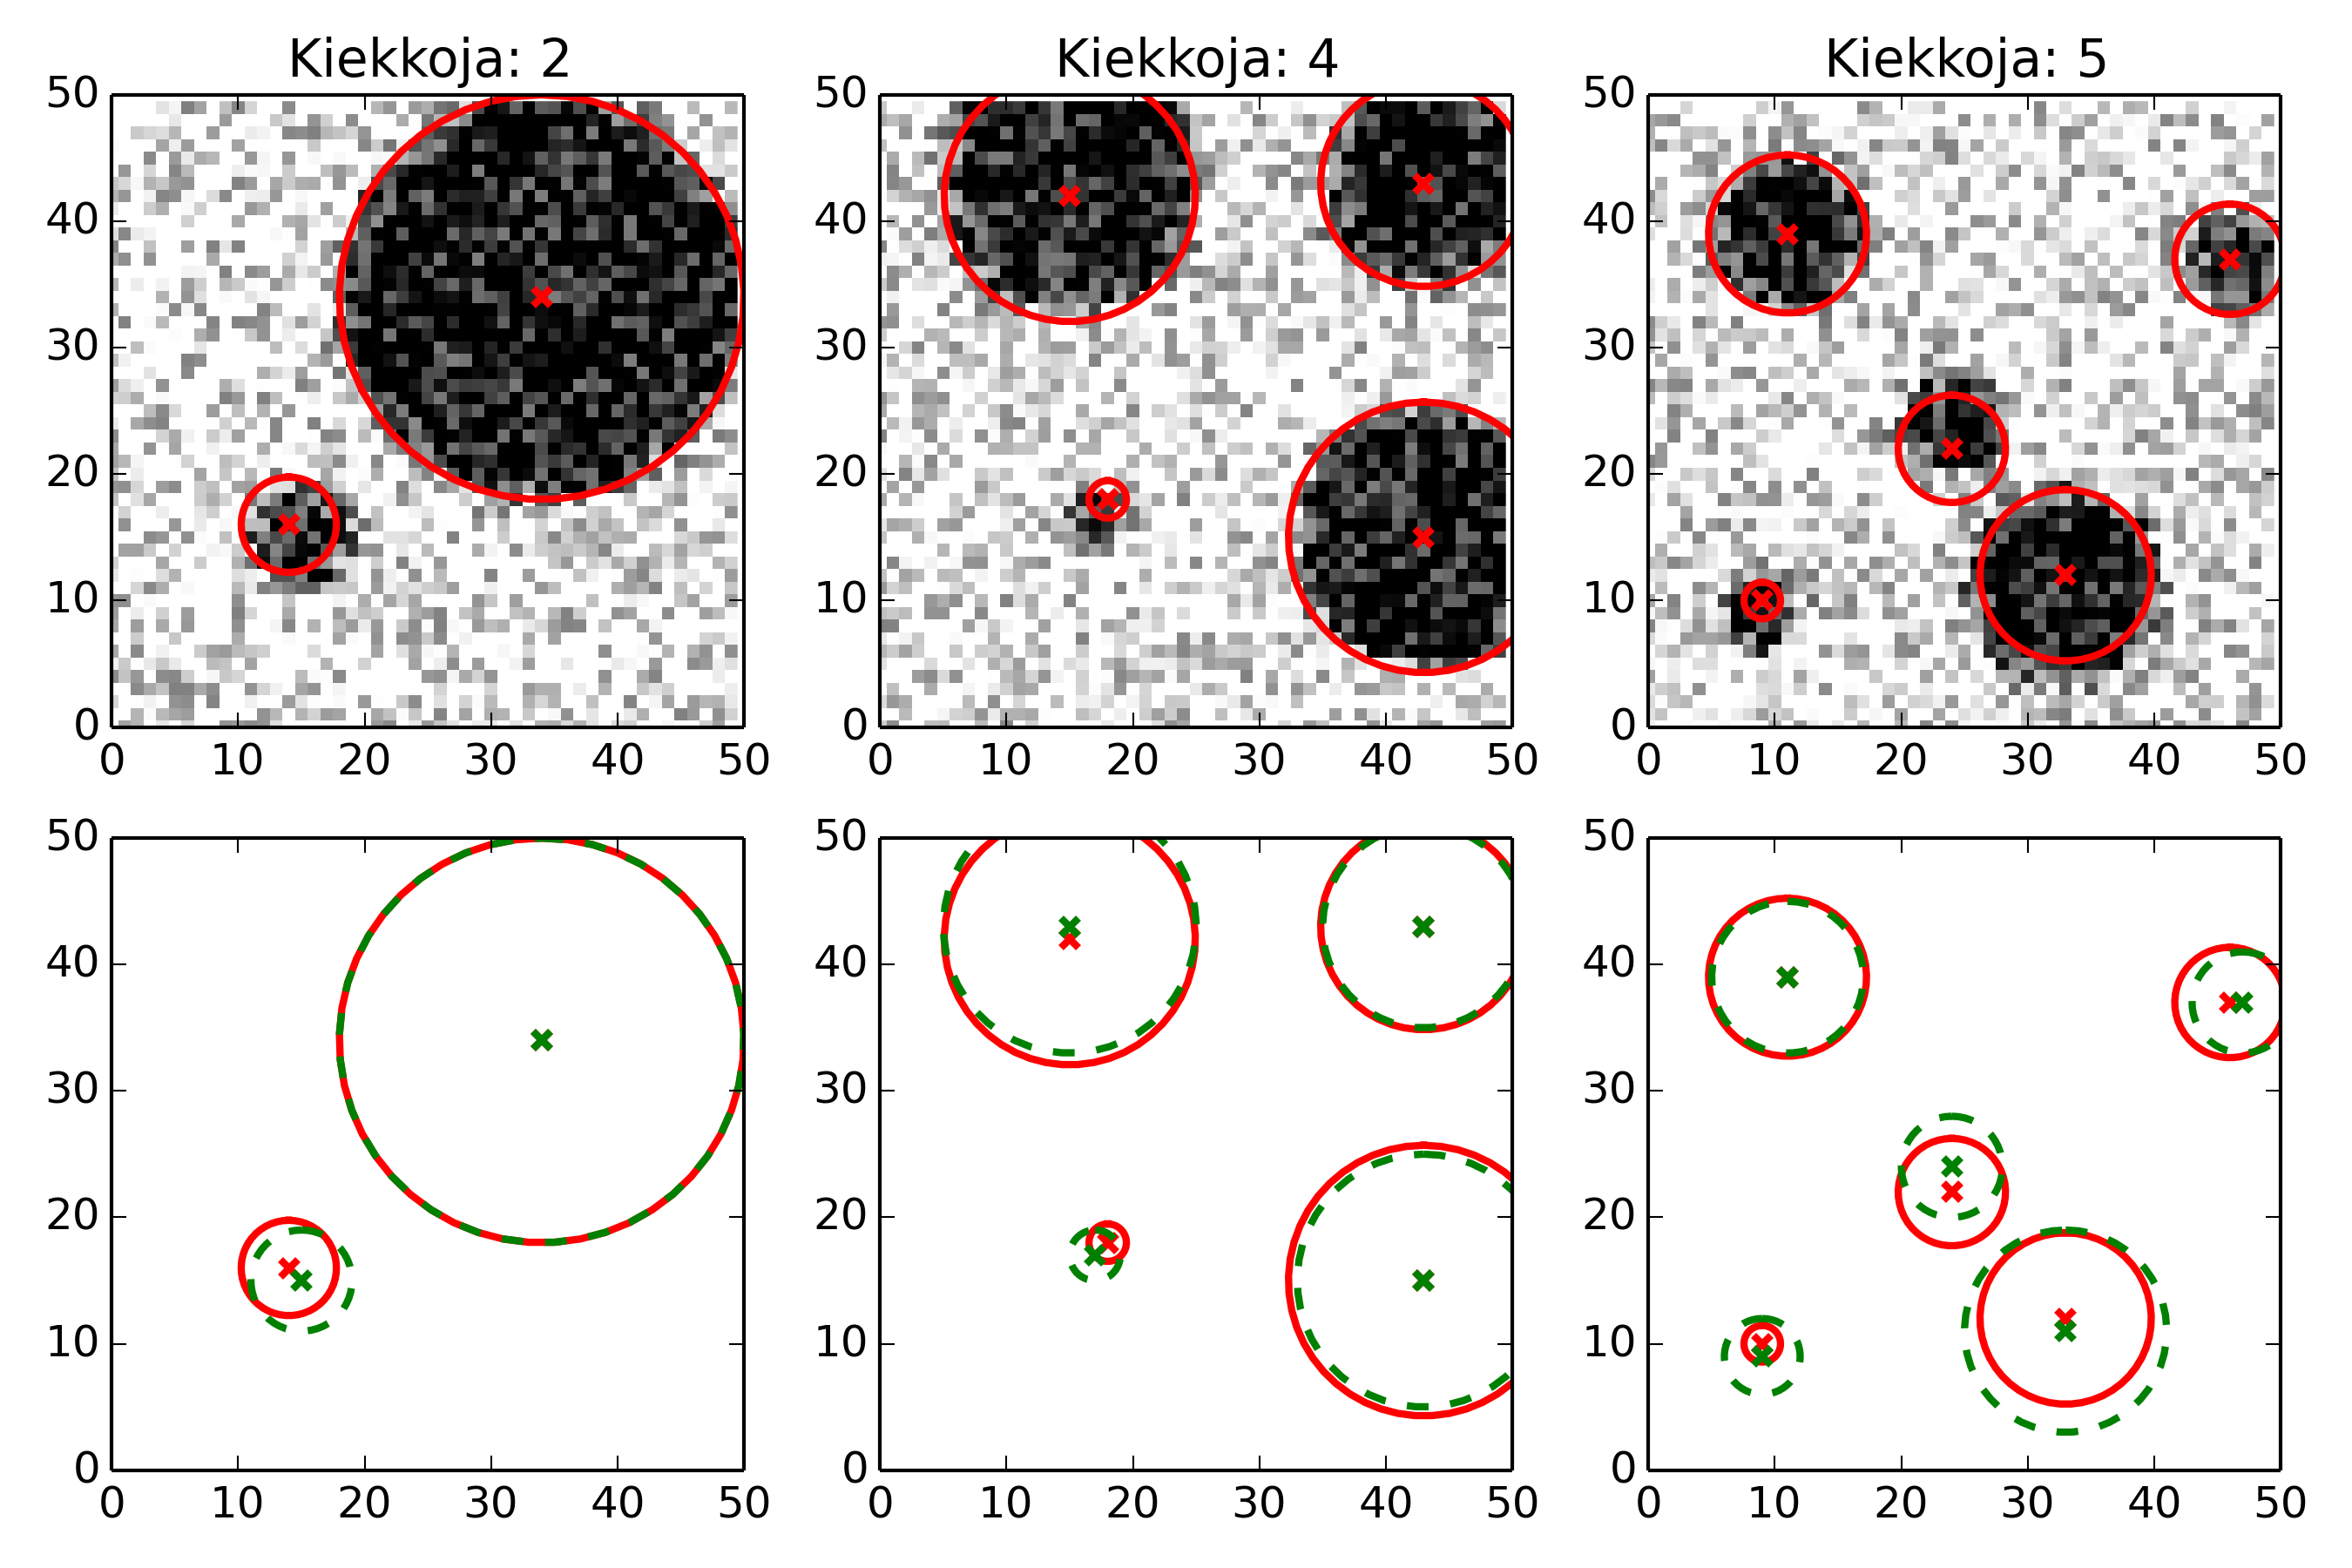
\includegraphics[width=1.0\linewidth]{figures/A_datasets_res_fast.png}
    \caption{Testiaineiston kuvat a, b, c: Parhaat ratkaisut energiafunktion suhteen (punaiset ympyrät) 100 kulkijan kokoelmasta jäähdytysskenaariolla $\alpha = 0.90$.
        Todelliset kiekot alarivillä vihreällä katkoviivalla.
        \label{fig:A_datasets_res_fast}
    }
\end{figure}


\begin{figure}[htpb]
    \centering
    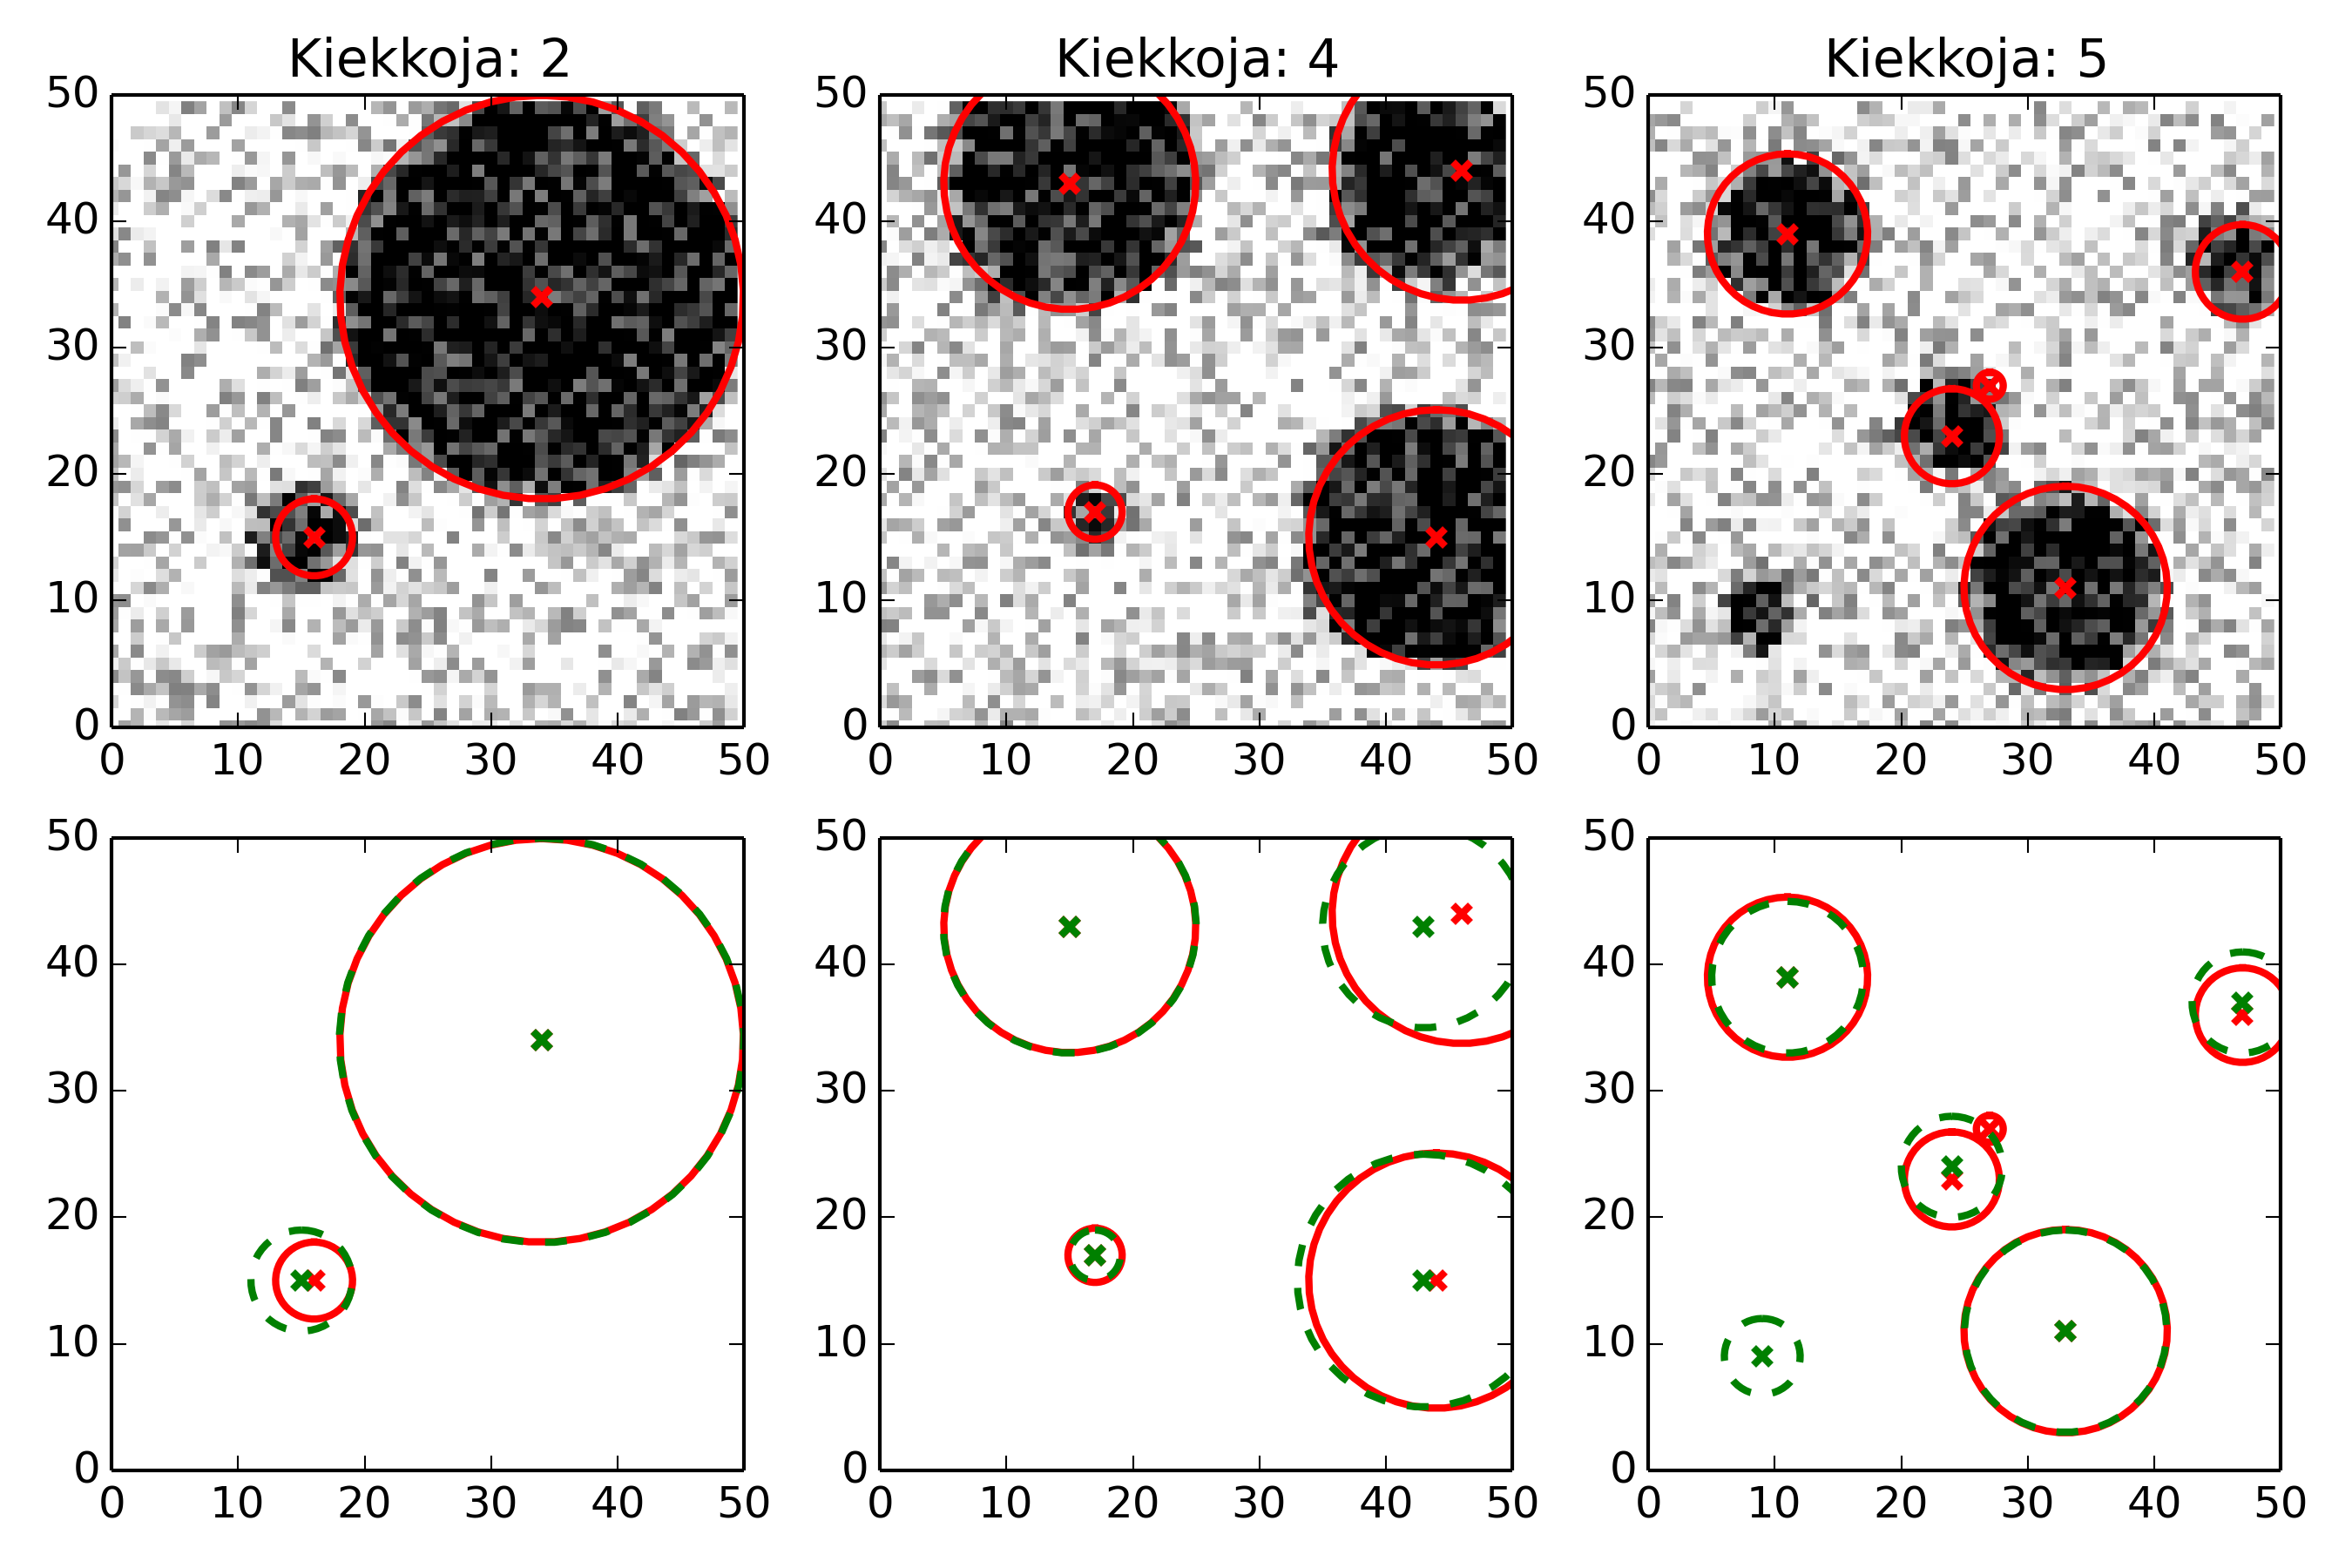
\includegraphics[width=1.0\linewidth]{figures/A_datasets_res_slow.png}
    \caption{Samat testikuvat a, b, c kuin kuvassa~\ref{fig:A_datasets_res_fast}: Parhaat ratkaisut energiafunktion suhteen (punaiset ympyrät) 100 kulkijan kokoelmasta jäähdytysskenaariolla $\alpha = 0.99$.
        \label{fig:A_datasets_res_slow}
    }
\end{figure}

\begin{figure}[htpb]
    \centering
    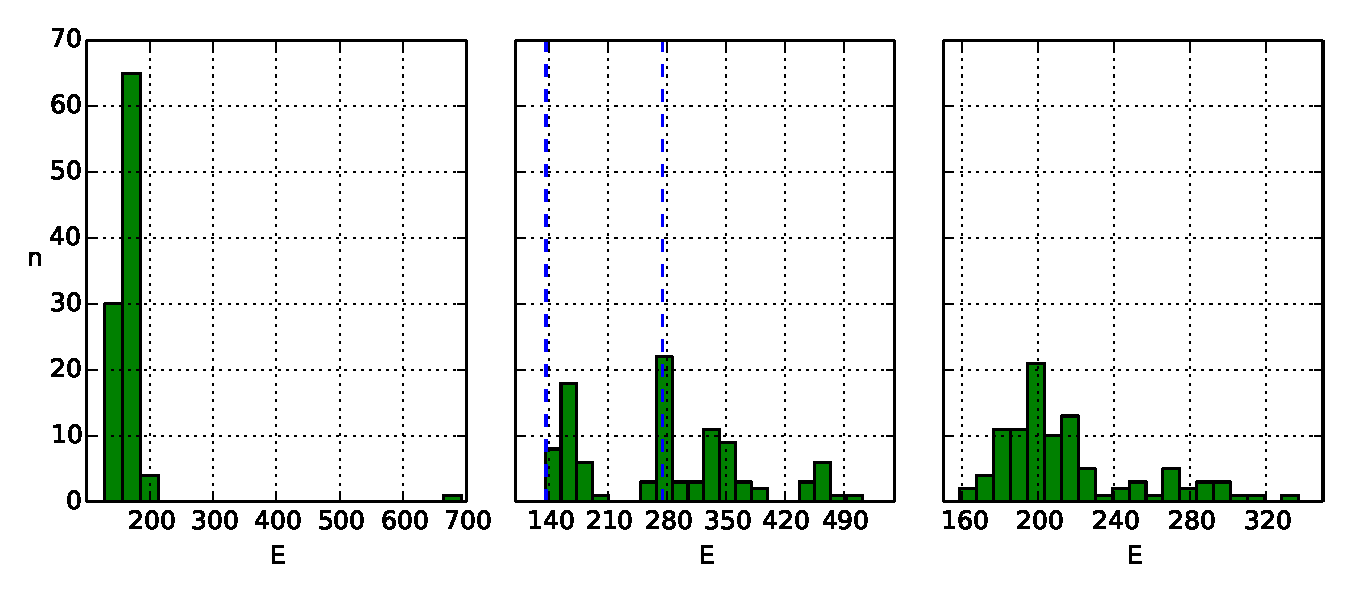
\includegraphics[width=1.0\linewidth]{figures/A_final_histo3_fast.pdf}
    \caption{Kuvan~\ref{fig:A_datasets_res_fast} skenaariota vastaavien kokoelmien kulkijoiden lopullisten energioiden jakaumat.
        Testikuvaa b vastaavaan histogrammiin merkitty kokoelman energialtaan paras ratkaisu sekä histogrammin moodi ($E \approx 280$).
        \label{fig:A_final_histo3_fast}
    }
\end{figure}


\begin{figure}[htpb]
    \centering
    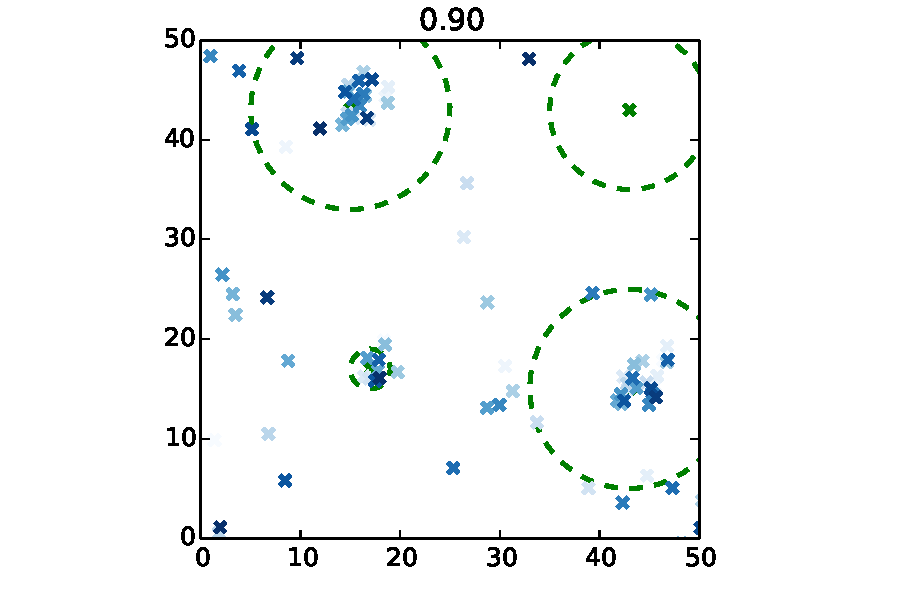
\includegraphics[width=1.0\linewidth]{figures/A_modalbin_cc_fast_1.pdf}
    \caption{Kuvan~\ref{fig:A_final_histo3_fast} testikuvan b histogrammin energiamoodin kulkijoiden ($n = 22$ kpl) löytämät keskipisteet, saman kulkijan pisteet samalla värillä.
        Keskipisteiden sijaintiin lisätty $U(-2,2)$-tärinää päällekkäisten merkkien näkemiseksi.
        Toisin kuin kuvassa~\ref{fig:A_final_histo3_fast} näkyvässä parhaassa ratkaisussa, loppuenergiamoodin kulkijat eivät näytä löytävän neljättä kiekkoa ($x = 44, y = 44, r = 8$).
        \label{fig:A_modalbin_cc_fast_1}
    }
\end{figure}

\begin{table}[htpb]
    \centering
    \caption{Testiaineiston kuva d. Kuvien~\ref{fig:set2_datasets_res_99} -- \ref{fig:set2_datasets_res_90} energiafunktion suhteen parhaiden ratkaisujen lopulliset energiat, virheet ja kulkijoiden pituus.
        \label{tab:2_res_errors}
    }
    \begin{tabular}{l c c c c c}
        Aineisto & $\alpha$ & Markov-ketjuja & Energia & $m_\text{sov}$ & $m_\text{symm}$ \\[2pt]
        \hline\noalign{\smallskip}
        d & 0.99 & 582 & 112.70531642  & 1.34903737042 & 12 \\
          & 0.98 & 292 & 115.799173967 & 17.1400032558 & 20 \\
          & 0.96 & 188 & 113.108609169 & 1.33302834307 & 12 \\
          & 0.94 & 103 & 112.772445287 & 1.3089734381  & 12 \\
          & 0.90 & 70  & 115.694414615 & 33.8856144998 & 22 \\
    \end{tabular}
\end{table}

\begin{figure}[p]
    \centering
    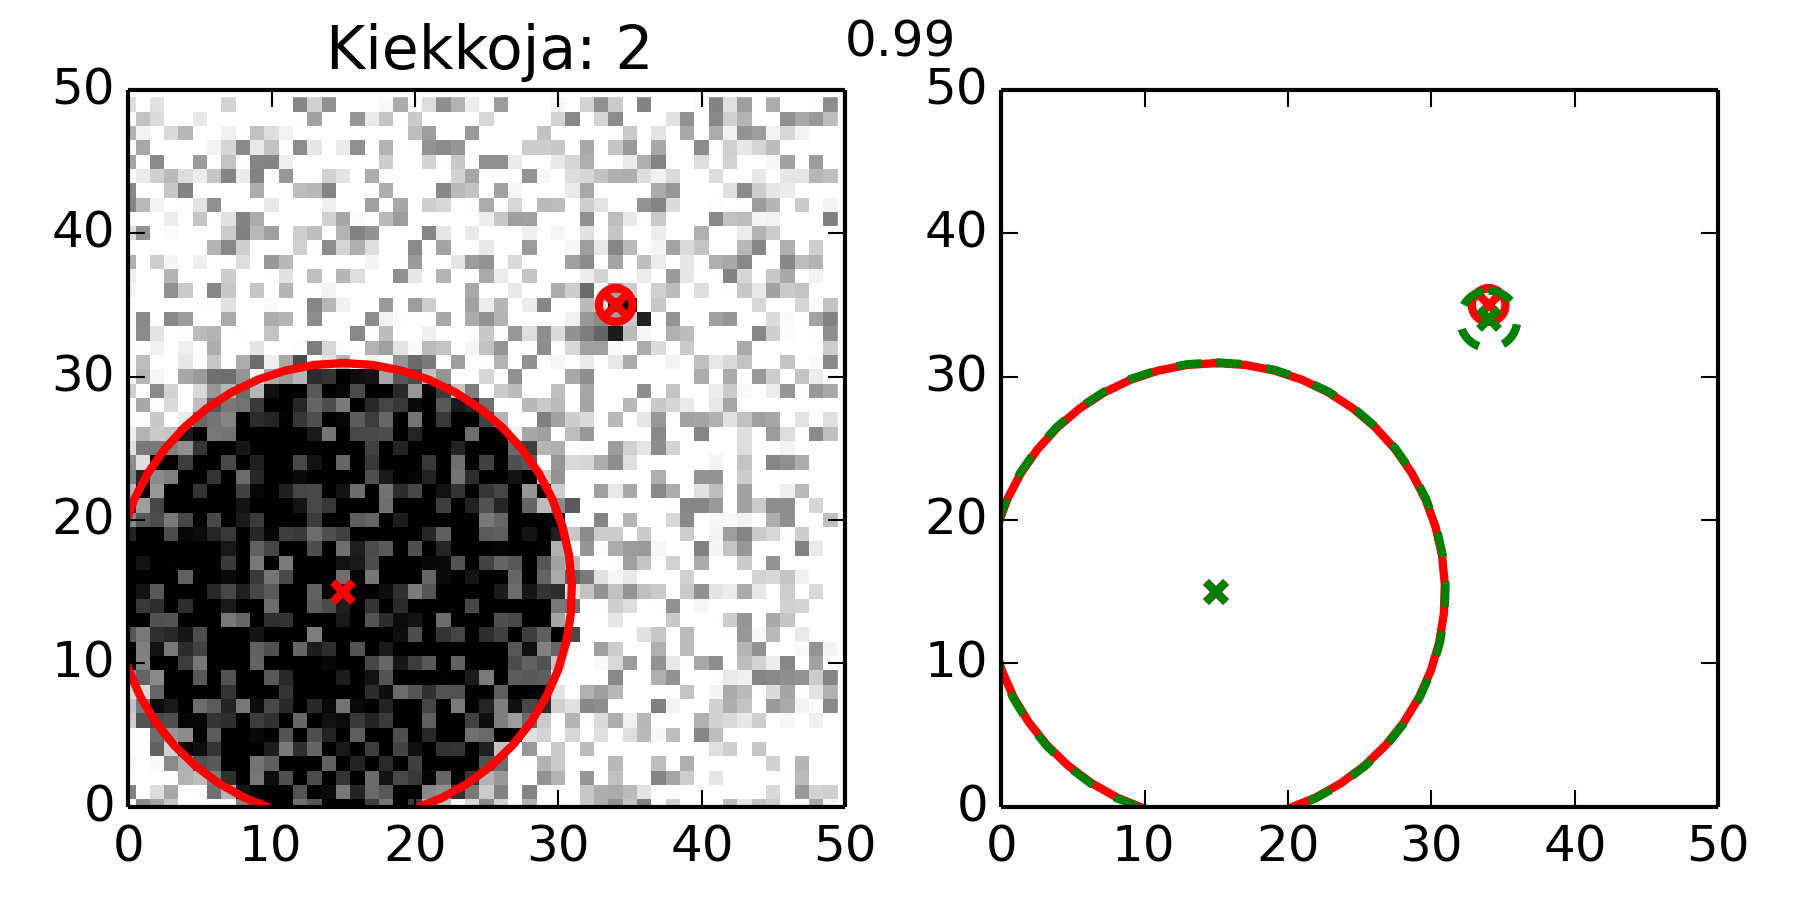
\includegraphics[width=0.7\linewidth]{figures/set2_datasets_res_99.png}
    \caption{Testikuva d, loppuenergialtaan paras kulkija 100 kulkijan kokoelmasta, kun $\alpha = 0.99$.
        \label{fig:set2_datasets_res_99}
    }
\end{figure}

\begin{figure}[p]
    \centering
    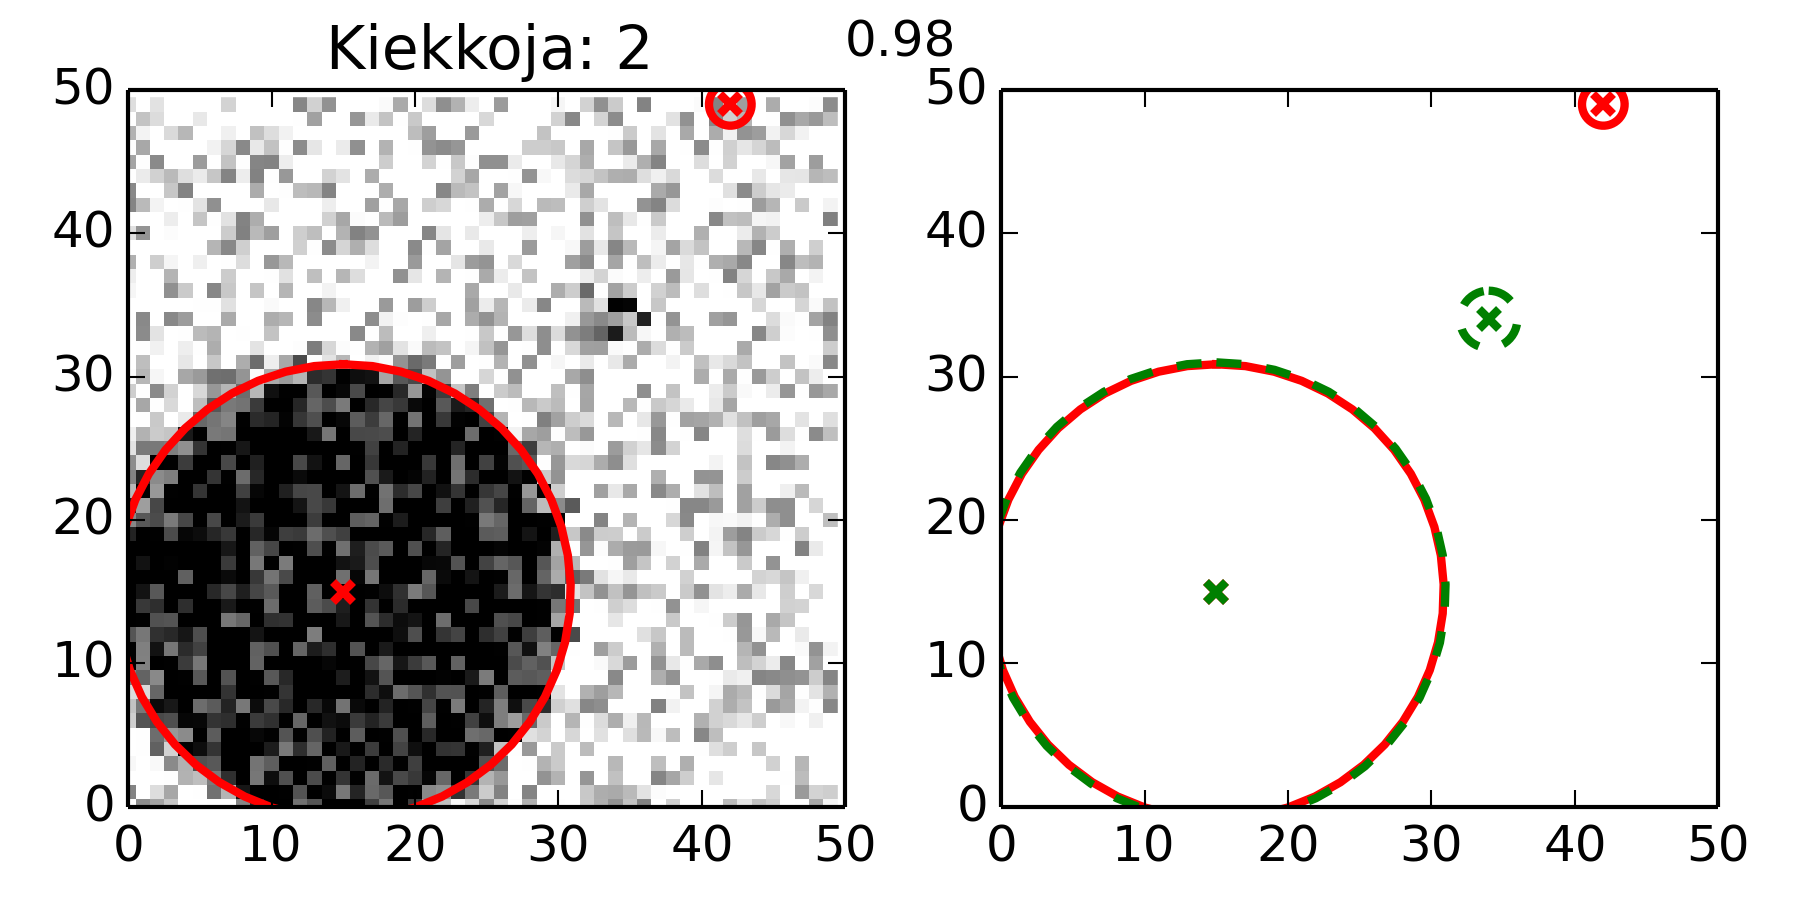
\includegraphics[width=0.7\linewidth]{figures/set2_datasets_res_98.png}
    \caption{Testikuva d. $\alpha = 0.98$.
        \label{fig:set2_datasets_res_98}
    }
\end{figure}


\begin{figure}[p]
    \centering
    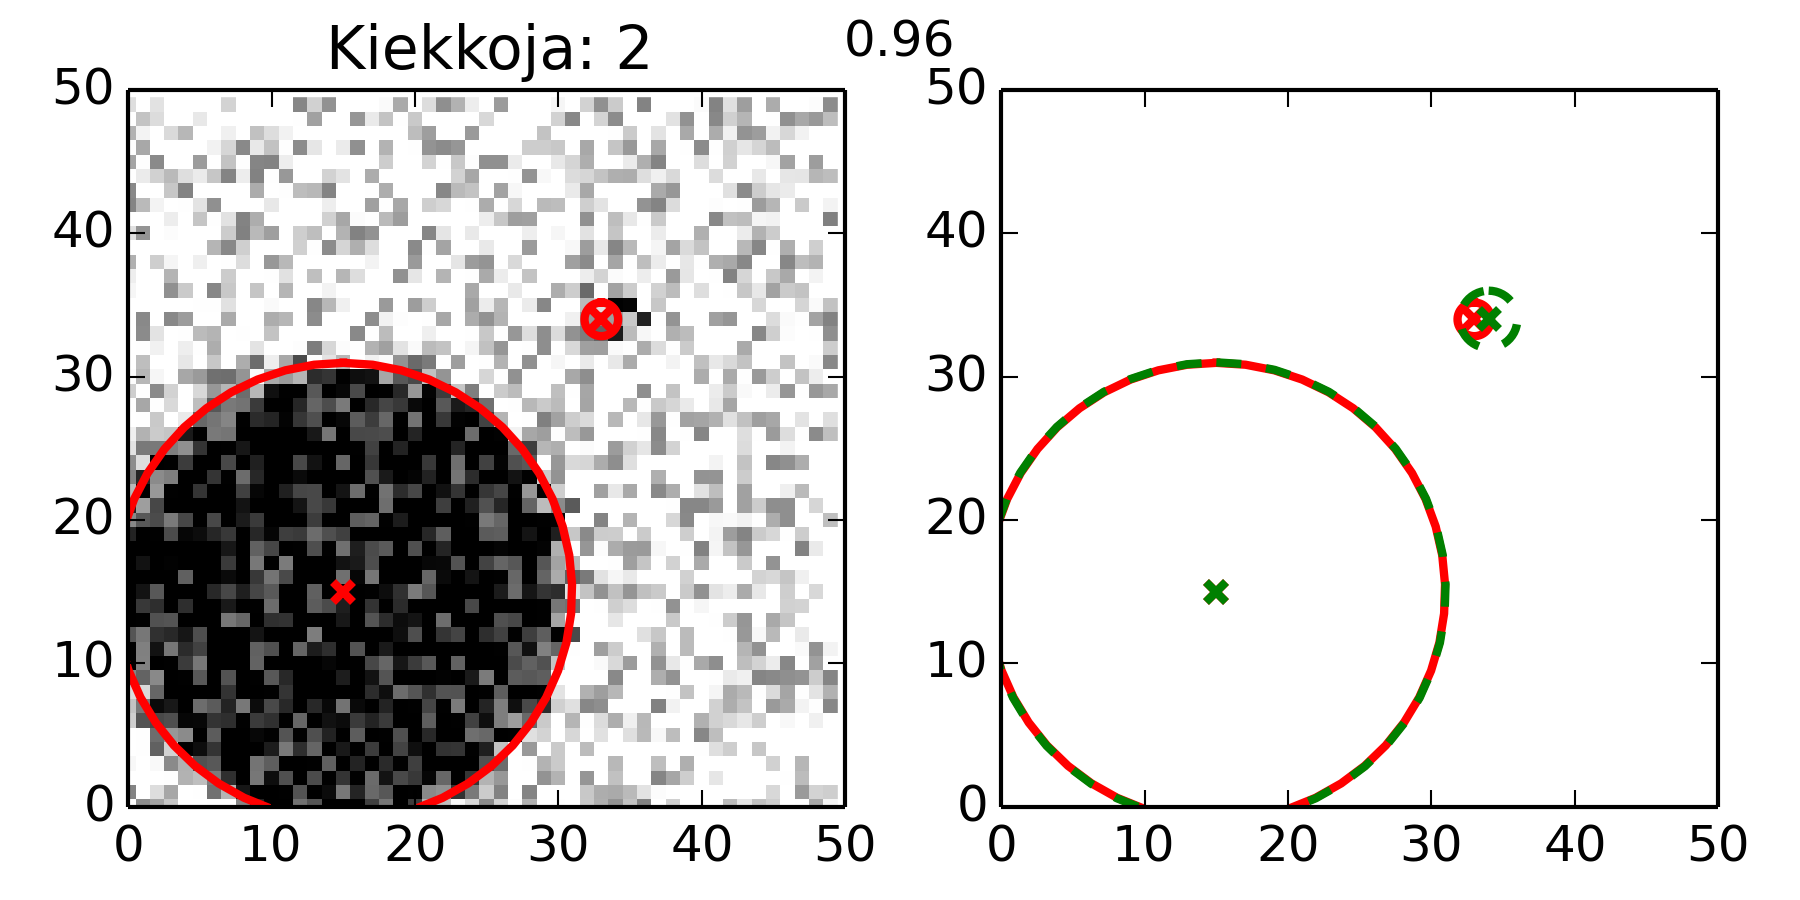
\includegraphics[width=0.7\linewidth]{figures/set2_datasets_res_96.png}
    \caption{Testikuva d. $\alpha = 0.96$.
        \label{fig:set2_datasets_res_96}
    }
\end{figure}


\begin{figure}[p]
    \centering
    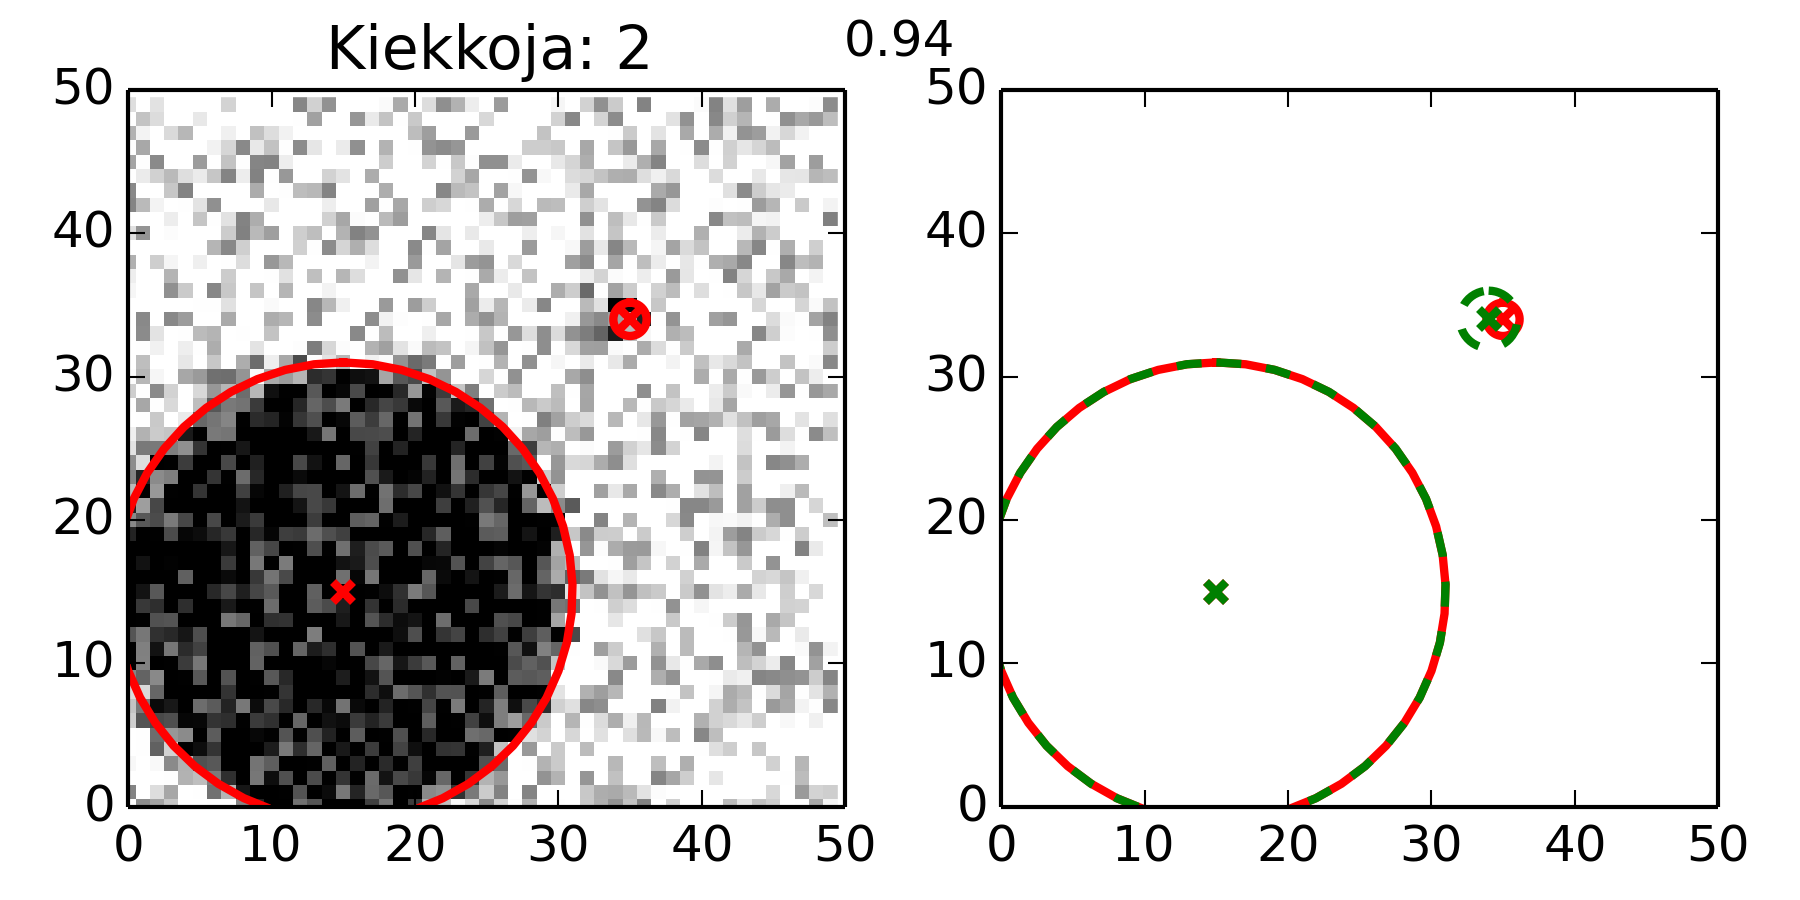
\includegraphics[width=0.7\linewidth]{figures/set2_datasets_res_94.png}
    \caption{Testikuva d. $\alpha = 0.94$.
        \label{fig:set2_datasets_res_94}
    }
\end{figure}


\begin{figure}[p]
    \centering
    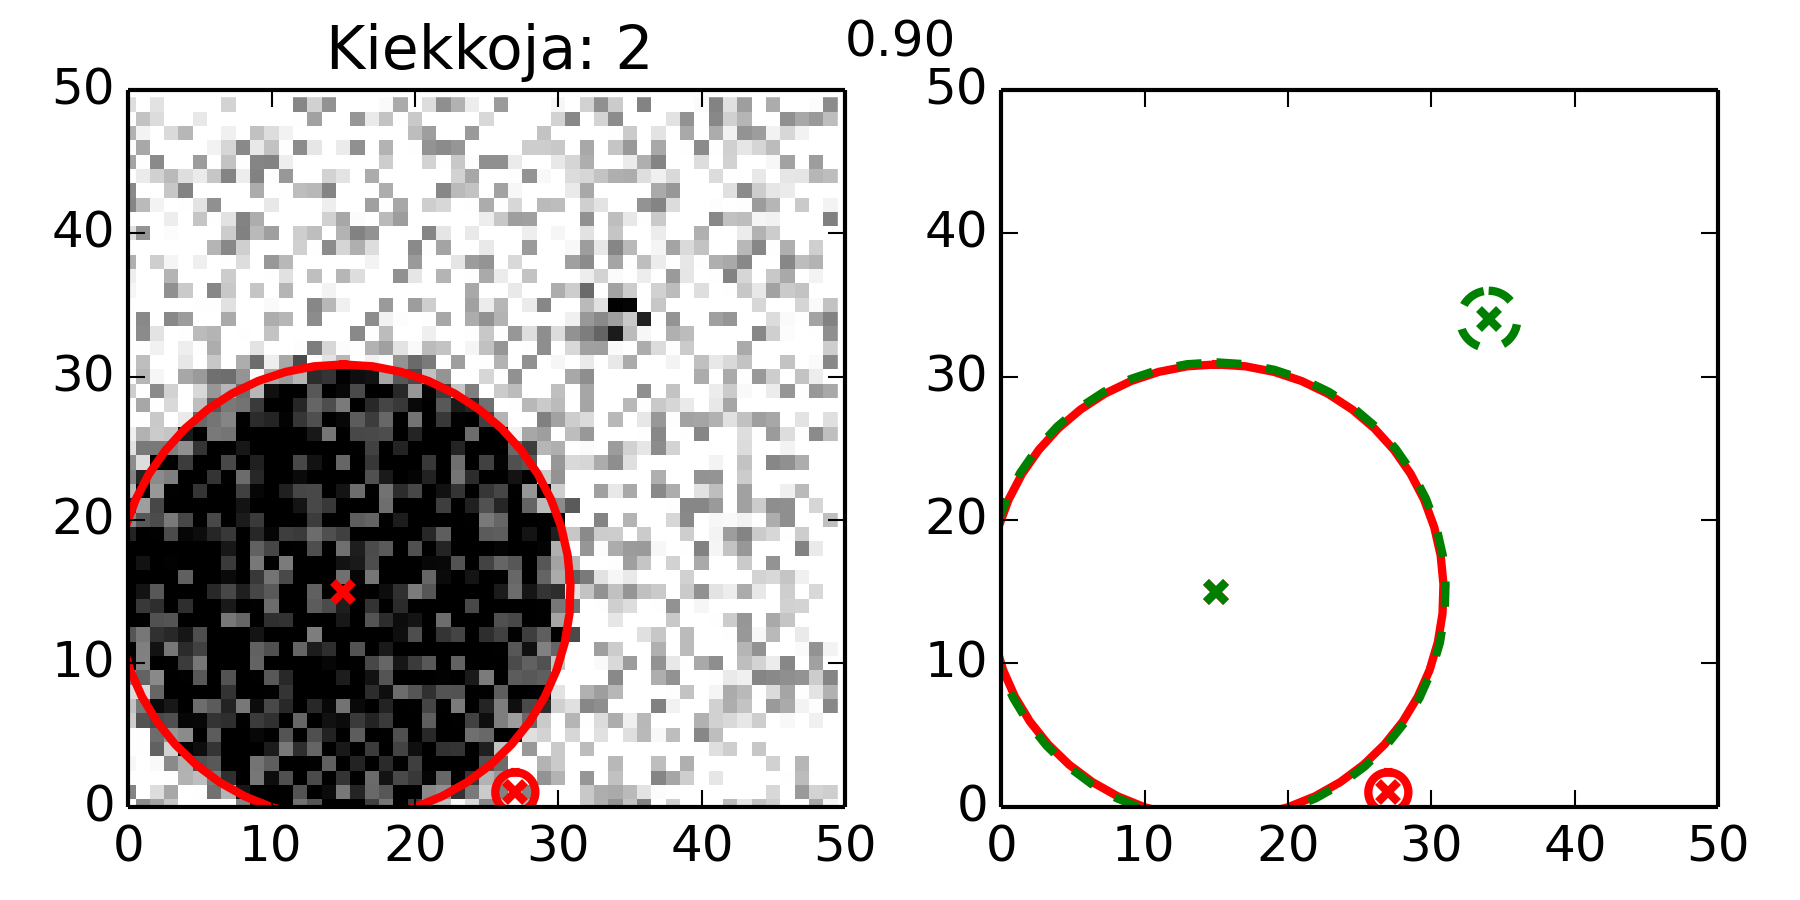
\includegraphics[width=0.7\linewidth]{figures/set2_datasets_res_90.png}
    \caption{Testikuva d. $\alpha = 0.90$.
        \label{fig:set2_datasets_res_90}
    }
\end{figure}

\begin{figure}[p]
    \centering
    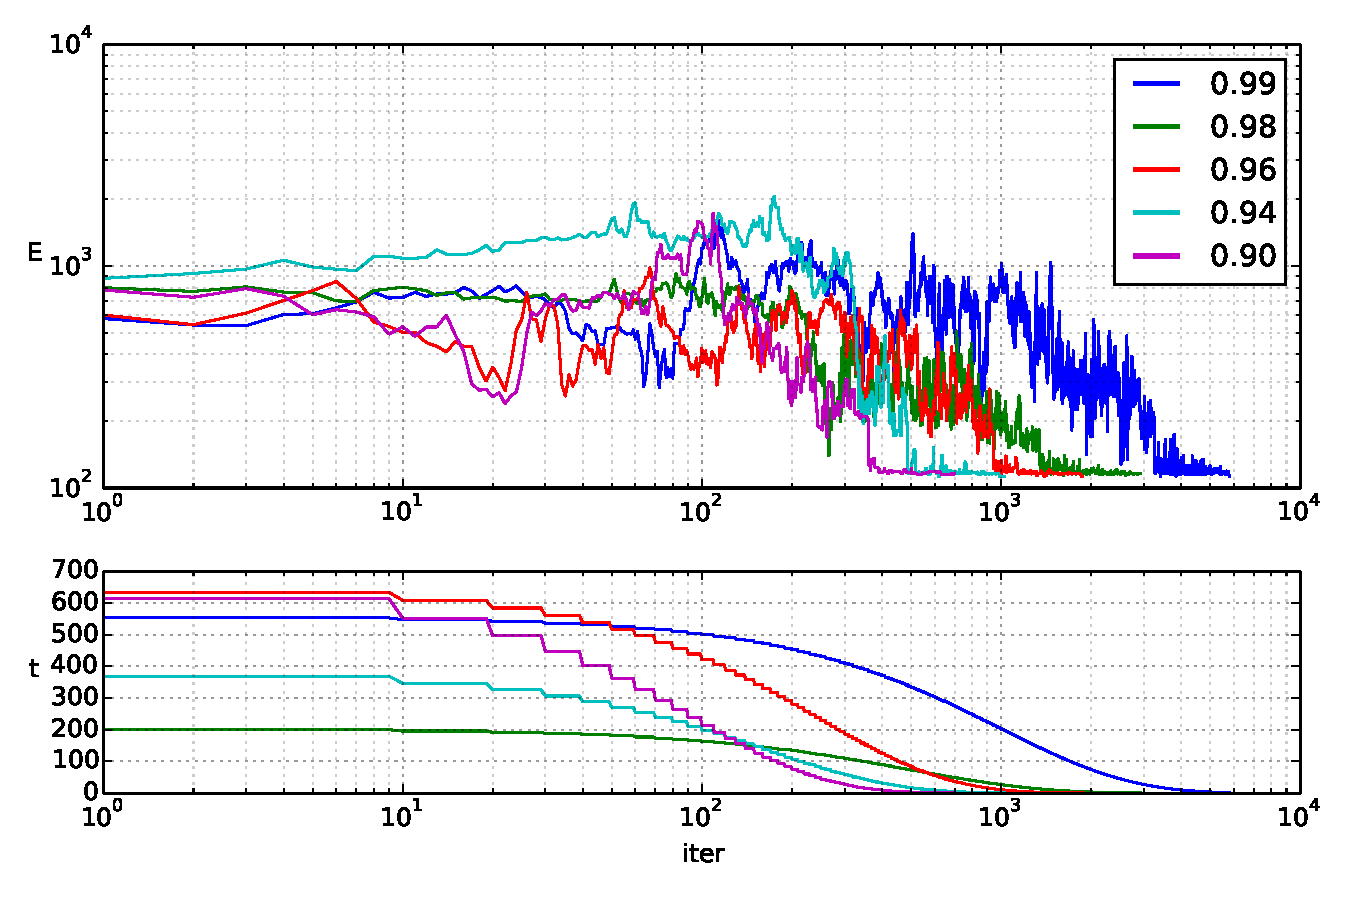
\includegraphics[width=1\linewidth]{figures/set2_walkers_temp.pdf}
    \caption{
        Kuvien \ref{fig:set2_datasets_res_99} -- \ref{fig:set2_datasets_res_90} kulkijoiden energioiden ja lämpötilojen kehitys.
        Stokastisen alkuarvon asetuksen takia alkulämpötilassa on huomattavaa vaihtelua ($t_0 \approx 200 \dots 700$).
        \label{fig:set2_walkers_temp}
    }
\end{figure}

\begin{figure}[p]
    \centering
    \makebox[\textwidth][c]{
        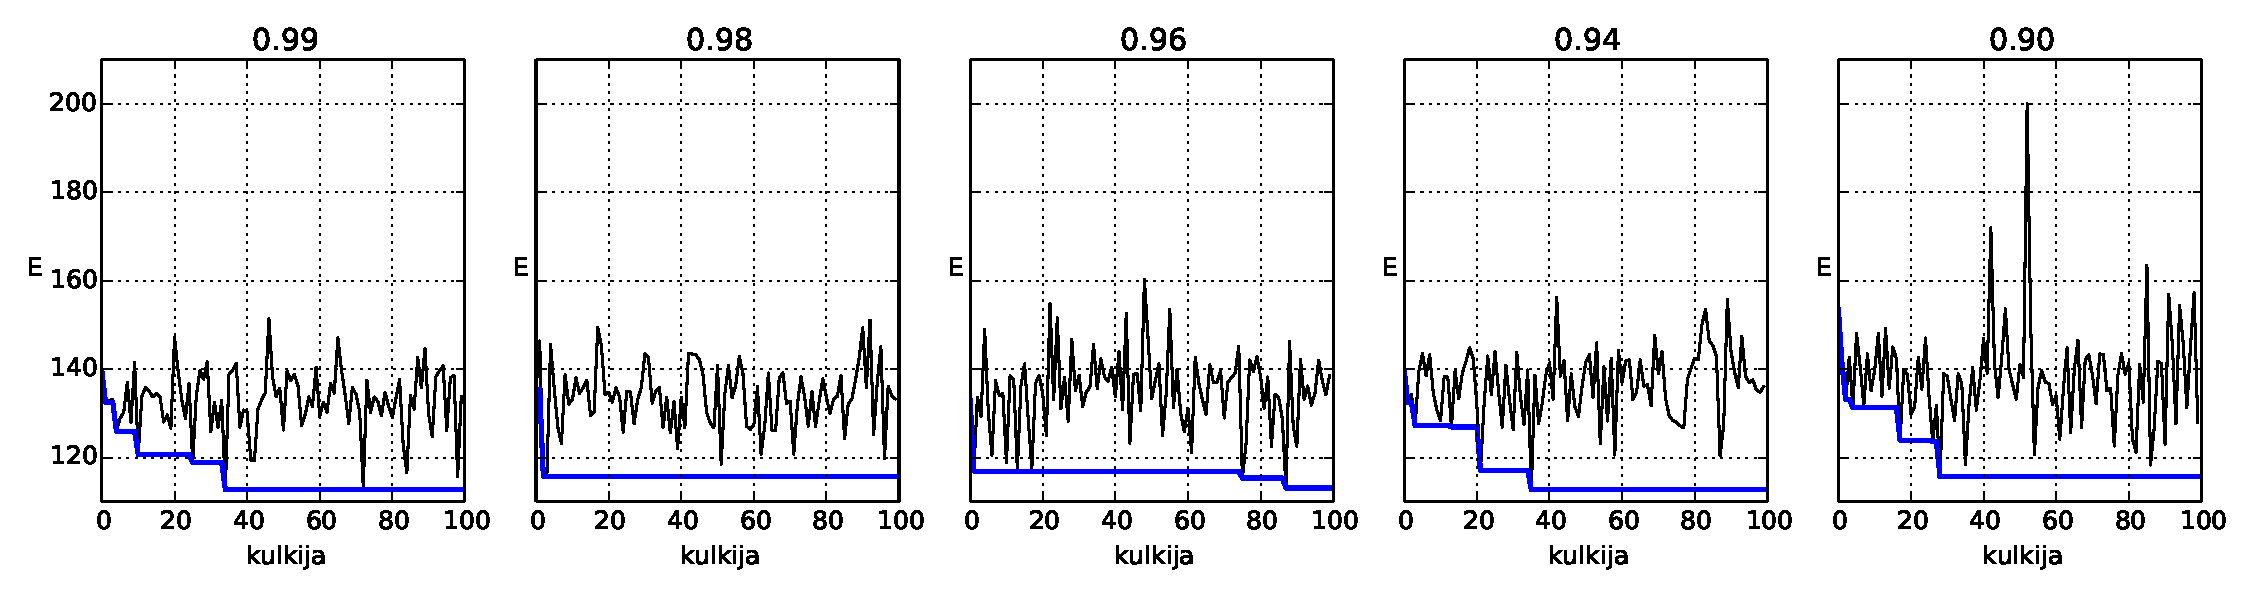
\includegraphics[width=1.4\linewidth]{figures/set2_best_final_e_walkers.pdf}
    }
    \caption{Kuvien \ref{fig:set2_datasets_res_99} -- \ref{fig:set2_datasets_res_90} vastaavien kokoelmien parhaan energian kehitys kokoelman koon funktiona.
        %Todo. Vastaava rivi histogrammeista?
        \label{fig:set2_best_final_e_walkers}
    }
\end{figure}

\FloatBarrier

\begin{table}[htpb]
    \centering
    \caption{Testiaineiston kuvat e,f. Kuvien~\ref{fig:set3_datasets_res_099} ja \ref{fig:set3_datasets_res_090} energiafunktion suhteen parhaiden ratkaisujen lopulliset energiat, virheet ja kulkijoiden pituus.
        \label{tab:3_res_errors}
    }
    \begin{tabular}{l c c c c c}
        $\alpha$ & Aineisto & Markov-ketjuja & Energia & $m_\text{sov}$ & $m_\text{symm}$ \\[2pt]
        \hline\noalign{\smallskip}
        0.99 & e & 636 & 126.820768777 & 41.7710820974 & 26 \\
             & f & 483 & 131.350277715 & 21.2525820166 & 58 \\[1pt]
        \hline\noalign{\smallskip}
        0.94 & e & 89  & 126.912392409 & 29.5102365738 & 36 \\
             & f & 102 & 134.677587474 & 27.8990164056 & 70 \\[1pt]
        \hline\noalign{\smallskip}
        0.90 & e & 74  & 124.101054568 & 11.8660423496 & 30 \\
             & f & 65  & 139.955257356 & 14.0600416833 & 92
    \end{tabular}
\end{table}

\begin{figure}[htpb]
    \centering
    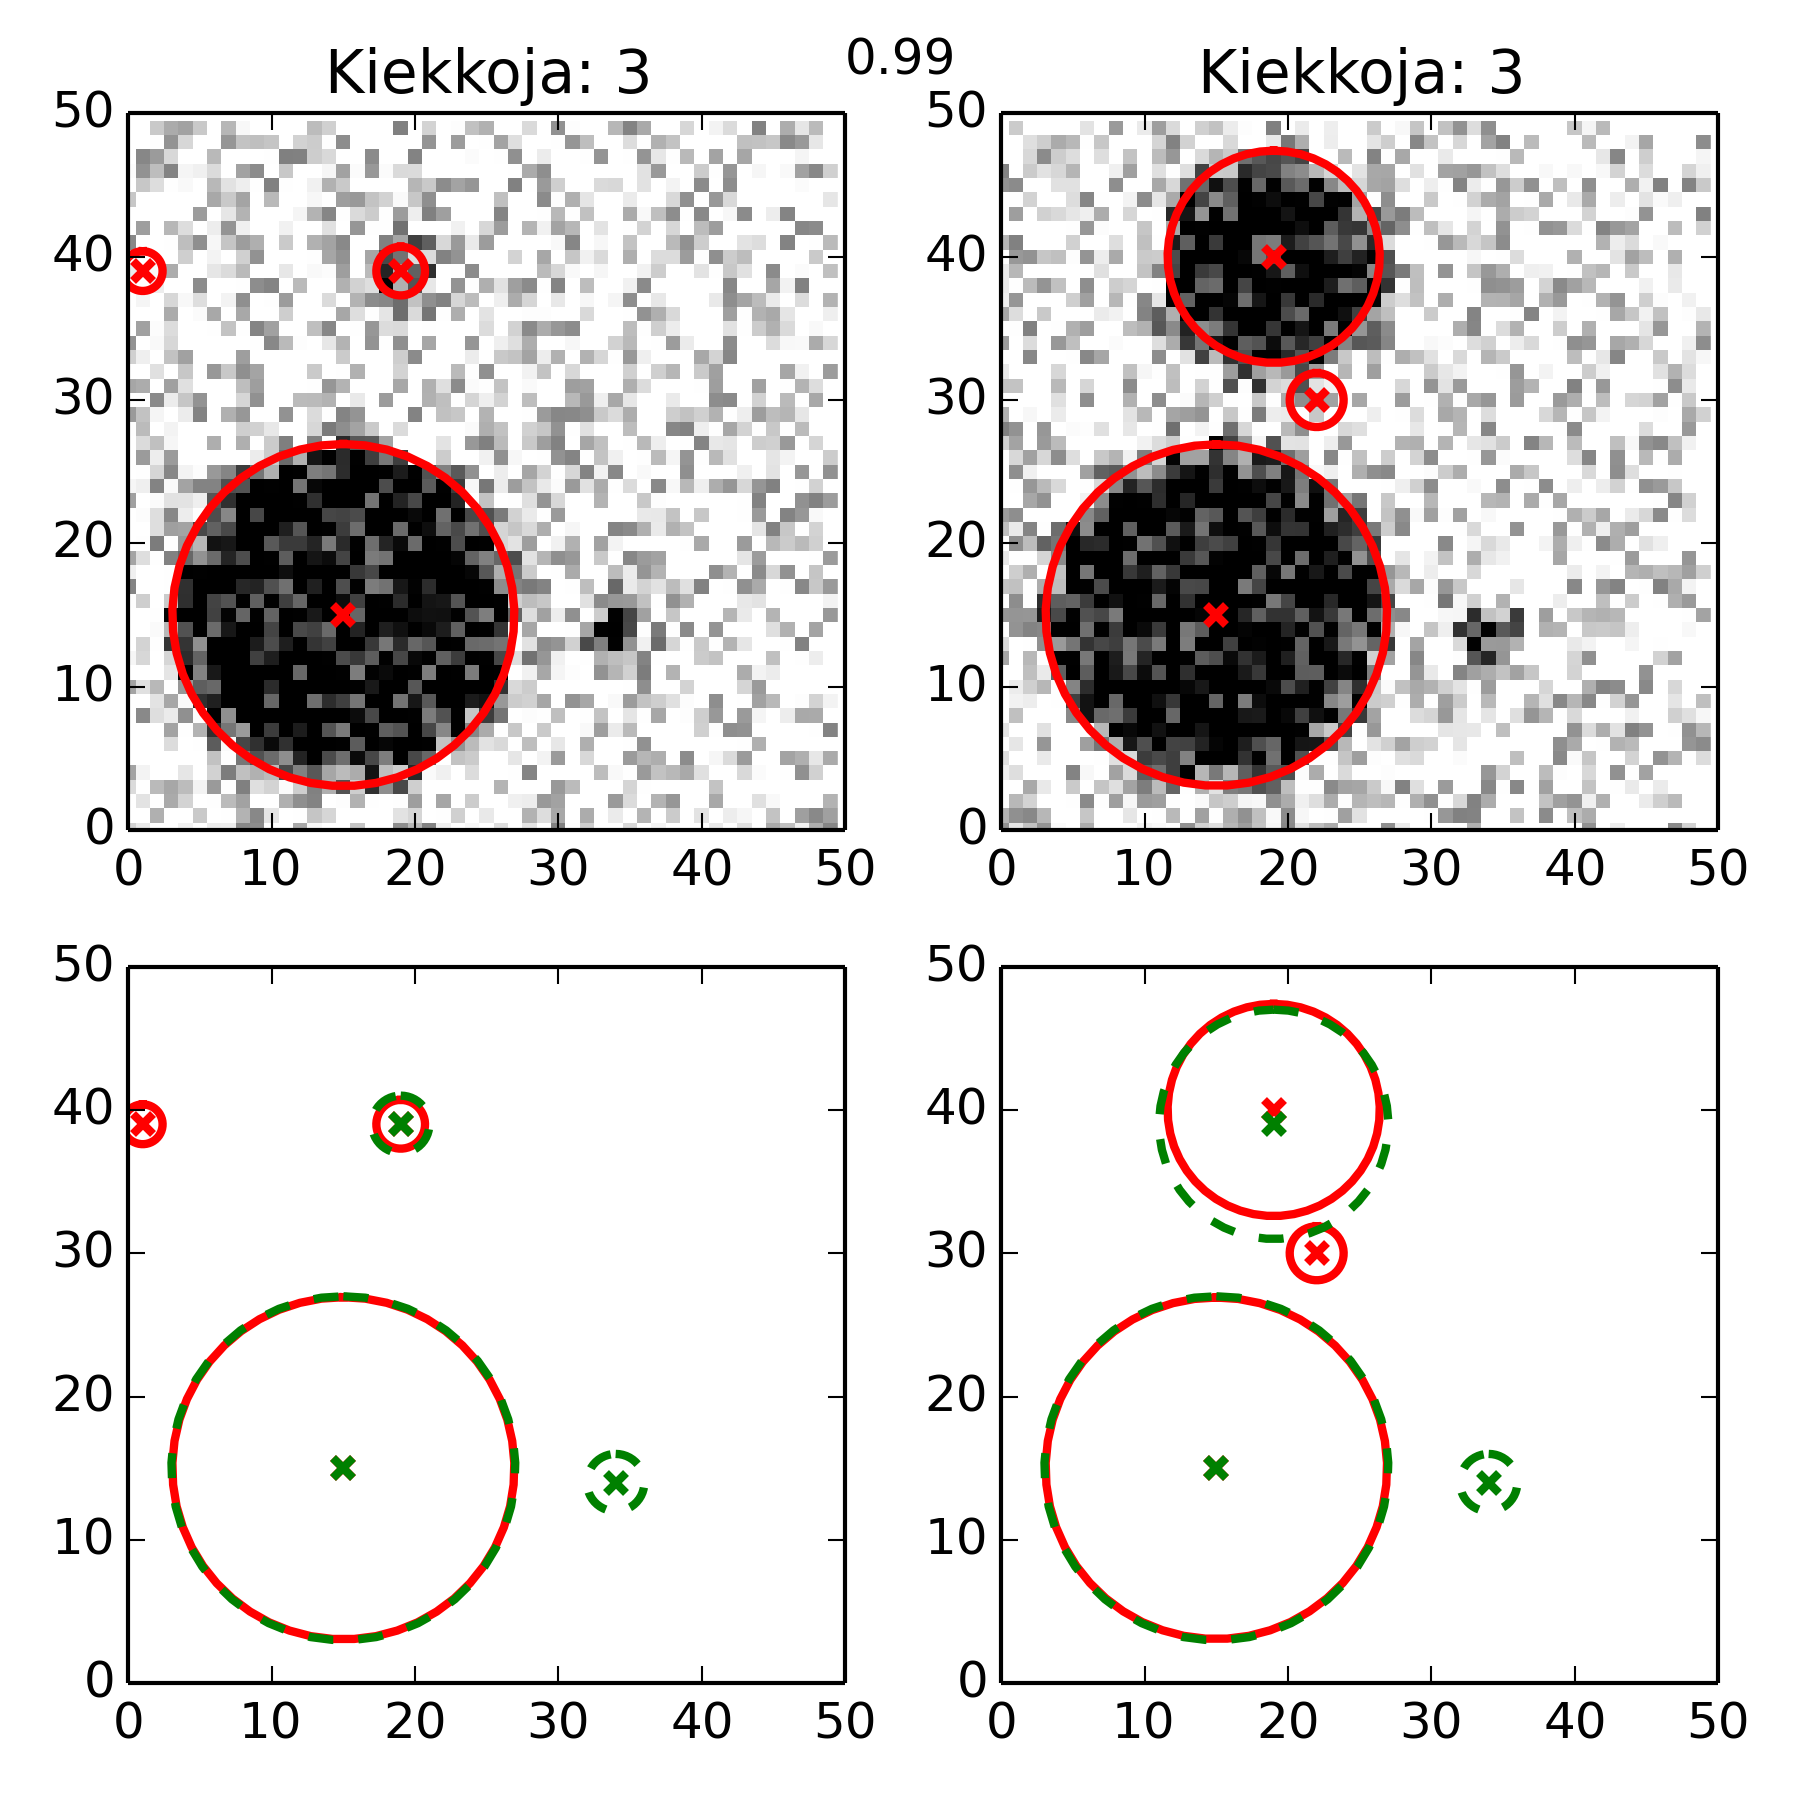
\includegraphics[width=0.7\linewidth]{figures/set3_datasets_res_099.png}
    \caption{
        Kuvat e, f: Parhaat ratkaisut (punaiset ympyrät) 100 kulkijan kokoelmasta jäähdytysskenaariolla $\alpha = 0.99$.
        \label{fig:set3_datasets_res_099}
    }
\end{figure}


\begin{figure}[htpb]
    \centering
    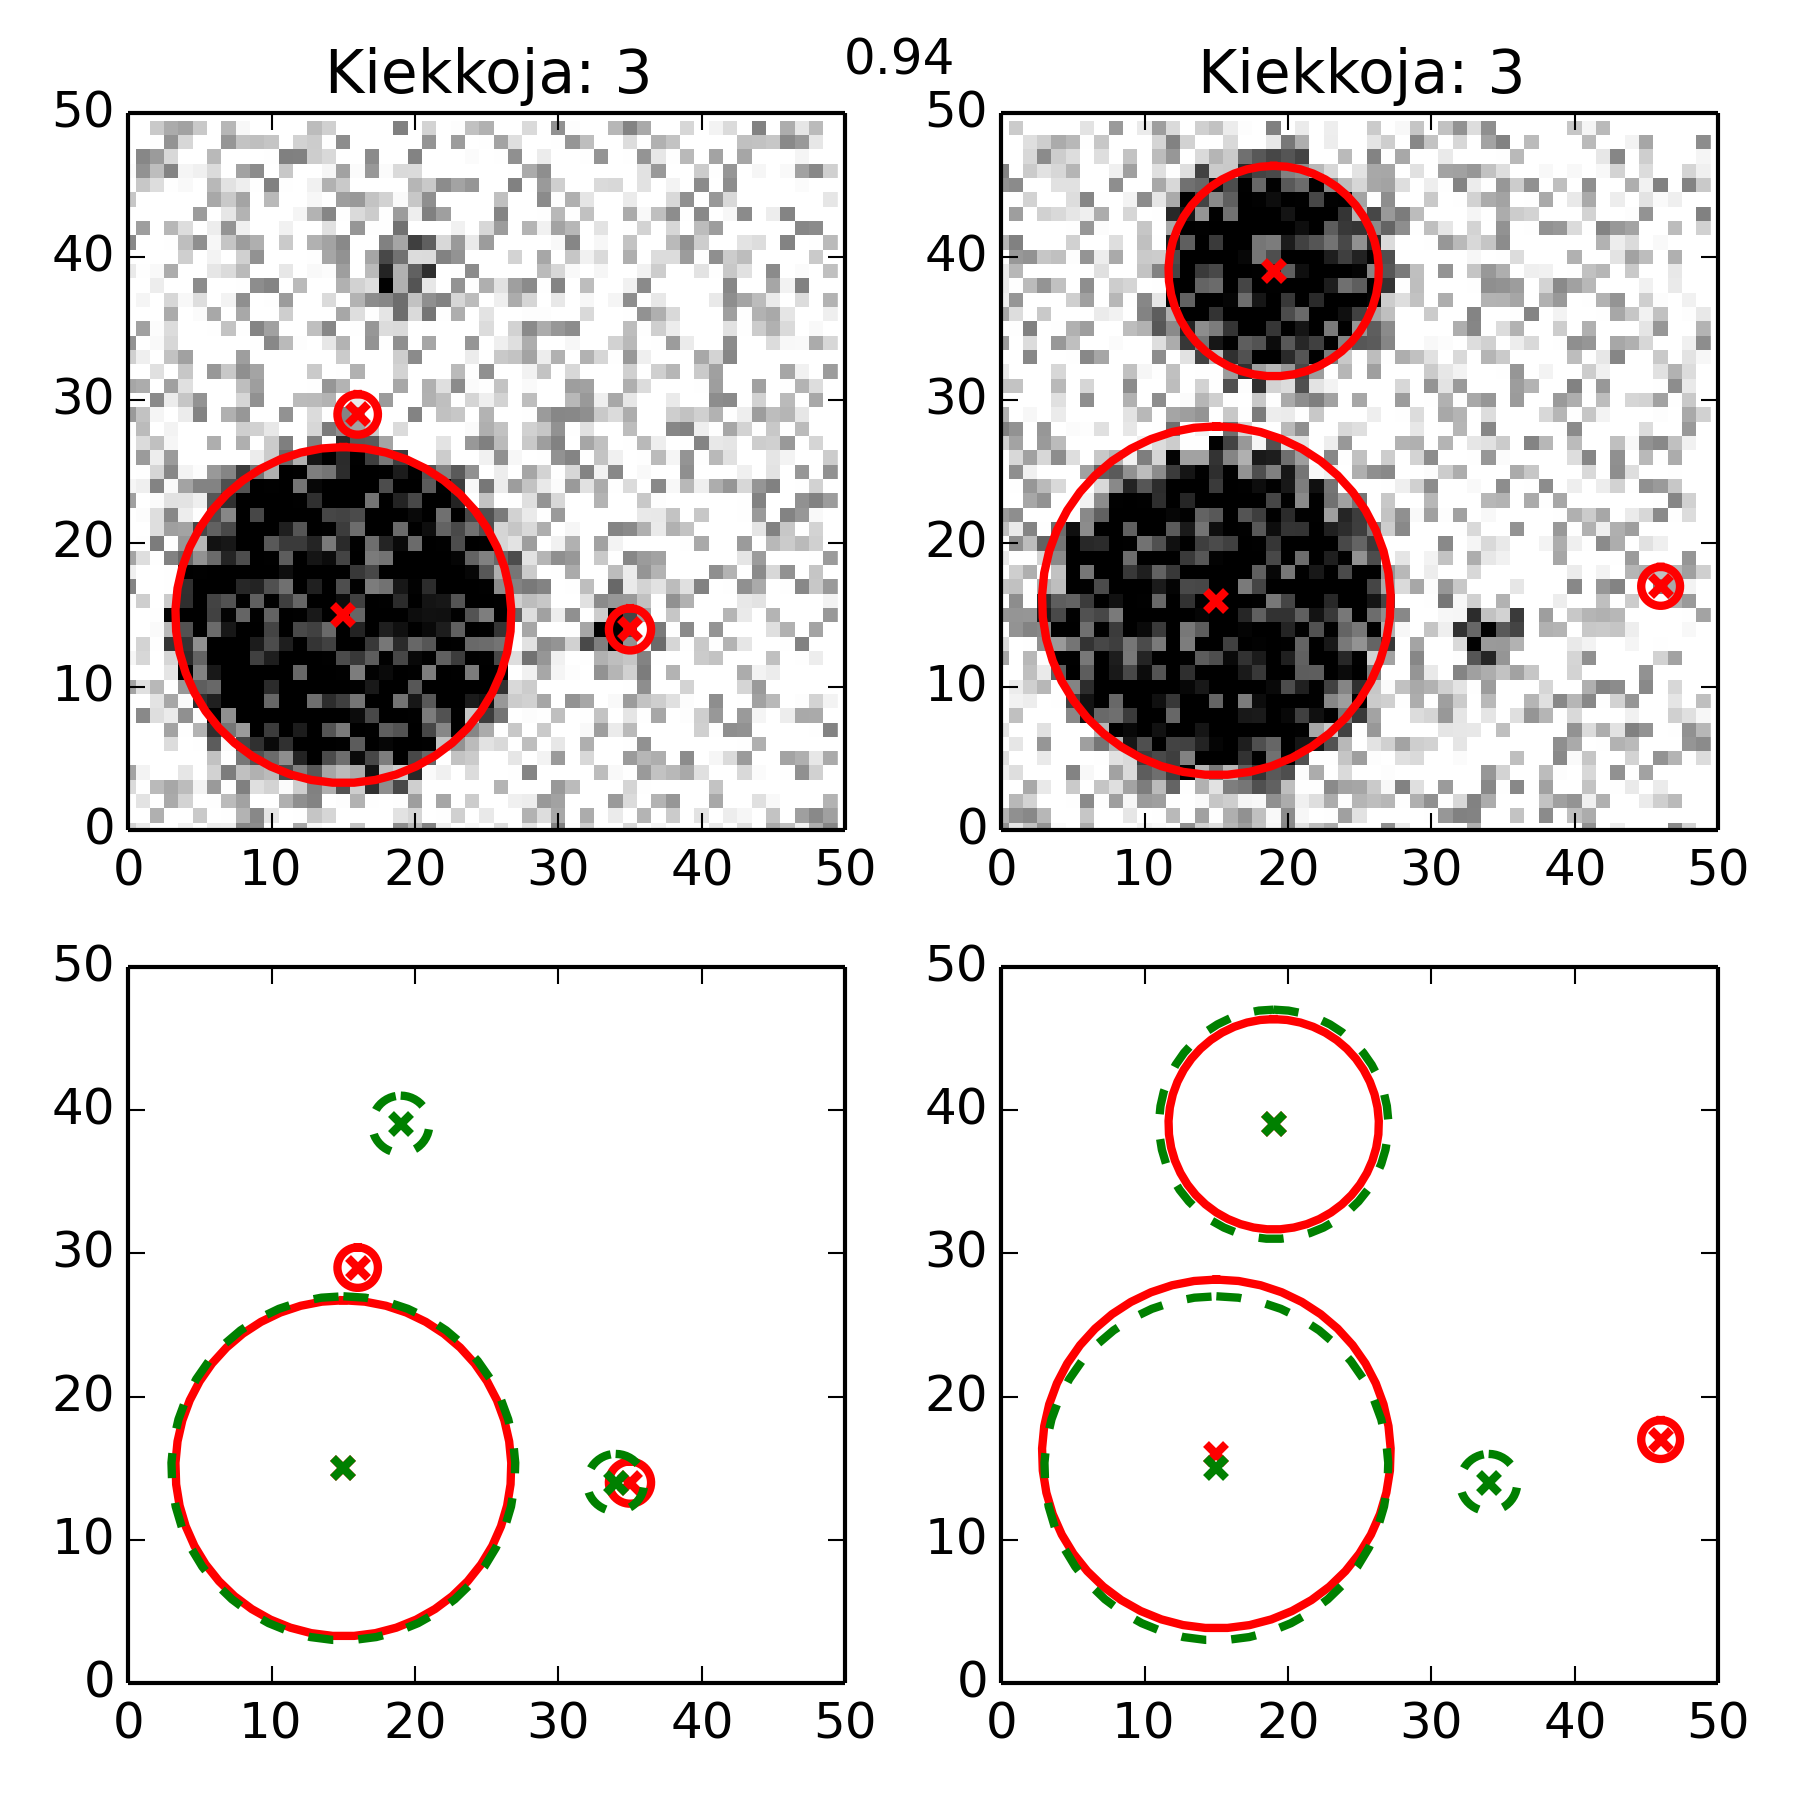
\includegraphics[width=0.7\linewidth]{figures/set3_datasets_res_094.png}
    \caption{
        Testikuvat e, f: Parhaat ratkaisut (punaiset ympyrät) 100 kulkijan kokoelmasta jäähdytysskenaariolla $\alpha = 0.94$.
        \label{fig:set3_datasets_res_094}
    }
\end{figure}


\begin{figure}[htpb]
    \centering
    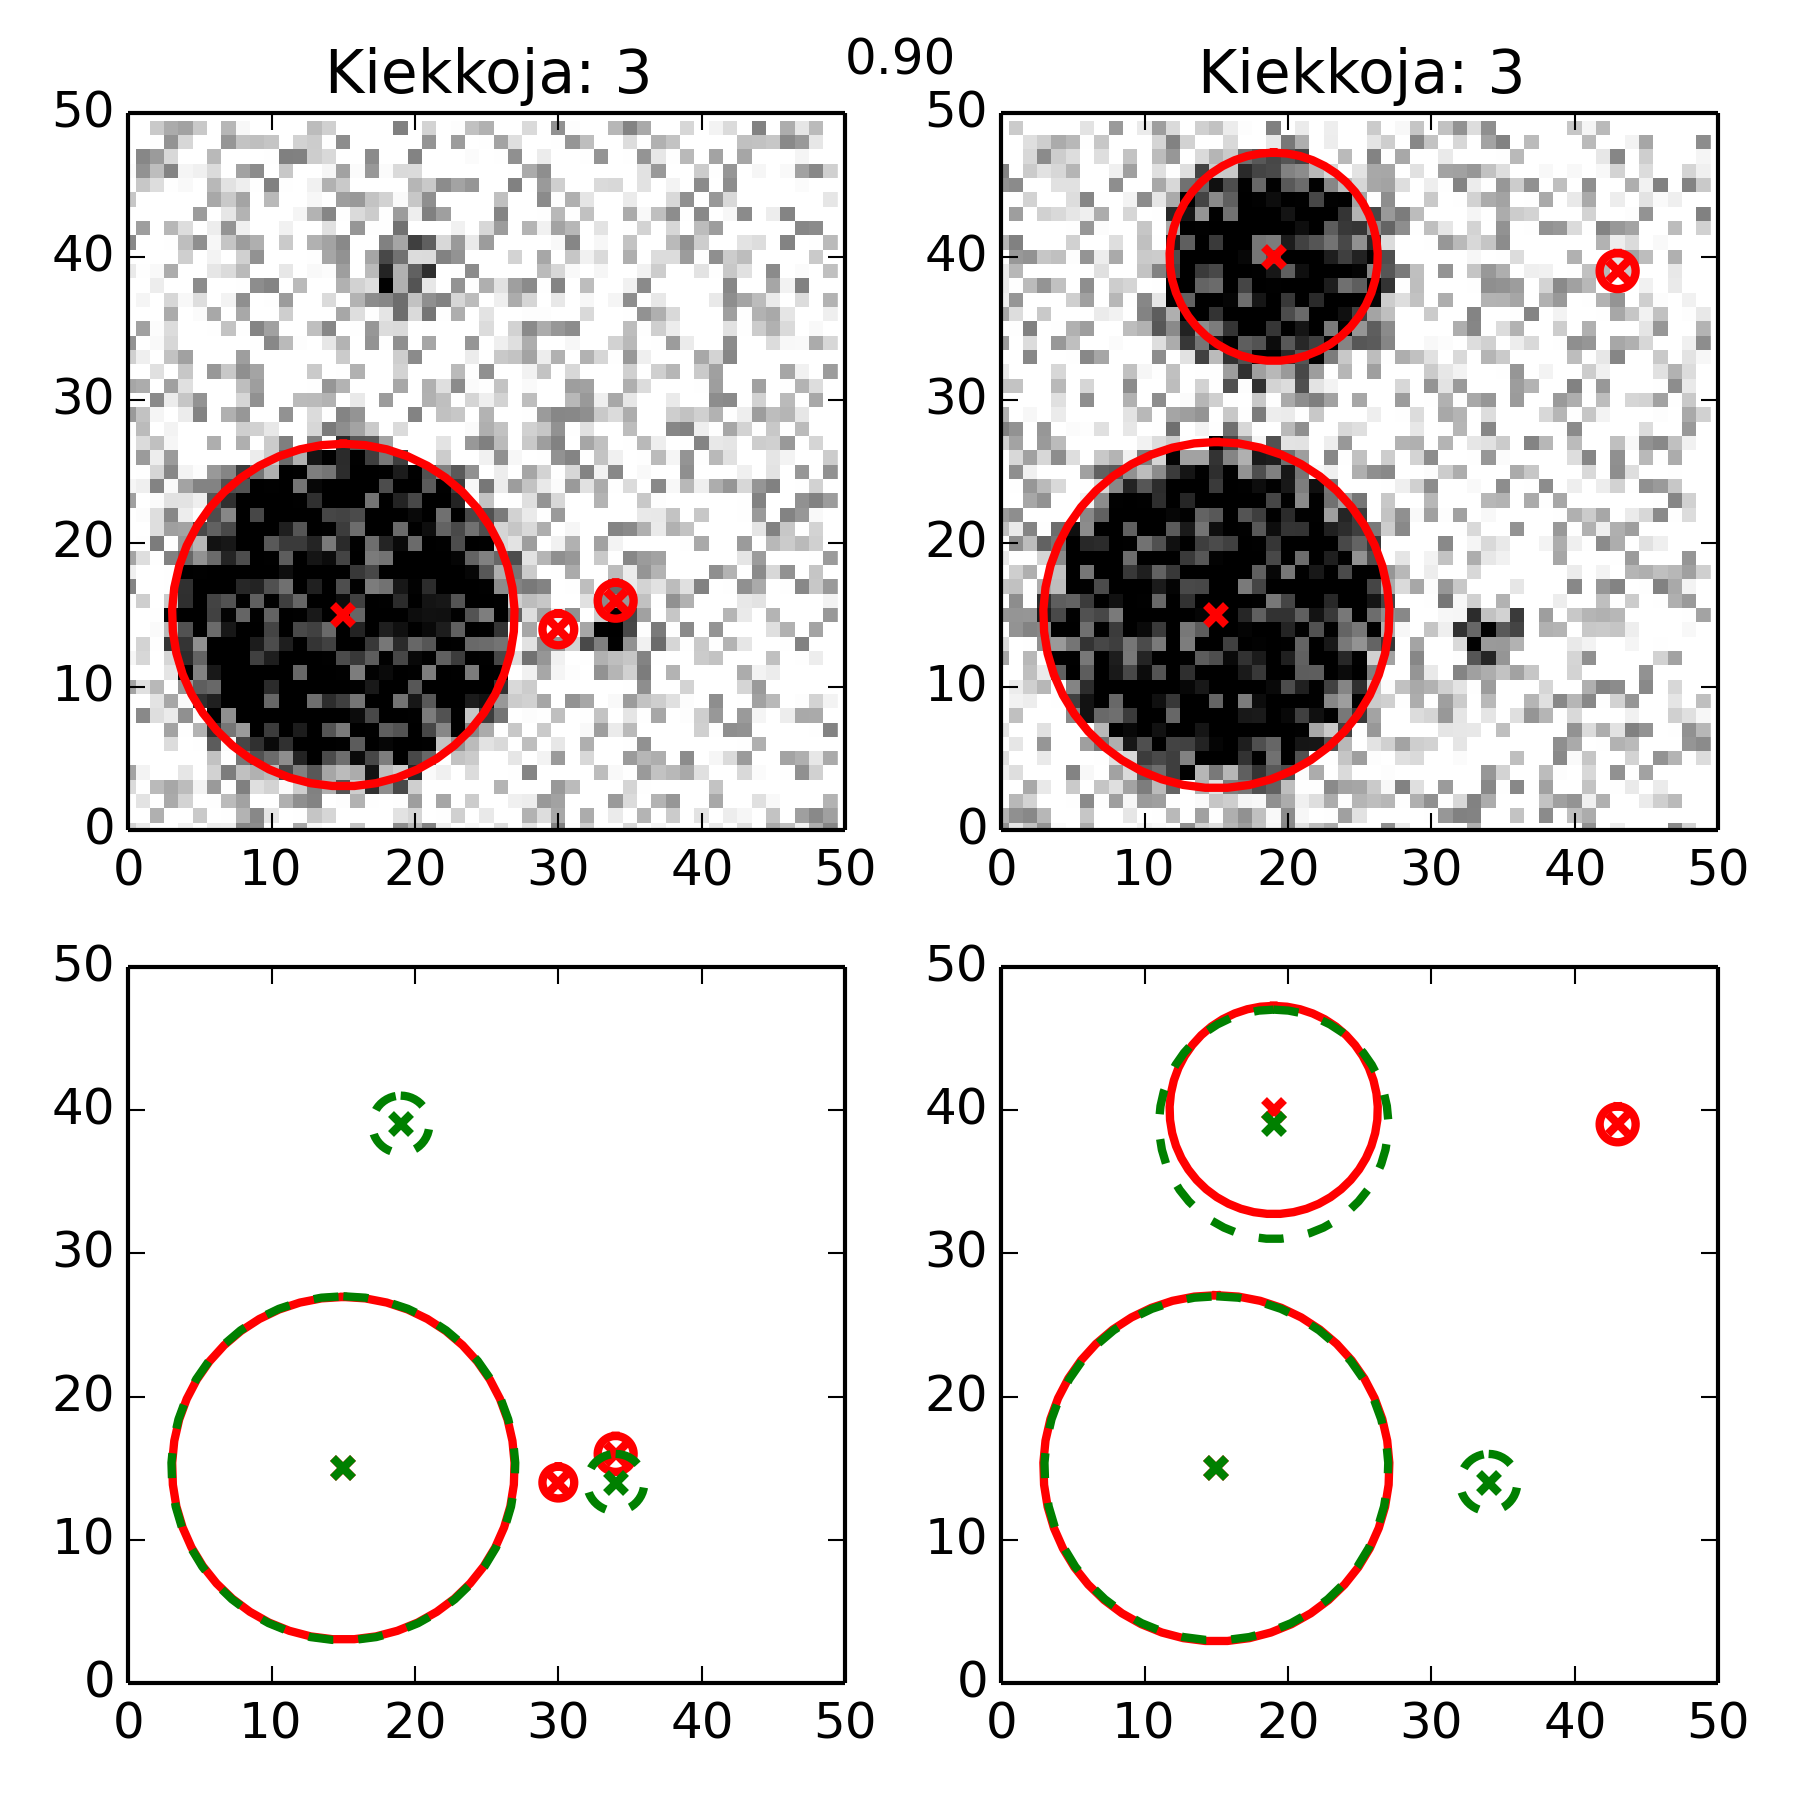
\includegraphics[width=0.7\linewidth]{figures/set3_datasets_res_090.png}
    \caption{
        Testikuvat e, f: Parhaat ratkaisut (punaiset ympyrät) 100 kulkijan kokoelmasta jäähdytysskenaariolla $\alpha = 0.90$.
        \label{fig:set3_datasets_res_090}
    }
\end{figure}


\begin{figure}[htpb]
    \centering
    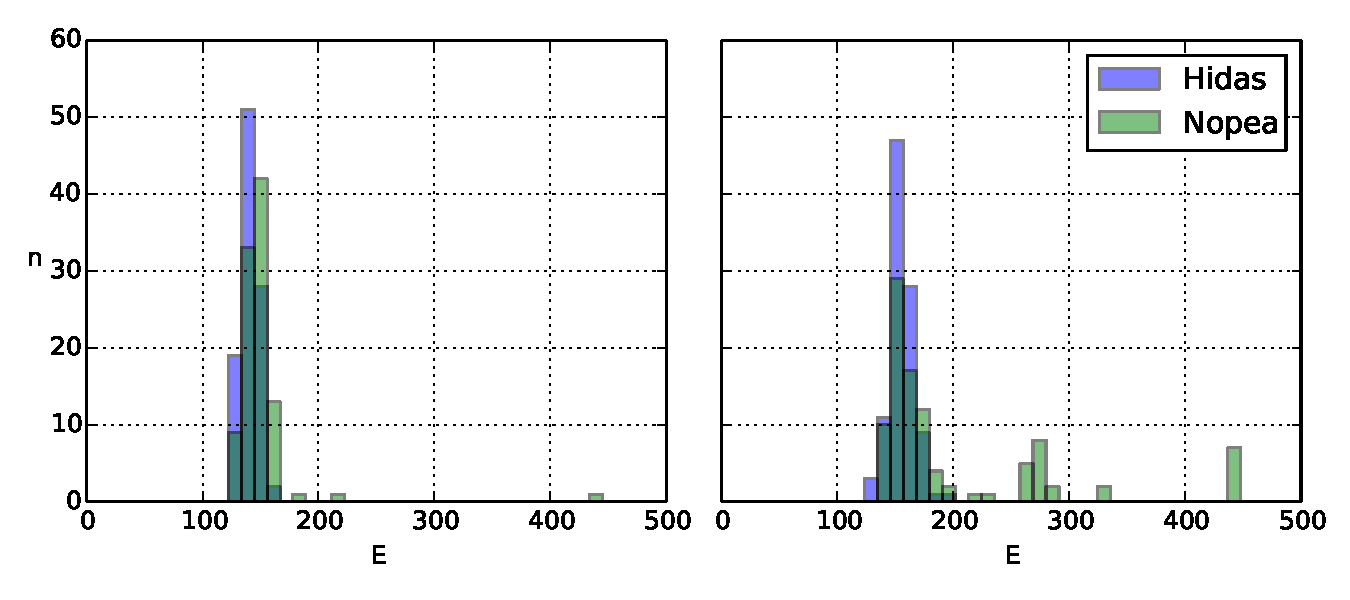
\includegraphics[width=1.0\linewidth]{figures/set3_histo_compare_2_099_090.pdf}
    \caption{Testikuvien e ja f kulkijakokoelmien loppuenergiajakaumien histogrammit jäähdytysskenaarioilla $\alpha = 0.99$ (hidas) ja $\alpha = 0.90$ (nopea)
        \label{fig:set3_histo_compare_2_099_090}
    }
\end{figure}

%Kaikkien kokoelmien lopulliset energiajakaumat. (Loppuenergioiden jakauma)
%
%Kullekin kokoelmalle kaikkein paras energia kulkijoiden määrän funktiona.
%
%Kaikkein parasta energiaa vastaavat ratkaisut.
%
%Niiden virheet.
%
%Tyypillisen / keskimääräisen kävelijän energia ja sitä vastaava ratkaisu.
%
%Graafi kävelijöistä isossa ja pienessä ongelmassa.



    \chapter{Pohdinta ja johtopäätökset}
\label{cha:pohdinta}

\section{Tulosten analyysi}
\label{sec:tulosten_analyysi}

\subsection{Energiafunktio}
\label{sub:pohdinta_energiafunktio}

Luvussa~\ref{sec:algoritmin_tulokset} esitettyjen tulosten perusteella voidaan todeta että algoritmi toimii yleensä kelvollisesti.
Silmämääräisesti energiafunktioltaan parhaat ratkaisukiekot ovat usein varsin lähellä oikeaa.
Energiafunktion teoreettista globaalia minimiä voidaan arvioida laskemalla energiafunktion $E_\text{naiivi}$ odotusarvo $\E$ $50x50$-kokoiselle kuvalle, jossa teoreettisen ihanteellisten ratkaisuympyröiden $P \ast A_W$ peittäessä datan ympyrät on jäljellä pelkkää mallin mukaista satunnaiskohinaa.
Odotusarvoksi saadaan
\begin{align}
    \E \Big[ E_\text{naiivi}([E]_{>0}) \Big] &= \E \Big[ \sum_{i,j} [E(i,j)]_{>0}^2 \Big],\\
    \intertext{
        missä kukin matriisin $[E]_{>0}$ alkio $[E(i,j)]_{>0}$ on yhtälön~\eqref{eq:leikkaus} mukainen satunnaismuuttuja, joka saadaan 'leikkaamalla' $U(-0.5, 0.5)$-jakautunut muuttuja $E(i,j)$ välille $[0,1]$,
        jolloin kun satunnaismuuttujan $E(i,j)$ tiheysfunktiota merkitään $p_{E(i,j)}(x)$
    }
    \label{eq:teorglob1}
    &= \sum_{i,j} \E \Big[ [E(i,j)]_{>0}^2 \Big] \\
    \label{eq:teorglob2}
    &= \sum_{i,j} \left( \int_0^{0.5} x^2 p_{E(i,j)}(x) dx + \int_{-0.5}^0 0 \cdot p_{E(i,j)}(x) dx \right)\\
    &= \sum_{i,j} \Big[\frac{x^3}{3}\Big]^{0.5}_{0} = \sum_{i,j} \frac{1}{3 \cdot 8} = \sum_{i,j} \frac{1}{24}\\
    &= \frac{50\cdot50}{24} \approx 104.17,
\end{align}
mikä on hyvin lähellä muutamia myös silmämääräisesti erikoisen hyvin onnistuneiden ratkaisujen lopullisia energiatasoja, esimerkkinä kuvan~\ref{fig:set2_datasets_res_99} ratkaisu, jonka loppunenergia $\approx 112.71$ (taulukossa~\ref{tab:2_res_errors}).
Toisaalta pitää myös huomioida, että simuloidun datan ja mallin erojen ynnä muiden virheiden vuoksi on epärealistista odottaa tällaista ideaalista ratkaisua, jossa energiafunktiolla arvioitaisiin kuvaa josta kiekot olisi poistettu täydellisesti ja jäljellä olisi vain kohinaa.

Yllä vaihe~\eqref{eq:teorglob1} seuraa odotusarvon lineaarisuudesta ja \eqref{eq:teorglob2} yleisestä kaavasta muunnetun (myös sekatyyppisen) satunnaismuuttujan odotusarvolle,
\begin{equation*}
    \E [g(X)] = \int_{-\infty}^{\infty} g(x) p_X(x) dx,
\end{equation*}
joiden tarkemmat perustelut löytyvät esimerkiksi luentomonisteessa~\cite{koistinen2013}.

Toisaalta kuten jaksoissa~\ref{sub:energiamaasto} ja \ref{sub:paranneltu_monen_kiekon_energiafunktio} oletettiin, paranneltu energiafunktio $E_\text{par}$ ei ole täydellinen:
ihmissilmään suunnilleen oikeissa paikoissa sijaitsevat mutta hieman epätarkasti $A_\text{data}$:n peittävät ratkaisukiekot, kuten kuvassa~\ref{fig:A_datasets_res_fast} viiden kiekon testidatan c ratkaisu ($\alpha = 0.90$, loppuenergia $\approx 159.5$), on parempi ratkaisu kuin esimerkiksi saman datan toinen ratkaisu (kuvassa~\ref{fig:A_datasets_res_fast}, $\alpha = 0.99$, energia $\approx 149.5$)
jossa suuret kiekot ovat sijoittuneet tarkemmin kuin $\alpha = 0.90$ -skenaariossa mutta yksi pieni kiekko täysin väärässä paikassa.
Energiafunktio ja $m_\text{symm}$ ovat arvoltaan kuitenkin kyseisellä silminnähden huonommalla ratkaisulla parempia, toisin kuin intuitiota paremmin vastaava mitta $m_\text{sov}$.
Suurten kiekkojen pienetkin virheet näkyvät suuren pinta-alansa vuoksi energiafunktiossa ja virhemitasssa $m_\text{symm}$ herkästi.
Näin ollen ylipäätään pienet kiekot olivat algoritmille vaikeita, kuvat~\ref{fig:set3_datasets_res_099} -- \ref{fig:set3_datasets_res_090}.

\subsection{Jäähdytysstrategiat}
\label{sub:pohdinta_jaahdytysstrategiat}

Samoin kuten jäähdytysmenetelmän kirjallisuus antaa olettaa, hitaat jäähdytysskenaariot saavuttavat jossain määrin parempia tuloksia kuin hitaat.
Vaikka sadan kulkijan joukosta valikoidut kaikkein parhaat ratkaisut saavat kaikki melko hyviä ja varsin samanlaisia tuloksia kaikilla $\alpha$ (kuvat~\ref{fig:set2_datasets_res_99} -- \ref{fig:set2_datasets_res_90}, \ref{fig:set3_datasets_res_099} -- \ref{fig:set3_datasets_res_090}), hitaan ja hieman nopeamman jäähdytyksen ero näkyy kaikkien kulkijoiden loppuenergioiden histogrammissa~\ref{fig:set3_histo_compare_2_099_090}:
Nopeilla skenaarioilla histogrammin massa on oikeammalla.

Lisäksi havaitaan että useiden kiekkojen ongelmissa jakauma ei ole aina unimodaalinen,
vaan erityisesti nopeilla strategioilla huomattavan moni kulkija voi 'jäähtyä' epäedulliseen konfiguraatioon jossa vain osa kiekoista löydetään.
(Havainnollistava kuva~\ref{fig:A_modalbin_cc_fast_1}, vastaavia piikkejä myös \ref{fig:set3_histo_compare_2_099_090}.)

Toisaalta kuitenkin vastapainona nopealle jäähdytysstrategialla kulkijakokoelman kokoa kasvattamalla todennäköisyyttä että nopeakin jäähdytys löytää hyvän tuloksen (kuva~\ref{fig:set2_best_final_e_walkers}).
Yleisesti jäähdytysmenetelmän kaltaisten algoritmien tehokkaassa soveltamisessa numeerisesti raskaissa ongelmissa usein onkin hyödyllistä yrittää löytää optimaalinen suhde jäähdytysskenaarion pituuden ja kulkijakokoelman koon välillä, ja etenkin sen dynaaminen arvioiminen ongelmanratkaisun aikana \cite{salamonetal}.

\subsection{Ulottuvuuskirous}
\label{sub:ulottuvuuskirous}

Kiekkojen lukumäärän kasvaessa yhdellä ongelman optimoitavien parametrien avaruuden ulottuvuus kasvaa kolmella.
Tunnetusti optimointiongelmissa tämä avaruuden koon kasvu vaikeuttaa optimointiongelmia, ja tästä syystä kiekkojen määrä oletettiin tunnetuksi vakioksi.
Näin ollen vielä tutkielman pienillä kiekkomäärillä $k = 1, \dots, 5$ ulottuvuuksien kasvu ei näyttänyt olevan jäähdytysalgoritmille suuri ongelma.

\section{Yhteenveto ja pohdinta}
\label{sec:johtopaatokset}

\subsection{Algoritmi}
\label{sub:jp_algoritmi}

Jäähdytysalgoritmi löysi esitettyyn kuvaongelmaan hyvän ratkaisun melko luotettavasti,
joten tässä mielessä metodia voi pitää toimivana.
SA on vakiintunut menetelmä, josta on laajalti monenlaisia sovelluksia.
Tässä tutkielmassa sovellettiin perinteistä jäähdytysalgoritmin muotoilua hyvin yksinkertaisella jäähdytysskenaariolla.
Myös toiminnan analysointiin ja parantelemiseen kuhunkin ongelmaan sopivaksi kirjallisuus esittelee runsaasti termodynamiisesta analogiasta inspiroituneita työkaluja,
joiden käsittely jää tämän tutkielman ulkopuolelle.
(Esimerkiksi tilastollisen mekaniikan käsitteiden, kuten jäähdytettevän ongelman 'ominaislämmön' tai 'entropian', hyödyntäminen ongelman rakenteen tutkimisessa, tai jäähdytysskenaarion tai siirtojen optimoinnissa , \cite[ks.][]{salamonetal}.
Nykyisenlaajuisessa tarkastelussa soveltamalla algoritmia erilaisiin ympyräkuviin erilaisilla jäähdytysskenaarioilla havaittiin SA:lle tyypillistä käytöstä.

\subsection{Konenäkötehtävä}
\label{sub:jp_konenako}

Kuten luvussa~\customref{cha:johdanto} todettiin, oletettu kuvantunnistusongelma on melko yksinkertainen:

Esimerkiksi kiekkojen määrän olettaminen tunnetuksi on rajoittava yksinkertaistus.
SA-algoritmia voisi laajentaa kasvattamalla parametriavaruuden kokoa oletettuun ympyröiden maksimimäärään,
mutta vastavuoroisesti ulottuvuuksien määrä kasvattaisi ongelman kokoa.
Eräs mielenkiintoinen vaihtoehto voisi olla soveltaa jotain perinteistä erillisten yhtenäisten komponenttien laskemiseen (\emph{connected-component labeling}) tunnettua algoritmia \cite{cormenetal09} objektien lukumäärän selvittämiseen,
ja sitten soveltaa tässä esitettyä SA-algoritmia.
(Kappaleiden laskemista kuvassa voidaan myös lähestyä yleisenä ongelmana koneoppimisen menetelmin, kuten esimerkiksi \cite{lempitskyzissermanNIPS10}.)

Toisaalta myös erilliset ympyrät ovat myös melko rajoittunut malli monimutkaisempien muotojen mallintamiseen.
Tällaisten vaikeuksien vuoksi konenäön alalla muotojen mallintamisessa  tässä tutkielmassa käytetyn kaltaisten geometristen mallia sijasta suositumpia ovat erilaisiin merkitseviin pisteisiin perustuvat mallit (esimerkiksi \emph{active contour model, snakes} \cite{prince2012}).

Yhteenvetona, yleisesti reaalimaailman dekonvoluutiosovelluksia ajatellen tässä tutkielmassa käsitelty ongelma on rajoittunut.
Usein tutkittavan kuvan rakenteesta ei voida tehdä samanlaisia oletuksia kuten tässä tutkielmassa, ja joudutaan käyttämään paljon yleisempiä malleja.
Mutta ''oikeiden'' konenäön ongelmien ratkaisemiseen käytetään yleisellä tasolla hyvin samankaltaisia metodeja:
Sumennosta kuitenkin mallinnetaan konvoluutio-operaationa,
ja ratkaisun lähtökohtana on usein muodostetaan jokin sopiva energiafunktio, jota optimoidaan.


    % kirjallisuusviitteet
    \printbibliography[heading=bibintoc]
\end{document}
